\chapter{Hardwarová část}

Na obrázku \ref{fig:otopna-soustava-a-elektronika-rez-domu} je nákres otopné soustavy včetně jednotlivých zařízení pro ovládání této soustavy. V~textu dále popíši jednotlivá vybraná či navržená zařízení z~nákresu (pro přehlednost jsou jednotlivé části uvozeny výřezem obrázku dané části z celkového nákresu), které jsem realizoval nebo zakoupil hotové, případně je upravil. Dále uvedu popis pro zrealizované nástěnné snímače prostorové teploty.

\newpage

\begin{figure}[H]
    \centering
    \def\svgwidth{\columnwidth}
    \input{images/svg/otopna-soustava/otopna-soustava-a-elektronika-rez-domu1.pdf_tex}
    \caption{Otopná soustava v domě včetně elektroniky pro řízení.}
    \label{fig:otopna-soustava-a-elektronika-rez-domu}
\end{figure}


\section{Centrální jednotka Raspberry Pi}


\begin{figure}[H]
    \centering
    \def\svgwidth{0.3\columnwidth}
    \input{images/svg/otopna-soustava/vyrez-centralni-jednotka.pdf_tex}
    \caption[Výřez pro centrální jednotku.]{Výřez z obrázku \ref{fig:otopna-soustava-a-elektronika-rez-domu} – centrální jednotka.}
    \label{fig:vyrez-centralni-jednotka}
\end{figure}

Na obrázku \ref{fig:vyrez-centralni-jednotka} je výřez části z celkového nákresu (obrázek \ref{fig:otopna-soustava-a-elektronika-rez-domu}) pro centrální jednotku . Pro centrální řídicí jednotku byl vybrán jednodeskový počítač Raspberry Pi model 4 \cite{raspberry-pi}. Důvodem pro vybraní byla přímá podpora HA, velká uživatelská základna, která toto zařízení používá (nejen s HA, ale i s jiným softwarem), nízká cena a relativně vysoký výkon. Přehled specifikace zařízení je na stránkách výrobce \cite{raspberry-pi}. Samozřejmě může vzniknout úvaha nad odolností tohoto zařízení např. vůči vnějšímu rušení, samotného rušení zařízení apod. Co se týče nasazení takového zařízení, většinou výrobci uvádějí že se jedná o~vývojové zařízení, které není určeno do koncového zařízení nebo případně splňují  základní certifikace ochrany. Průmyslovou certifikaci nesplňují nebo se na trhu nacházejí zařízení, které se průmyslovou aplikací chlubí (zde je nutné důkladně pročíst všechnu technickou dokumentaci), pak dále skutečně stojí za zvážení o jakou certifikaci se jedná, v jaké části průmyslu lze toto zařízení nasadit, ale i tak to může být dost velký risk. Ve většině případů je však nutné provést hardwarovou úpravu pro vysokou odolnost proti rušení, robustnost běžícího real time systému, RTC, typ paměti pro ukládání dat (typ média), životnost, technická podpora a mnohé další. V~domácích podmínkách nejsou nutné všechny požadavky jako v průmyslu, nicméně je nutné minimálně hledět na \acrshort{esd} (\textit{\acrlong{esd}}) ochranu připojených periferií především u sběrnic, které jsou na delší vzdálenosti a~způsob ukládání dat z pohledu životnosti paměťového média. Pro ESD ochranu jak samotného Raspberry Pi, tak i~koncových zařízení je nutné zapojit mezi kabely sběrnice a zařízení ESD ochrany (takové ochrany jsou navrženy a~popsány níže). SD kartu pro ukládání a běh samotného systému je vhodné změnit za médium s~vetší životností, lze využít například domácí NAS a data ukládat do databáze, SD kartu používat pouze pro systém či USB flash disk. Případně zajistit postup s předpřipravenou zálohou pro obnovu nefunkčního systému apod. 

\section{Teplotní senzory}

\begin{figure}[H]
\centering
\begin{subfigure}{.5\textwidth}
    \centering
    \input{images/svg/otopna-soustava/vyrez-teplotni-senzory-krb.pdf_tex}
    \caption{Teplotní senzor na kouřovodu krbu.}
    \label{fig:vyrez-teplotni-senzory-krb}
\end{subfigure}%
\begin{subfigure}{.5\textwidth}
   	\centering
   	\input{images/svg/otopna-soustava/vyrez-teplotni-senzory-zasobnik-otopne-vody.pdf_tex}
     \caption{Teplotní senzory v zásobníku otopné vody.}
    \label{fig:vyrez-teplotni-senzory-zasobnik-otopne-vody}
\end{subfigure}%
\caption[Výřez pro umístění teplotních senzorů.]{Výřez z obrázku \ref{fig:otopna-soustava-a-elektronika-rez-domu} – umístění teplotních senzorů.}
\end{figure}

Na obrázku \ref{fig:vyrez-teplotni-senzory-krb} je výřez části z celkového nákresu (obrázek \ref{fig:otopna-soustava-a-elektronika-rez-domu}) pro umístění teplotních senzorů u kouřovodu krbu. Pro snímání teploty z kouřovodů u krbů slouží termočlánek typu K od výrobce Guenther. Teplotní rozsah je od -100 °C do 400 °C, takže je dostatečná teplotní rezerva. Průměr kovové ochranné trubičky je 4 mm s délkou 60 mm. Přívodní kabel je dlouhý 3 m se skelným opletením. Termočlánek je zobrazen na obrázku \ref{fig:termoclanek-72-21301041-k}.

\begin{figure}[H]
    \centering
    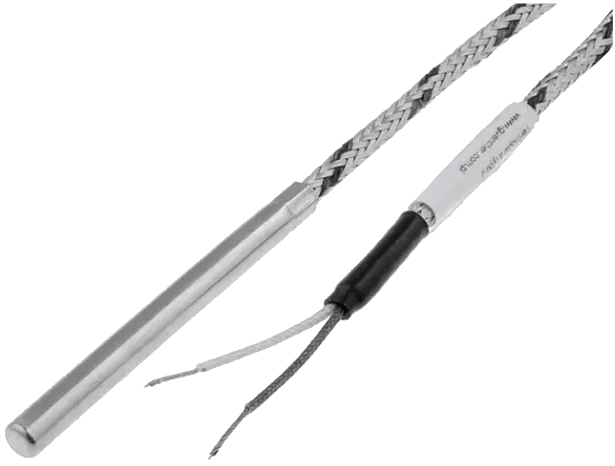
\includegraphics[width=0.4\textwidth]{images/termoclanek-72-21301041-k.png}
    \caption[Termočlánek 72-21301041 typu K.]{Termočlánek 72-21301041 typu K \cite{termoclanek-k}.}
    \label{fig:termoclanek-72-21301041-k}
\end{figure}

Na obrázku \ref{fig:vyrez-teplotni-senzory-zasobnik-otopne-vody} je výřez části z celkového nákresu (obrázek \ref{fig:otopna-soustava-a-elektronika-rez-domu}) pro umístění teplotních senzorů v zásobníku otopné vody. Pro snímání teplot z centrálního zásobníku otopné vody, venkovní teploty a~prostorových teplot z jednotlivých místností slouží teplotní senzor DS18B20 od výrobce Maxim. Umožňuje měřit v teplotním rozsahu od -55 °C do +125~°C. V~rozsahu od -10 °C do +85 °C měří s přesností ±0,5 °C. Senzor umožňuje měřit teplotu s přesností 12 bitů. Pro komunikaci využívá 1-Wire sběrnici (způsob komunikace je popsán v \ref{sec:1-wire-sbernice} v části 1-Wire sběrnice). Ve svém konkrétním řešením využívám senzory v pouzdře TO-92 pro nástěnné snímače prostorové teploty, pro centrální zásobník otopné vody a~venkovní teplotu je senzor uložen do ochranného pouzdra.

\subsection{Realizace 1-Wire sběrnice u zásobníku otopné vody}
\begin{figure}[H]
   \centering
   \def\svgwidth{0.2\columnwidth}
   \input{images/svg/otopna-soustava/vyrez-1-wire-sbernice-u-zasobniku-otopne-vody.pdf_tex}
   \caption[Výřez pro umístění sdružení 1-Wire sběrnice u zásobníku otopné vody.]{Výřez z obrázku \ref{fig:otopna-soustava-a-elektronika-rez-domu} – umístění sdružení 1-Wire sběrnice u zásobníku otopné vody.}
    \label{fig:vyrez-1-wire-sbernice-u-zasobniku-otopne-vody}
\end{figure}

Na obrázku \ref{fig:vyrez-1-wire-sbernice-u-zasobniku-otopne-vody} je výřez části z celkového nákresu (obrázek \ref{fig:otopna-soustava-a-elektronika-rez-domu}) pro sdružení 1-Wire sběrnice u zásobníku otopné vody. Na obrázku \ref{fig:dps-1-wire-sbernice-u-zasobniku-otopne-vody} je realizovaná DPS pro teplotní senzory u zásobníku otopné vody. Princip zapojení včetně ochrana na napájecí i datové části je popsán v~části \ref{sec:dps-se-vstupy-vystupy-pro-raspberry-pi} (datová část 1-Wire sběrnice). Na obrázku \ref{fig:instalacni-krabice-cidla-u-zasobniku-otopne-vody} je vidět horní část DPS vložená do instalační krabice. Celkově je zde k dispozici 6~pozic pro upevnění přes svorkovnice teplotní senzory. V současnosti jsou zde napojeny 3 teplotní senzory pro snímání teplot z horní, střední a~spodní části zásobníku otopné vody. Umístění senzorů je dáno výrobcem zásobníku a senzory jsou vloženy do dutiny. Samotná 1-Wire sběrnice je realizovaná pomocí UTP kabelu kategorie 5e. Na pinu číslo 4 jsou DATA, na pinu 5 je zem (GND) a na pinu 3 je napájení 5~V. Pro měření venkovní teploty je senzor DS18B20 v~pouzdře TO-92 připevněn na UTP kabel a zataven plastovou hmotou, na níž je následně nanesena smršťovací ochranná bužírka. Na obrázku \ref{fig:zasobnik-otopné-vody} jsou vyznačená místa s~umístěním teplotních senzorů. Celkové schéma zapojení je v příloze \ref{app:schemata-ostatni}.

\begin{figure}[H]
\centering
\begin{subfigure}{.5\textwidth}
    \centering
    \includegraphics[width=\textwidth]{images/zasobnik-otopne-vody/dps-1-wire-sbernice-u-zasobniku-otopne-vody.png}
    \caption{Realizovaná DPS pro teplotní senzory 1-Wire sběrnice u zásobníku otopné vody.}
    \label{fig:dps-1-wire-sbernice-u-zasobniku-otopne-vody}
\end{subfigure}%
\begin{subfigure}{.5\textwidth}
   	\centering
    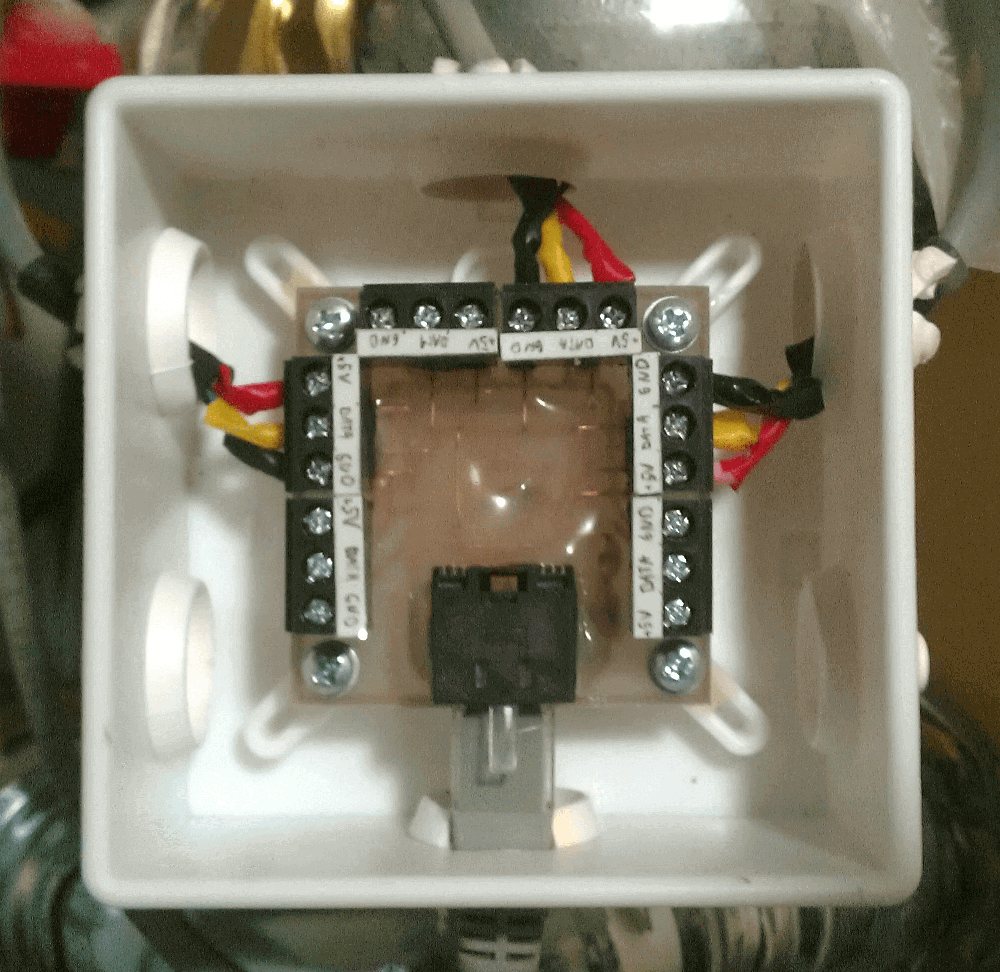
\includegraphics[width=0.95\textwidth]{images/zasobnik-otopne-vody/instalacni-krabice-cidla-u-zasobniku-otopne-vody.png}
    \caption{Horní část DPS umístěná do instalační krabice.}
    \label{fig:instalacni-krabice-cidla-u-zasobniku-otopne-vody}
\end{subfigure}%
\caption{Sdružení 1-Wire sběrnice u zásobníku otopné vody}
\end{figure}

%\begin{figure}[H]
%    \centering
%    \includegraphics[width=0.4\textwidth]{images/zasobnik-otopne-vody/ds18b20-ochrana.png}
%    \caption{Teplotní senzor DS18B20 v~ochranném pouzdře.}
%    \label{fig:ds18b20-ochrana}
%\end{figure}

\begin{figure}[H]
    \centering
    \includegraphics[width=0.85\textwidth]{images/zasobnik-otopne-vody/zasobnik-otopné-vody.png}
    \caption[Zásobník otopné vody.]{Zásobník otopné vody. Červené kroužky označují místa teplotních senzorů.}
    \label{fig:zasobnik-otopné-vody}
\end{figure}

\section{I$^2$C sběrnice}
\label{sec:i2c-sbernice}

\begin{figure}[H]
   \centering
    \def\svgwidth{0.3\columnwidth}
   \input{images/svg/otopna-soustava/vyrez-i2c-sbernice.pdf_tex}
    \caption[Výřez pro modul I$^2$C sběrnice u centrální jednotky.]{Výřez z obrázku \ref{fig:otopna-soustava-a-elektronika-rez-domu} – modul I$^2$C sběrnice u centrální jednotky.}
    \label{fig:vyrez-i2c-sbernice}
\end{figure}

Na obrázku \ref{fig:vyrez-i2c-sbernice} je výřez části z celkového nákresu (obrázek \ref{fig:otopna-soustava-a-elektronika-rez-domu}) pro modul I$^2$C sběrnici u centrální jednotky. Sběrnice I$^2$C je realizovaná pomocí zakoupeného modulu (obrázek \ref{fig:modul-pca9615}) s~obvodem PCA9615 \cite{vyrobce-pca9615} (blokové schéma je v příloze \ref{fig:blokove-schema-pca9615-i2c-sbernice}) do firmy  NXP Semiconductors. Vstupní signál SCL a~SDA je veden přímo z~centrální jednotky na vstupu obvodu PCA9615, napájení je s 3,3~V logikou. Výstup z PCA9615 je diferenciální signál. Napájení na této straně je 5 V. Sběrnice je realizovaná pomocí UTP kategorie 5e, výstup z~modulu je realizován pomocí konektoru RJ45. Vzhledem k použití UTP kabelu a diferenciálnímu přenosu je možné dosáhnout velké vzdálenosti sběrnice. Nejdelší bod dosahuje přibližně 30 m, je tedy možné použít I$^2$C sběrnici na vzdálenost, pro kterou není standartě dělána. Použitá frekvence je 100~kHz. Jedná se tedy o plnohodnotnou I$^2$C sběrnici. Důvodem pro zvolení této varianty bylo na základě výběru displeje s I$^2$C sběrnicí (jednoduché a~levné řešení), dále jedná se o klasické zapojení displeje jako by se nalézal v~krátké vzdálenosti od centrální jednotky a není tak nutný převod jako při využít např. RS485 na \acrshort{uart} (\textit{\acrlong{uart}}) a~následně na I$^2$C sběrnici, v neposlední řadě komunikace je definována podle protokolu I$^2$C.  Jeden modul se nalézá na straně centrální jednotky a pak na straně krbů. Napájení 5 V je realizováno pomocí samostatných kabelů, není tedy součástí UTP kabelu. Z důvodu omezení kabeláže je sběrnice realizována v jednom UTP kabelu s 1-Wire sběrnicí, tedy přesněji jsou využity volné vodiče 1,2 pro SCL a~7,~8 pro SDA. Zařízení lze zapojovat jak na straně před PCA9615, tak i~na diferenciální straně, je však výhodné připojené uzly udržet co v~nejkratší vzdálenosti kvůli degradování signálu. Blokové schéma je na obrázku \ref{fig:blokove-schema-pca9615-i2c-sbernice} včetně napojení uzlů. Schéma zapojení modulu v příloze \ref{app:schemata-ostatni}, upraveno z \cite{pca9615-schema-zapojeni}.


Výhodou PCA9615 je automatický výběr směru komunikace, není potřeba externí ovládání. Komunikace je možná až do rychlosti 1 MHz (přibližně pro 3 m), se zvýšenou délkou je však nutné rychlost snížit. Komunikace využívá standardní protokol I$^2$C. Koncová zařízení je možné napájet z různých zdrojů. V neposlední řadě se jedná o jednoduché řešení bez nutných další zařízení na straně Slave, stačí pouze zapojit koncové zařízení s~podporou I$^2$C. Na obrázku \ref{fig:modul-pca9615-transily} jsou pro větší ochranu modulu přidány obousměrné transil diody (SM6T6V8CAY \cite{sm6t6v8cay}) připájené na vstupní piny konektoru RJ45 (obvod sám o sobě poskytuje vstupní ochranu pro ESD). Pro rozbočení I$^2$C sběrnice do jednotlivých pater slouží DPS s konektory RJ45 (schéma viz příloha \ref{app:schemata-ostatni}, obrázky viz příloha \ref{app:rozbocovac-i2c}).

\begin{figure}[H]
\centering
\begin{subfigure}{.5\textwidth}
    \centering
    \includegraphics[width=0.5\textwidth]{images/krb/modul-pca9615-transily.png}
    \caption{Spodní strana s ochrannými transily.}
    \label{fig:modul-pca9615-transily}
\end{subfigure}%
\begin{subfigure}{.5\textwidth}
    \centering
    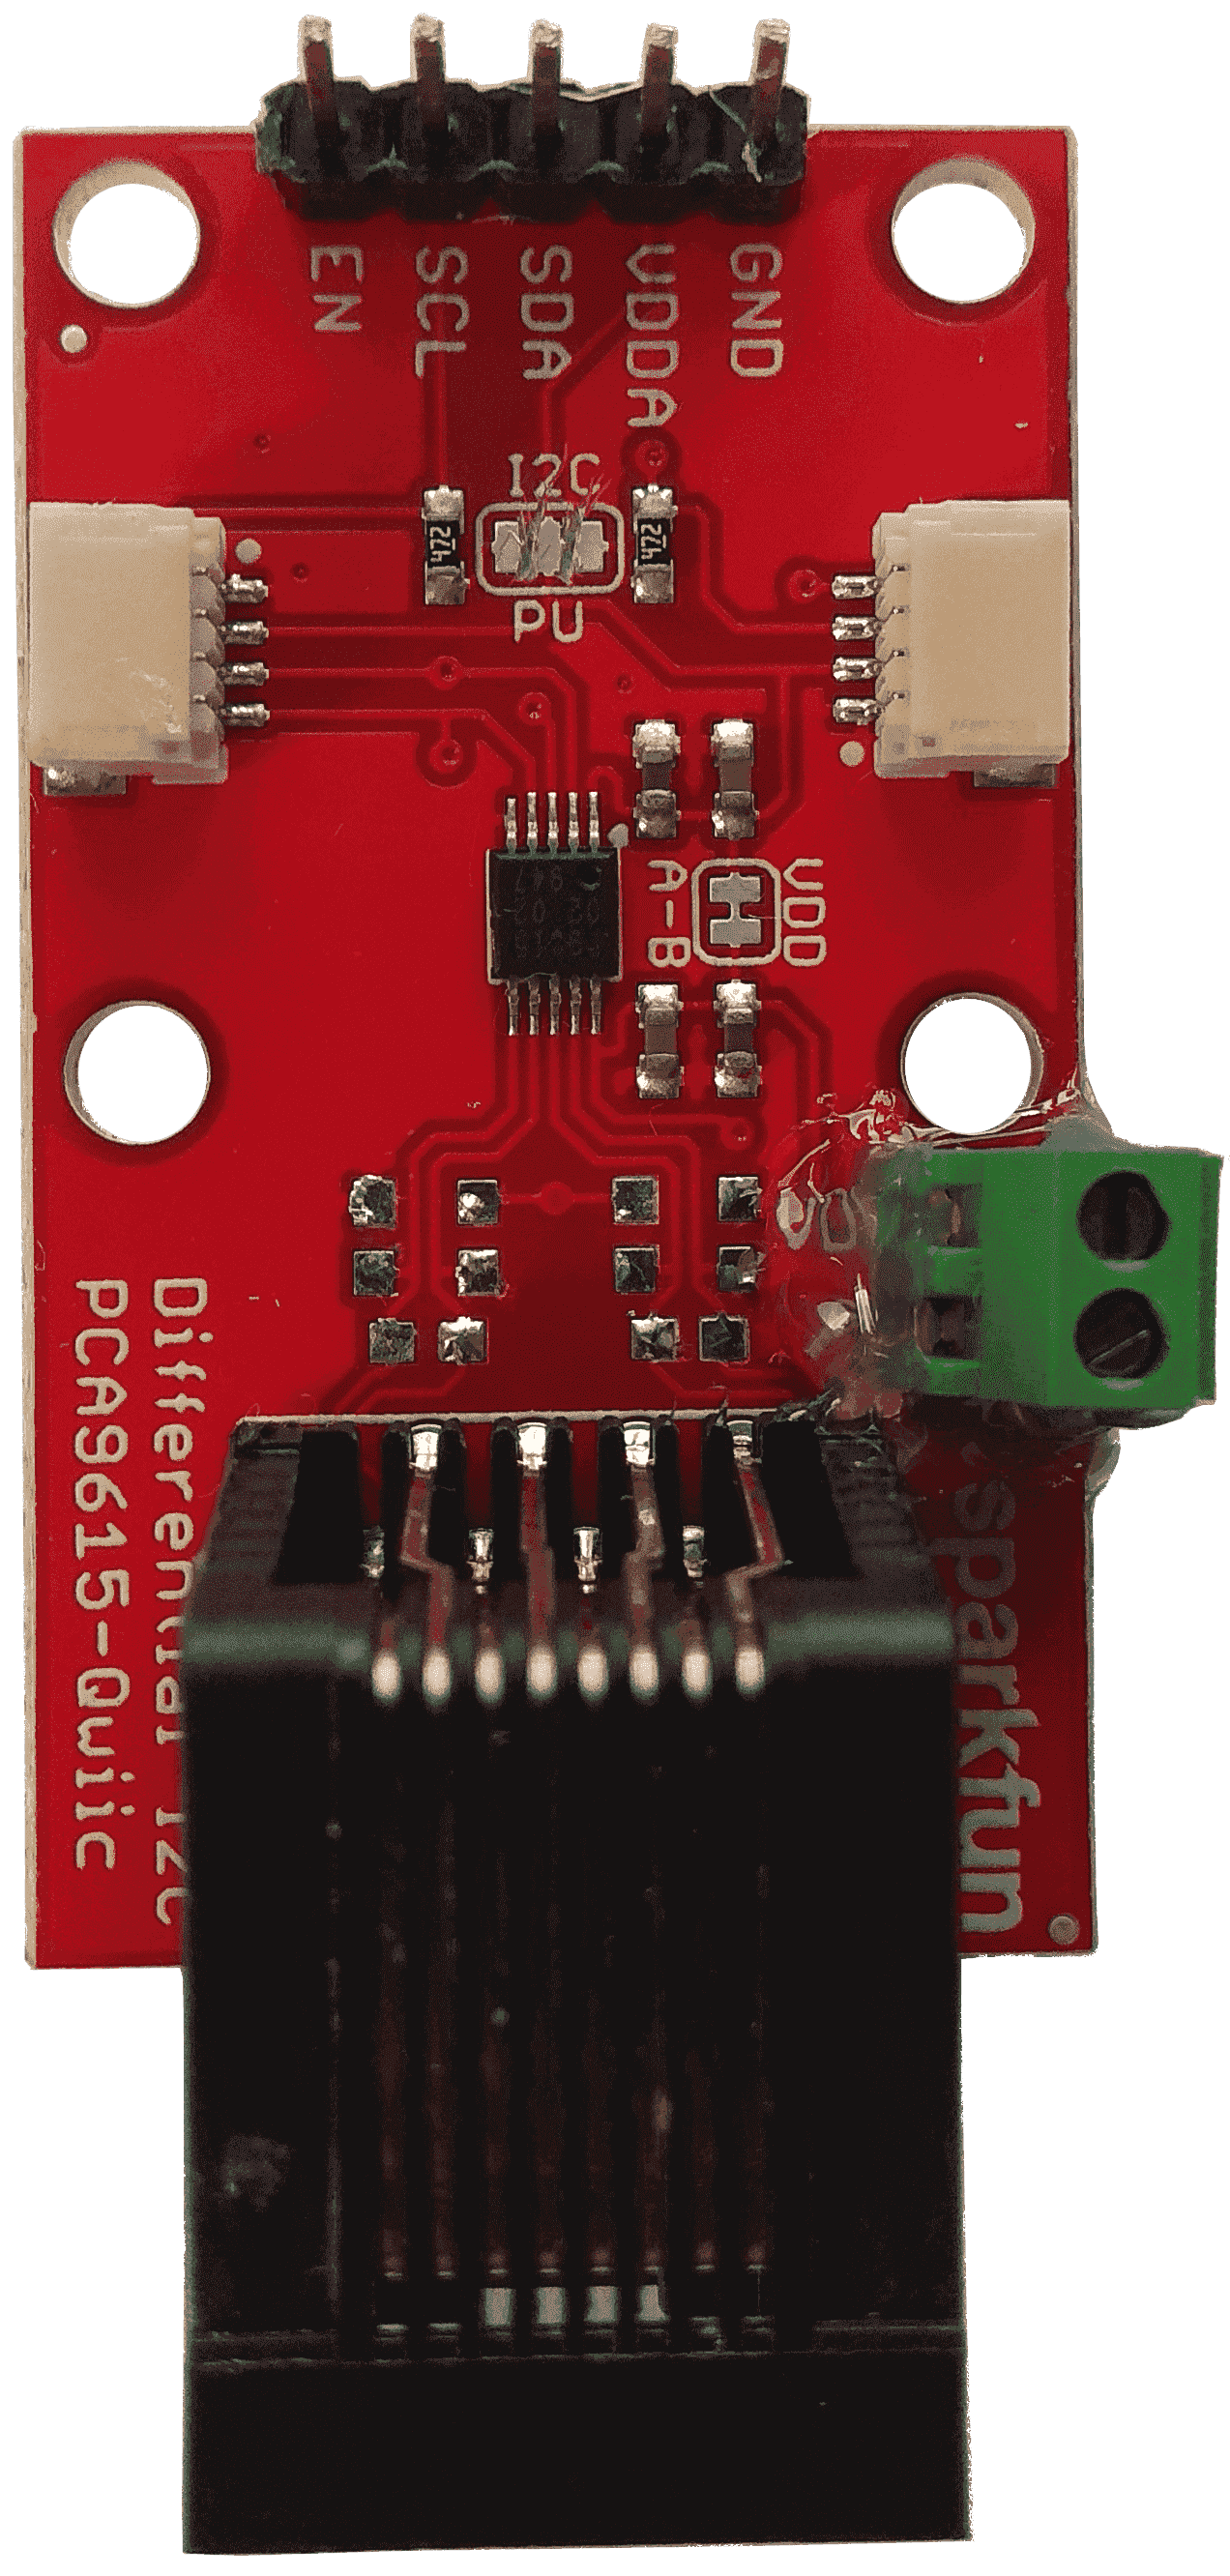
\includegraphics[width=0.45\textwidth]{images/krb/modul-pca9615-i2c-sbernice.png}
    \caption{Vrchní strana.}
    \label{fig:modul-pca9615-i2c-sbernice}
\end{subfigure}
\caption{Modul s obvodem PCA9615.}
\label{fig:modul-pca9615}
\end{figure}

\section{\acrshort{dps} se vstupy/výstupu pro Raspberry Pi}
\label{sec:dps-se-vstupy-vystupy-pro-raspberry-pi}

\subsubsection{Datová část 1-Wire sběrnici}
\label{sec:datova-cast-1-wire-sbernice}
Pro zmíněnou 1-Wire sběrnici jsou realizované ESD ochrany spočívající použití Zenerovy diody a  5 $\Omega$ rezistorů, všechny součástky jsou zaintegrované v~jednom pouzdře TSOC, integrovaný obvod je od výrobce Maxim s označením DS9503. Integrovaná Zenerova dioda má nízkou kapacitu desítky pF, tím pádem nepřispívá k nadměrnému kapacitnímu zatěžování sběrnice. Omezovací rezistory slouží k omezení proudu při přepěťovém napěťovém impulzu pro ochranu Zenerovy diody (když je otevřena) před nadměrným proudem během ESD události, při běžné komunikace jsou zanedbatelné. Upínací napětí Zenerovy diody je 5,5 V při 0,9 A (průrazné napětí je přibližně 11 V) během ESD události. Dále je zde zařazena TVS dioda (ESD9L5.0ST5G) s upínacím napětí maximálně 9,8 V při 1 A, slouží jako sekundární ochrana pokud by selhala část s DS9503. 

Další možností je použití galvanického oddělení především pomocí optočlenu. Zde však nastává problém s obousměrnou poloduplexní komunikací, je potřeba zajistit komunikaci oběma směry. Optočleny vkládání zpoždění, které by podle specifikace 1-Wire sběrnice nemělo přesáhnout 1 $\mu$ s. Dále je potřeba oddělený převodník napětí či samotný zdroj pro napájení oddělených částí optočlenu a~další potřebné externí součástky. V neposlední řadě je nutné, alespoň podle výrobce Maxim použít převodník UART na 1-Wire či I$^2$C na 1-Wire sběrnici. Řešení pomocí galvanického oddělení ve výsledku zesložiťuje řešení a též prodražuje. Vzhledem k domácímu nasazení jsem se rozhodl zvolit variantu podle obrázku~\ref{fig:ochrany-1-wire}.

Vzhledem k toleranci napěťové úrovně 3,3 V pro piny u Raspberry Pi, je navržen obousměrný převodník napěťových úrovní z 3,3 V na 5~V a opačně, realizovaný pomocí MOSFET tranzistoru (BSS138P), pull-up rezistorů.

Na obrázku \ref{fig:ochrany-1-wire} jsou vidět dvě větve pro 1-Wire sběrnici, je to z důvodu dvou typů zařízení, teplotních čidel DS18B20 a  zesilovače s termočlánkem, které mají různé časování, popsáno více níže. Sběrnici, lze sdružit do jedné pomocí propojky P6.

\begin{figure}[H]
    \centering
    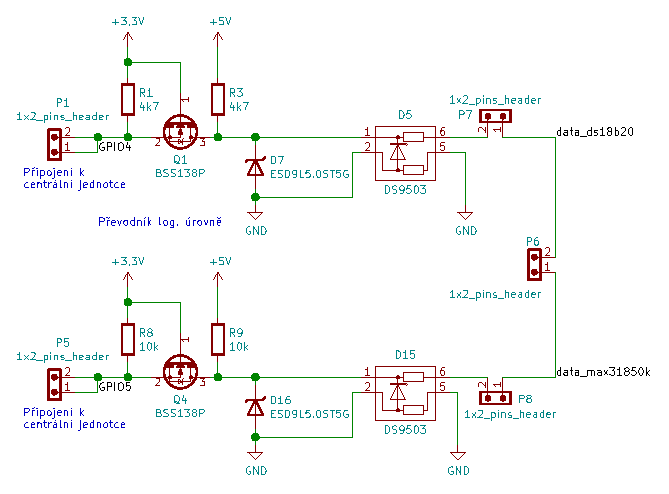
\includegraphics[width=\textwidth]{images/svg/kicad/ochrany-1-wire.eps}
    \caption[ESD ochrany pro 1-Wire sběrnici s~převodním napěťových úrovní]{ESD ochrany pro 1-Wire sběrnici s převodním napěťových úrovní. Kolíková lišta P1, P5 je připojena na Raspberry Pi.}
    \label{fig:ochrany-1-wire}
\end{figure}


\subsubsection{Napájení 1-Wire sběrnice}
\label{sec:napajeni-1-wire-sbernice}
Pro ochranu napájení 1-Wire sběrnice (5 V) jsou veškerá koncové teplotní senzory napájené přes elektronickou pojistku od Texas Instrumenst s označením TPS2600, obrázek \ref{fig:ochrana-napajeni-1-wire}. Která zajišťuje ochranu pro vstupní napětí, hlídá maximální hodnotu vstupního napětí do nastavené meze 5,25 V (maximální hranice je 60 V), minimální vstupní napětí do nastavené meze 4,75 V (minimální hranice je -60 V). Vstupní omezení napětí je pomocí rezistorů R5, R10, R11 a R12. Omezovací proud je nastaven na přibližně 73 mA (hodnotu lze změnit přes potenciometr R17), při jeho překročení dojde k odpojení výstupu pod dobu dokud nedojde k odstranění závady. Kondenzátor C2 nastavuje rychlost náběhu výstupního napětí. Pro indikaci chyb napájení je červená LED.

\begin{figure}[H]
    \centering
    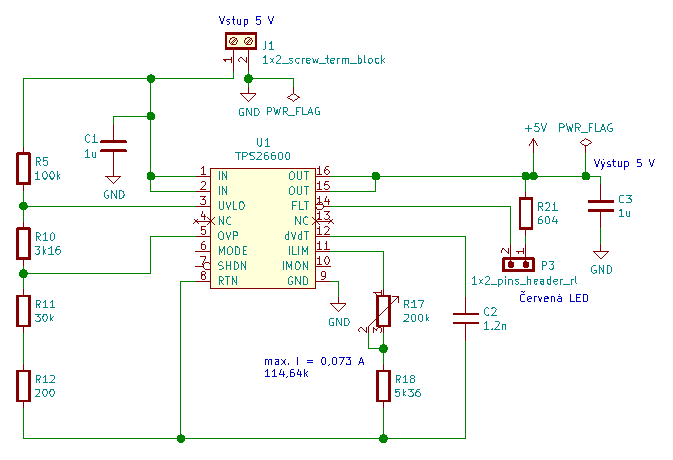
\includegraphics[width=\textwidth]{images/svg/kicad/ochrana-napajeni-1-wire.eps}
    \caption{Obvod TPS26600 pro ochranu napájení 1-Wire sběrnice.}
    \label{fig:ochrana-napajeni-1-wire}
\end{figure}

\subsubsection{Ochrana pro chodbové nástěnné termostaty}
Obdobně jako v části \ref{sec:datova-cast-1-wire-sbernice} (datová část 1-Wire sběrnice) je stejná ochrana pro snímání logické úrovně z~chodbových nástěnných termostatů. Při sepnutí chodbového termostatu na daném patře je detekována log. 0 (požadavek na vytápění) v opačném případě je zde log. 1 (zastavení vytápění). Chodbové nástěnné termostaty jsou popsány v sekci \ref{sec:digitalni-chodbove-termostaty}.

\subsubsection{Ochrana napájení 3,3 V}
Přímo z Raspberry Pi je využito napětí 3,3 V pro převodník napětí, popsaný v~části \ref{sec:datova-cast-1-wire-sbernice} (datová část 1-Wire sběrnice). Zde je použita vratná pojistka polymerový PTC (RXEF005) se spínacím proudem 100 mA, pro omezení proudu v~případě poruchy, dále je zde transilová dioda (SM2T3V3A) pro ochranu při přepětí (s~upínacím napětí max. 6,5 V (při 25 A, 10/1000~µs), průrazné napětí 3,6 V). Na obrázku \ref{fig:ochrana-napajeni-3_3-v} je zobrazena popsaná ochrana.

\begin{figure}[H]
    \centering
    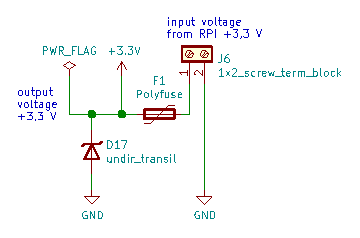
\includegraphics[width=0.6\textwidth]{images/svg/kicad/ochrana-napajeni-3_3-v.eps}
    \caption{Ochrana pro napájení 3,3 V z~Raspberry Pi.}
    \label{fig:ochrana-napajeni-3_3-v}
\end{figure}

\subsubsection{Způsob realizace 1-Wire sběrnice}
Samotná 1-Wire sběrnice je realizovaná pomocí UTP kabelu kategorie Cat5e. Na pinu číslo 4 jsou DATA, na pinu 5 je zem (GND) a na pinu 3 je napájení 5~V. Ze samotné DPS je sběrnice vyvedena pomocí konektorů RJ45, čtyři konektory pro teplotní senzory DS18B20 a čtyři pro termočlánky s MAX31850K.

\subsubsection{Realizovaná DPS ochran pro centrální jednotku Raspberry Pi}
Na obrázku \ref{fig:dps-rpi-1-wire-termostaty-ochrany-spodek} a \ref{fig:dps-rpi-1-wire-termostaty-ochrany-vrsek} je realizovaná DPS vstupů/výstupů pro centrální jednotku Raspberry Pi. Deska byla vlastnoručně navržena, vyrobena a osazena. Je aplikován ochranný lak, na vrchní propojky byl též aplikován ochranný lak a následně zakryty tavnou plastovou hmotou. Celkové schéma zapojení je v příloze \ref{app:schemata-ostatni}. Toto zařízení bylo realizováno jednou a je umístěné v rozvaděči.

\begin{figure}[H]
    \centering
    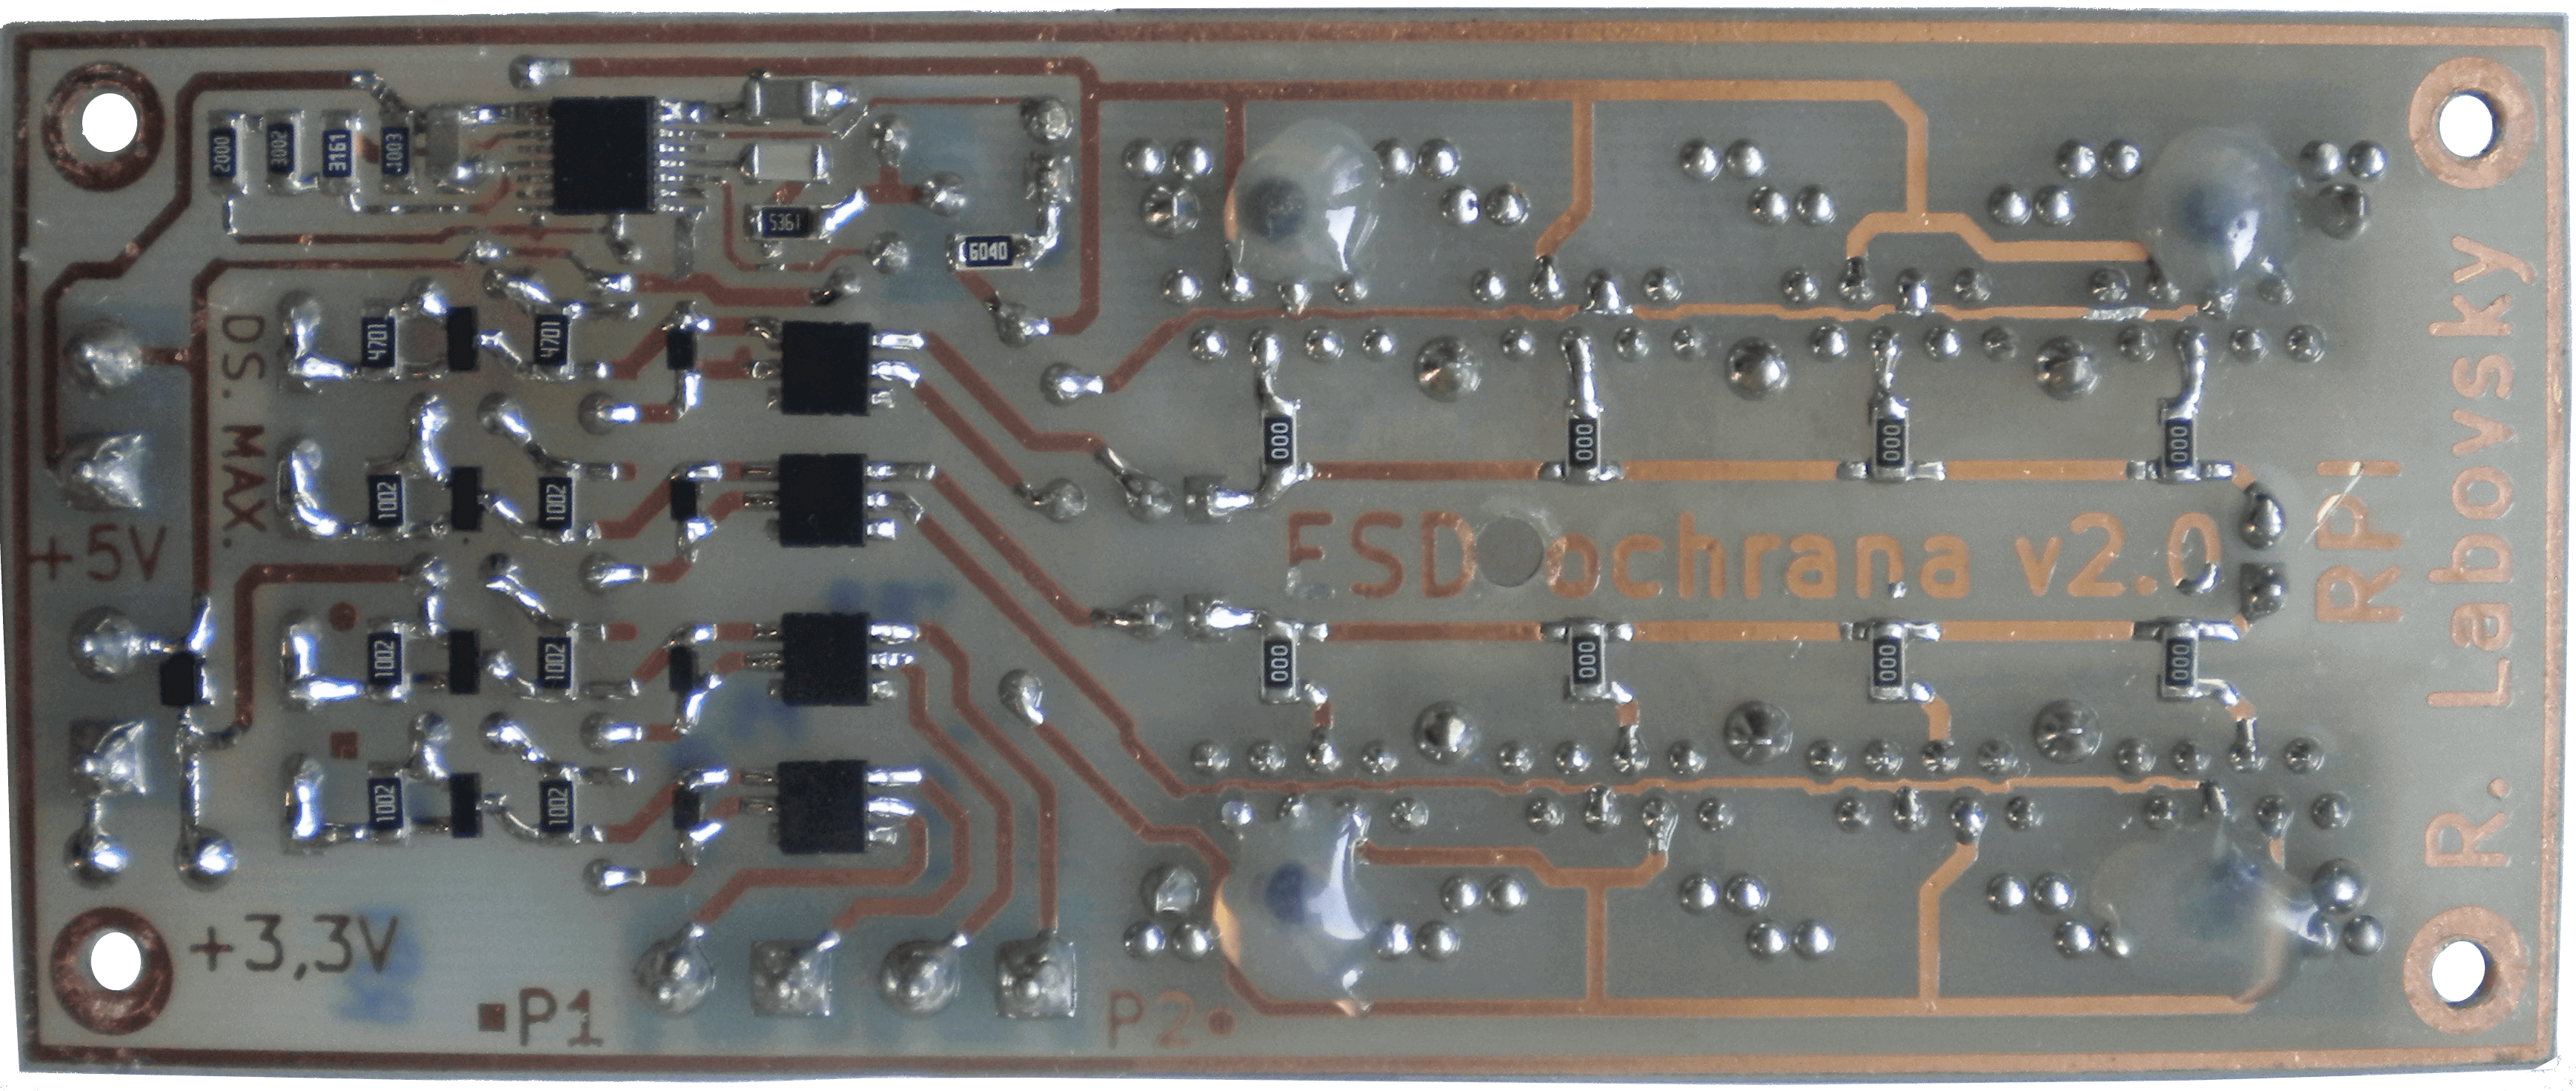
\includegraphics[width=\textwidth]{images/dps-rpi-1-wire-termostaty-ochrany-spodek.png}
    \caption{Spodní část DPS pro ochranu vstupů/výstupů pro centrální jednotku Raspberry Pi.}
    \label{fig:dps-rpi-1-wire-termostaty-ochrany-spodek}
\end{figure}

\begin{figure}[H]
    \centering
    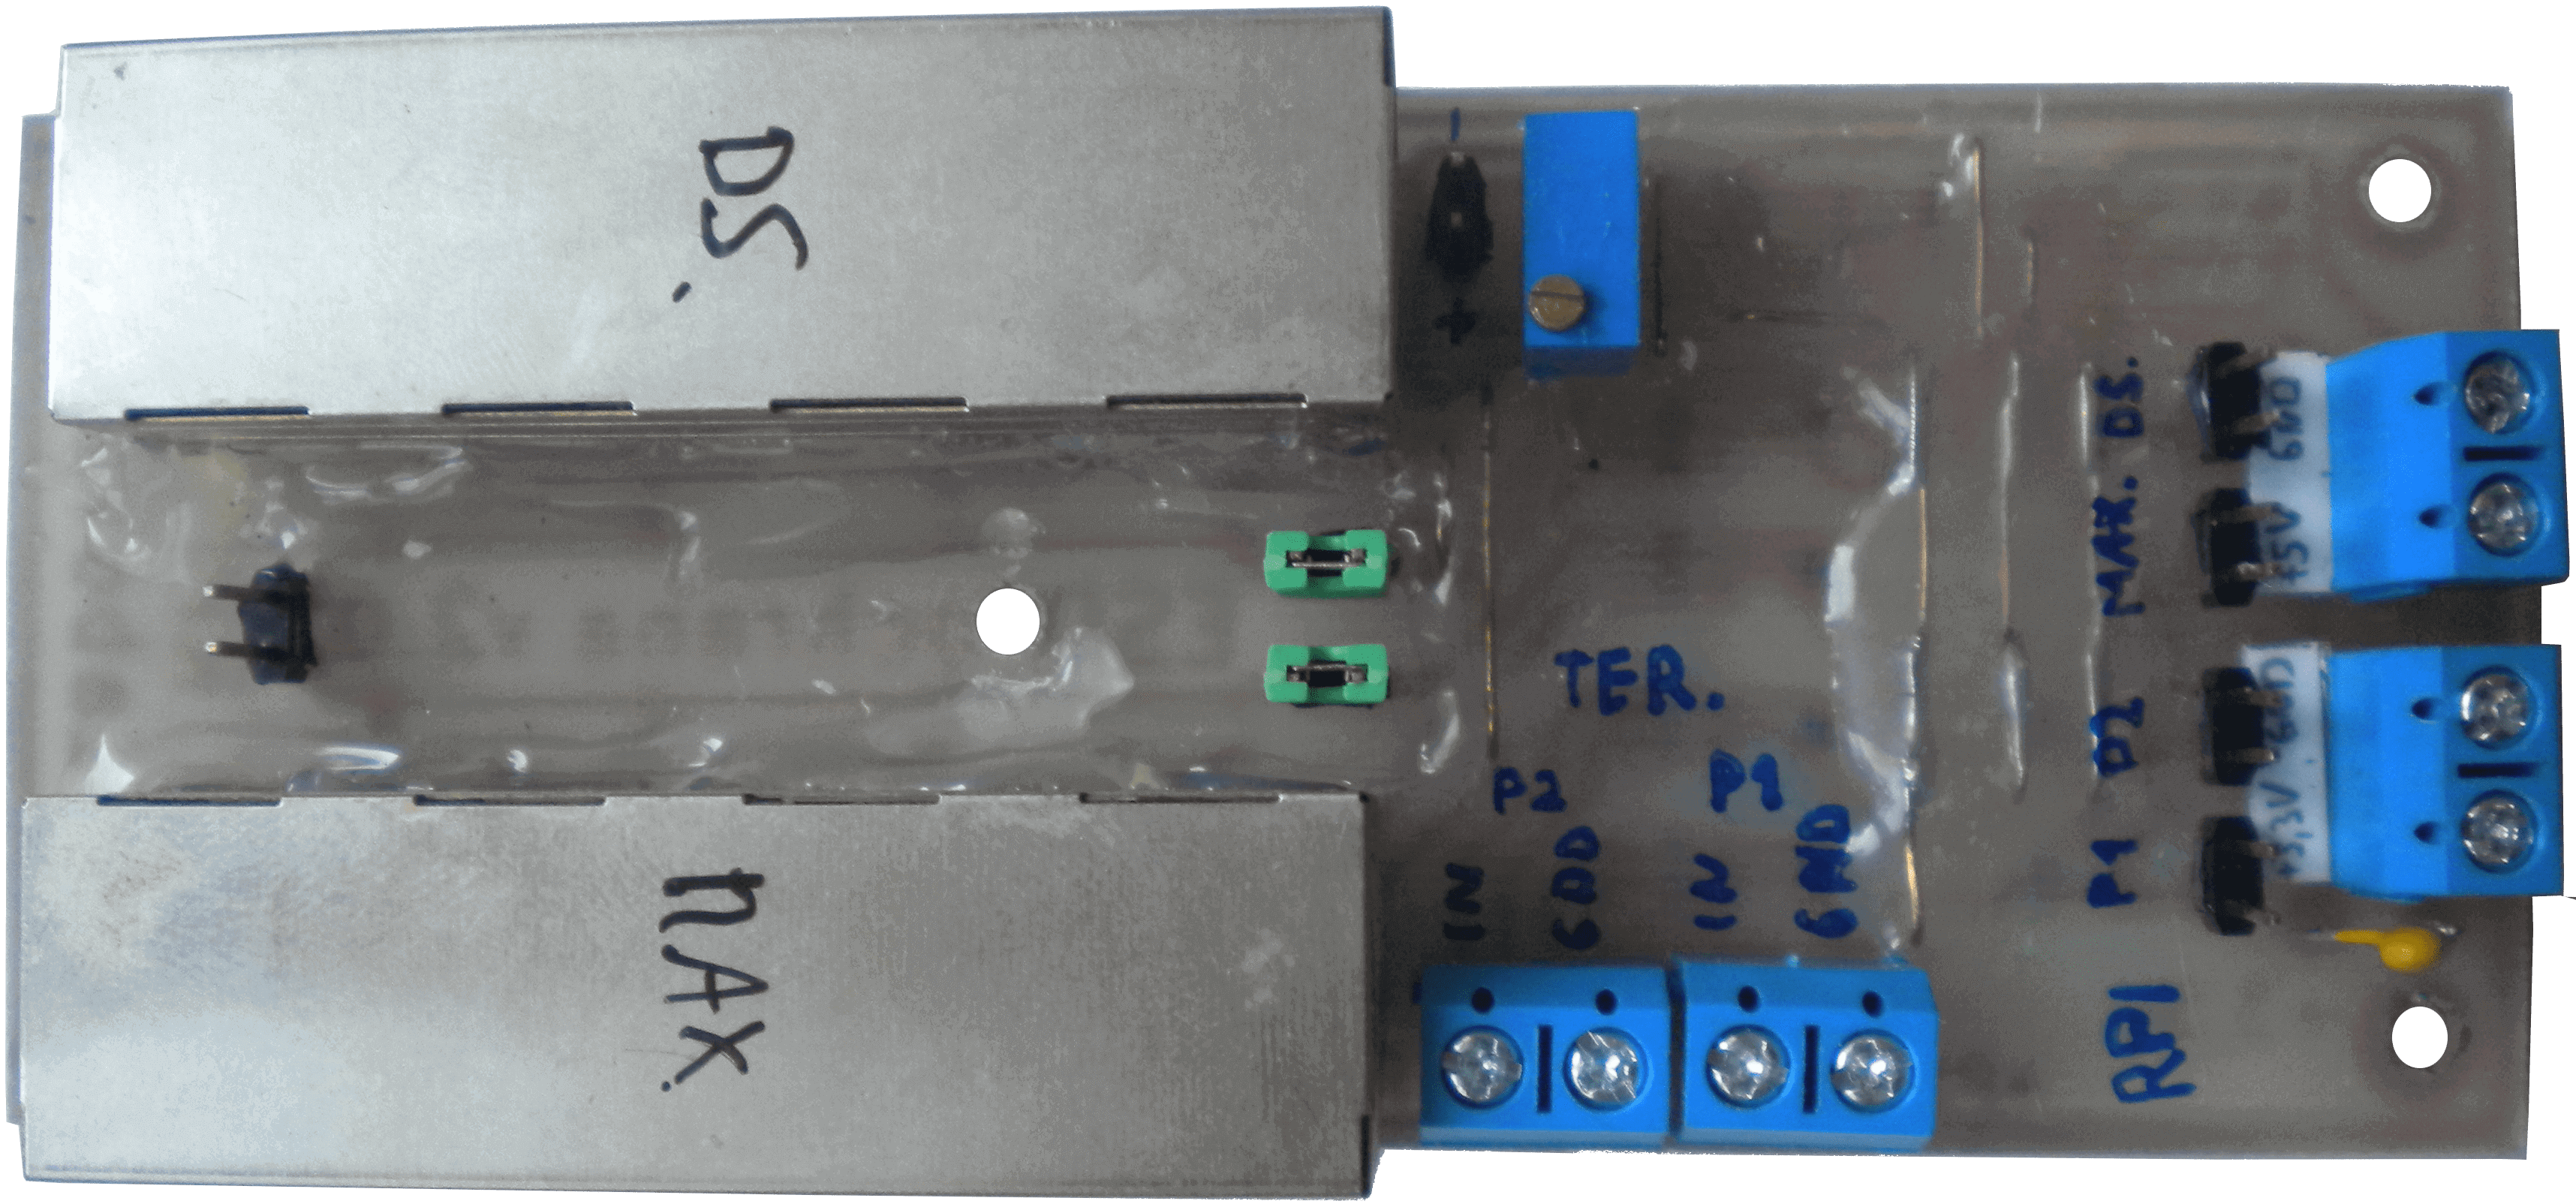
\includegraphics[width=\textwidth]{images/dps-rpi-1-wire-termostaty-ochrany-vrsek.png}
    \caption{Vrchní část DPS pro ochranu vstupů/výstupů pro Raspberry Pi.}
    \label{fig:dps-rpi-1-wire-termostaty-ochrany-vrsek}
\end{figure}

\section{DPS u krbů}
Navržená DPS se skládá z části elektronické pojistky TPS2600, zapojení je obdobné jako v \ref{sec:napajeni-1-wire-sbernice} (napájení 1-Wire sběrnice), navíc je na vstupu připojena transilová dioda (ESD9L5.0ST5G). Napěťové meze jsou nastaveny stejně, tedy minimální napětí je 4,75 V, maximální 5,25 V, proud je omezen na maximální hodnotu 100 mA. Dále je zde přivedena 1-Wire sběrnice přes konektor RJ45 s~obdobnými ochranami jako v \ref{sec:datova-cast-1-wire-sbernice} (datová část 1-Wire sběrnice), včetně stejných ochran pro napájení, pro připojení MAX31850K přes svorkovnici. V neposlední řadě jsou zde vstupy pro ovládání třech LED pro signalizaci (obrázek \ref{fig:led-indikace}) naakumulovaného zásobníku otopné vody, modrá led signalizuje stav horní části zásobníku, oranžová LED je pro střední část, červená je pro signalizaci spodní části. Vstupní část je chráněná přes DS9503 a transilovou diodou (ESD9L5.0ST5G). Sepnutí LED je přes tranzistor (BSS138P). Obdobně jsou řešeny oranžová a modrá LED. Celkové schéma zapojení je v příloze \ref{app:schemata-ostatni}.

\begin{figure}[H]
    \centering
    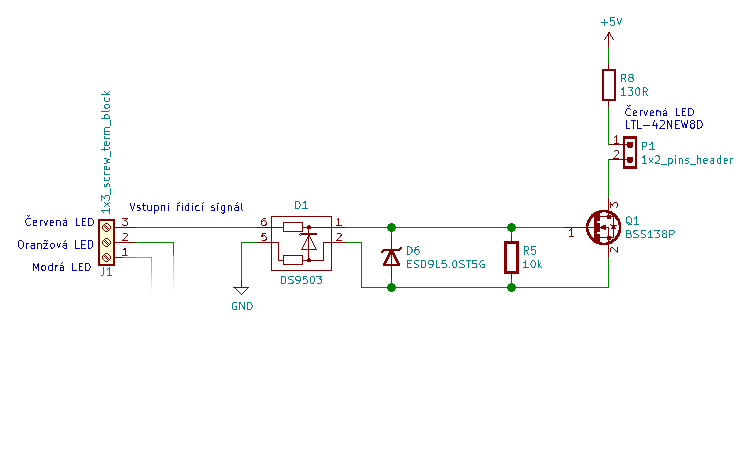
\includegraphics[width=\textwidth]{images/svg/kicad/led-indikace.eps}
    \caption{Zapojení pro ovládání signalizační červené LED.}
    \label{fig:led-indikace}
\end{figure}

\subsubsection{I$^2$C sběrnice}
\label{ses:i2c-sbernice}
Sběrnice I$^2$C je realizovaná pomocí zakoupeného modulu (obrázek \ref{fig:modul-pca9615-i2c-sbernice}) s~obvodem PCA9615 do firmy  NXP Semiconductors. Vstupní signál SCL a~SDA je veden přímo z~centrální jednotky na vstupu obovodu PCA9615, napájení je s 3,3 V logikou. Výstup z PCA9615 je pomocí diferenciální vedení, pro každý signál SCL a~SDA jsou použity dva vodiče. Napájení na této straně je pomocí 5 V. Sběrnice je realizovaná pomocí UTP Cat5e, výstup z~modulu je realizován pomocí konektoru RJ45. Vzhledem k použití UTP kabelu a diferenciálnímu přenosu je možné dosáhnout velké vzdálenosti sběrnice. Nejdelší bod dosahuje přibližně 30 m, je tedy možné použít I$^2$C sběrnici na vzdálenost pro kterou není standartě dělána. Použitá frekvence je 100~kHz. Jedná se tedy o plnohodnotnou I$^2$C sběrnici. Důvodem pro zvolení této varianty bylo na základě výběru displeje s I$^2$C sběrnicí (jednoduché a~levné řešení), dále jedná se o klasické zapojení displeje jako by se nalézal v~krátké vzdálenosti od centrální jednotky a není tak nutný převod jako při využít např. RS485 na UART a následně na I$^2$C sběrnici, v neposlední řadě komunikace je definována podle protokolu I$^2$C.  Jeden modul se nalézá na straně centrální jednotky a pak na straně krbů. Napájení 5 V je realizováno pomocí samostatných kabelů, není tedy součástí UTP kabelu. Z důvodu omezení kabeláže je sběrnice realizována v jednom UTP kabelu s 1-Wire sběrnicí, tedy přesněji jsou využity volné vodiče s číslem 1,2 pro SCL a 7,~8 pro SDA. Zařízení lze zapojovat jak na straně před PCA9615, tak i~na diferenciální straně, je však výhodné připojené uzly udržet co v nejkratší vzdálenosti kvůli degradování výkonu. Blokové schéma je na obrázku \ref{fig:blokove-schema-pca9615-i2c-sbernice} včetně napojení uzlů. Schéma zapojení modulu je na obrázku \ref{fig:zapojeni-pca9615-i2c-sbernice}.

\begin{figure}[H]
    \centering
    \def\svgwidth{\columnwidth}
    \input{images/svg/blokove-schema-pca9615-i2c-sbernice.pdf_tex}
    \caption[Blokové schéma zapojení obvodu PCA9615.]{Blokové schéma zapojení obvodu PCA9615 s impedančním zakončením sběrnice a možnostmi napojení uzlů. Upraveno z \cite{pca9615-schema-zapojeni}.}
    \label{fig:blokove-schema-pca9615-i2c-sbernice}
\end{figure}

\begin{figure}[H]
    \centering
    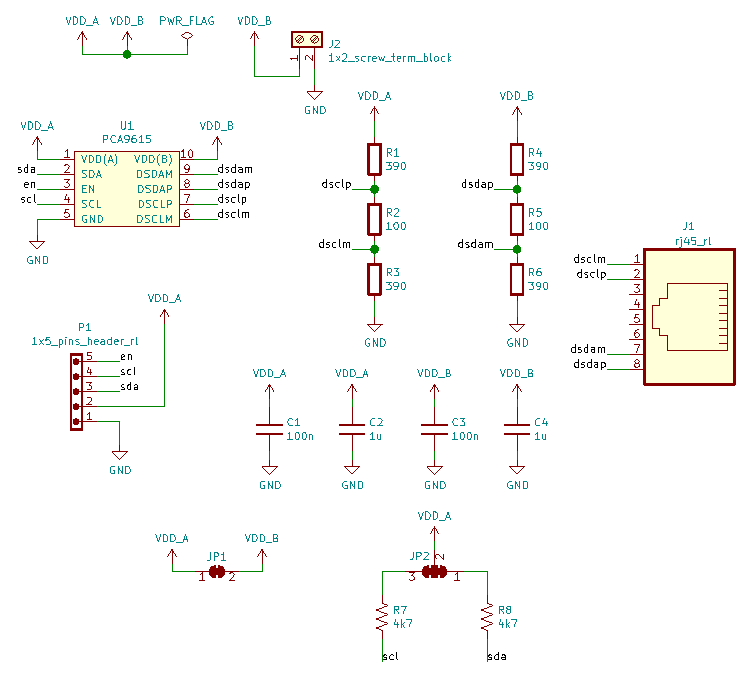
\includegraphics[width=\textwidth]{images/svg/kicad/zapojeni-pca9615-i2c-sbernice.eps}
    \caption[Zapojení PCA9615 v modulu.]{Zapojení PCA9615 v modulu. Upraveno z \cite{pca9615-schema-zapojeni}.}
    \label{fig:zapojeni-pca9615-i2c-sbernice}
\end{figure}

Výhodou PCA9615 je automatický výběr směru komunikace, není potřeba externího ovládání. Komunikace je možná až do rychlosti 1 MHz (přibližně pro 3 m), se zvýšenou délkou je však nutné rychlost snížit. Komunikace využívá standardního protokolu I$^2$C. ESD ochrana, v případě naindukování přepětí po cestě. Nezávislost napájení, je možné napájet koncová zařízení z jiného zdroje než Master. V neposlední řadě se jedná o jednoduché řešení bez nutných další zařízení na straně Slave, stačí pouze zapojit koncové zařízení s~podporou I$^2$C. Na obrázku \ref{fig:modul-pca9615-transily} jsou pro větší ochranu modulu přidány obousměrné transil diody (SM6T6V8CAY) připájené na vstupní piny konektoru RJ45.

\begin{figure}[H]
    \centering
    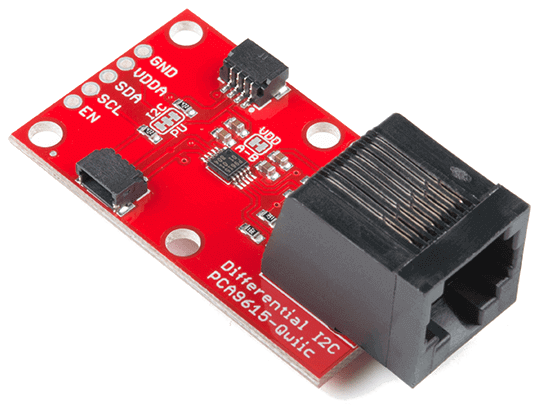
\includegraphics[width=0.6\textwidth]{images/modul-pca9615/modul-pca9615-i2c-sbernice.png}
    \caption[Modul s obvodem PCA9615.]{Modul s obvodem PCA9615 \cite{pca9615-i2c-modul}.}
    \label{fig:modul-pca9615-i2c-sbernice}
\end{figure}

\begin{figure}[H]
    \centering
    \includegraphics[width=0.6\textwidth]{images/modul-pca9615/modul-pca9615-transily.png}
    \caption[Modul s obvodem PCA9615 s transily.]{Modul s obvodem PCA9615 s ochrannými transily.}
    \label{fig:modul-pca9615-transily}
\end{figure}

\subsubsection{Měření teploty pomocí termočlánku a převodníku MAX31850K}
Teplotní senzory připojené na kouřovody krbů jsou realizované pomocí termočlánku z \ref{sec:teplotni-senzory-pro-krby}. Termočlánky jsou připojené k zakoupenému modulu (obrázek~\ref{fig:modul-max31850k-1-wire-prevodnik-termoclanku}) se zesilovačem napětí generované termočlánkem, hodnota napětí je následně převedena do digitální podoby včetně teplotní kompenzace studeného konce termočlánku a~tato hodnota je posílaná po 1-Wire sběrnici. Je možné připojit termočlánky typu K, J, N, S, R nebo E. Převodník umožňuje měřit teplotu s převodem pomocí AD převodníku až na 14 bitů. Rozlišení teploty činí 0,25 °C. Při teplotách -200 °C až 700 °C činí přesnost měřené teploty ±2~°C. Obvod disponuje detekcí zkratu (na GND nebo napájení) na vstupu pro termočlánek. Dále je zde detekci odpojeného termočlánku. Schéma zapojení modulu je na obrázku \ref{fig:zapojeni-max31850k-1-wire-prevodnik-termoclanku}.

\begin{figure}[H]
    \centering
    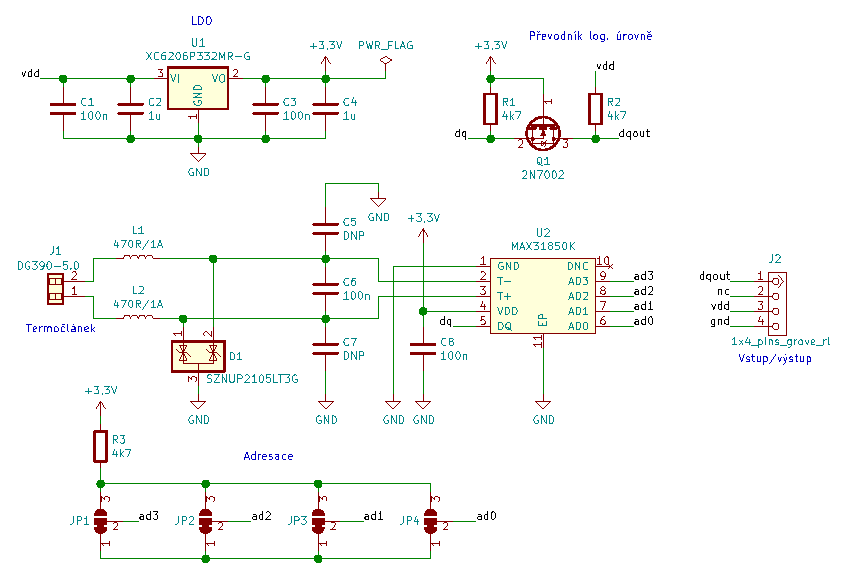
\includegraphics[width=\textwidth]{images/svg/kicad/zapojeni-max31850k-1-wire-prevodnik-termoclanku.eps}
    \caption[Zapojení MAX31850K v modulu.]{Zapojení MAX31850K v modulu. Upraveno z \cite{prevodnik-max31850k}.}
    \label{fig:zapojeni-max31850k-1-wire-prevodnik-termoclanku}
\end{figure}

\begin{figure}[H]
    \centering
    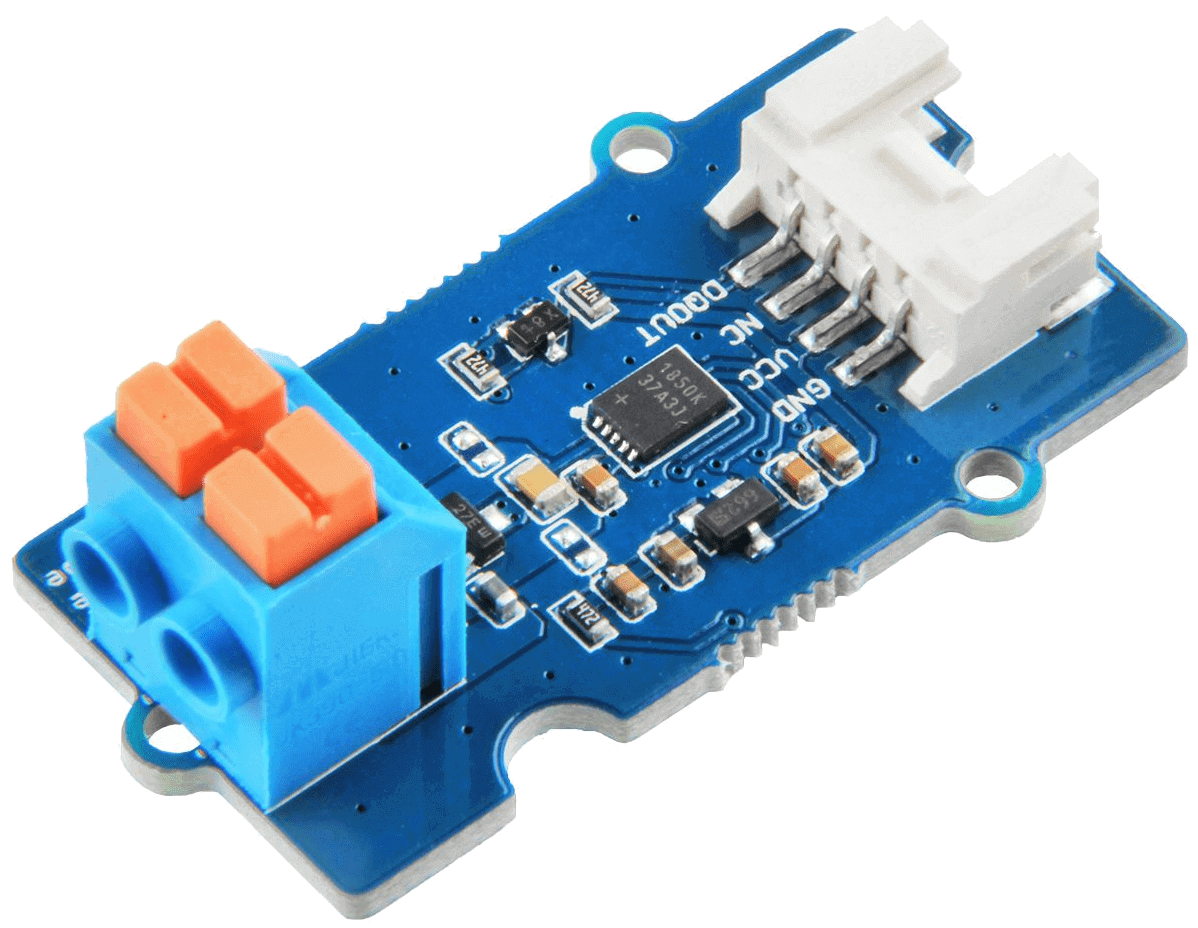
\includegraphics[width=0.6\textwidth]{images/modul-max31850k-1-wire-prevodnik-termoclanku.png}
    \caption[Modul s obvodem MAX31850K.]{Modul s obvodem MAX31850K \cite{prevodnik-max31850k}.}
    \label{fig:modul-max31850k-1-wire-prevodnik-termoclanku}
\end{figure}

\subsubsection{Realizace 1-Wire sběrnice u zásobníku otopné vody}
Na obrázku \ref{fig:dps-1-wire-sbernice-u-zasobniku-otopne-vody} je realizovaná DPS pro teplotní senzory u zásobníku otopné vody. Princip zapojení včetně ochrana na napájecí i datové části je popsán v~části \ref{sec:dps-se-vstupy-vystupy-pro-raspberry-pi} (datová část 1-Wire sběrnice). Na obrázku \ref{fig:instalacni-krabice-cidla-u-zasobniku-otopne-vody} je vidět horní část DPS vložená do instalační krabice. Celkově je zde k dispozici 6 pozic pro upevnění přes svorkovnice teplotní senzory. V současnosti jsou zde napojeny pouze 3 teplotní senzory (pro snímání teplot z horní, střední a spodní části zásobníku otopné vody). Na obrázku \ref{fig:ds18b20-ochrana} je teplotní senzor DS18B20 v~pouzdře TO-92 připevněn na UTP kabel a zataven plastovou hmotou na níž je následně nanesena smršťovací ochranná bužírka. Na obrázku \ref{fig:zasobnik-otopné-vody} jsou vyznačená místa s umístěním teplotních senzorů. Celkové schéma zapojení je v příloze \ref{app:schemata-ostatni}.

\begin{figure}[H]
    \centering
    \includegraphics[width=0.6\textwidth]{images/dps-1-wire-sbernice-u-zasobniku-otopne-vody.png}
    \caption{Realizovaná DPS pro teplotní senzory 1-Wire sběrnice u zásobníku otopné vody.}
    \label{fig:dps-1-wire-sbernice-u-zasobniku-otopne-vody}
\end{figure}

\begin{figure}[H]
    \centering
    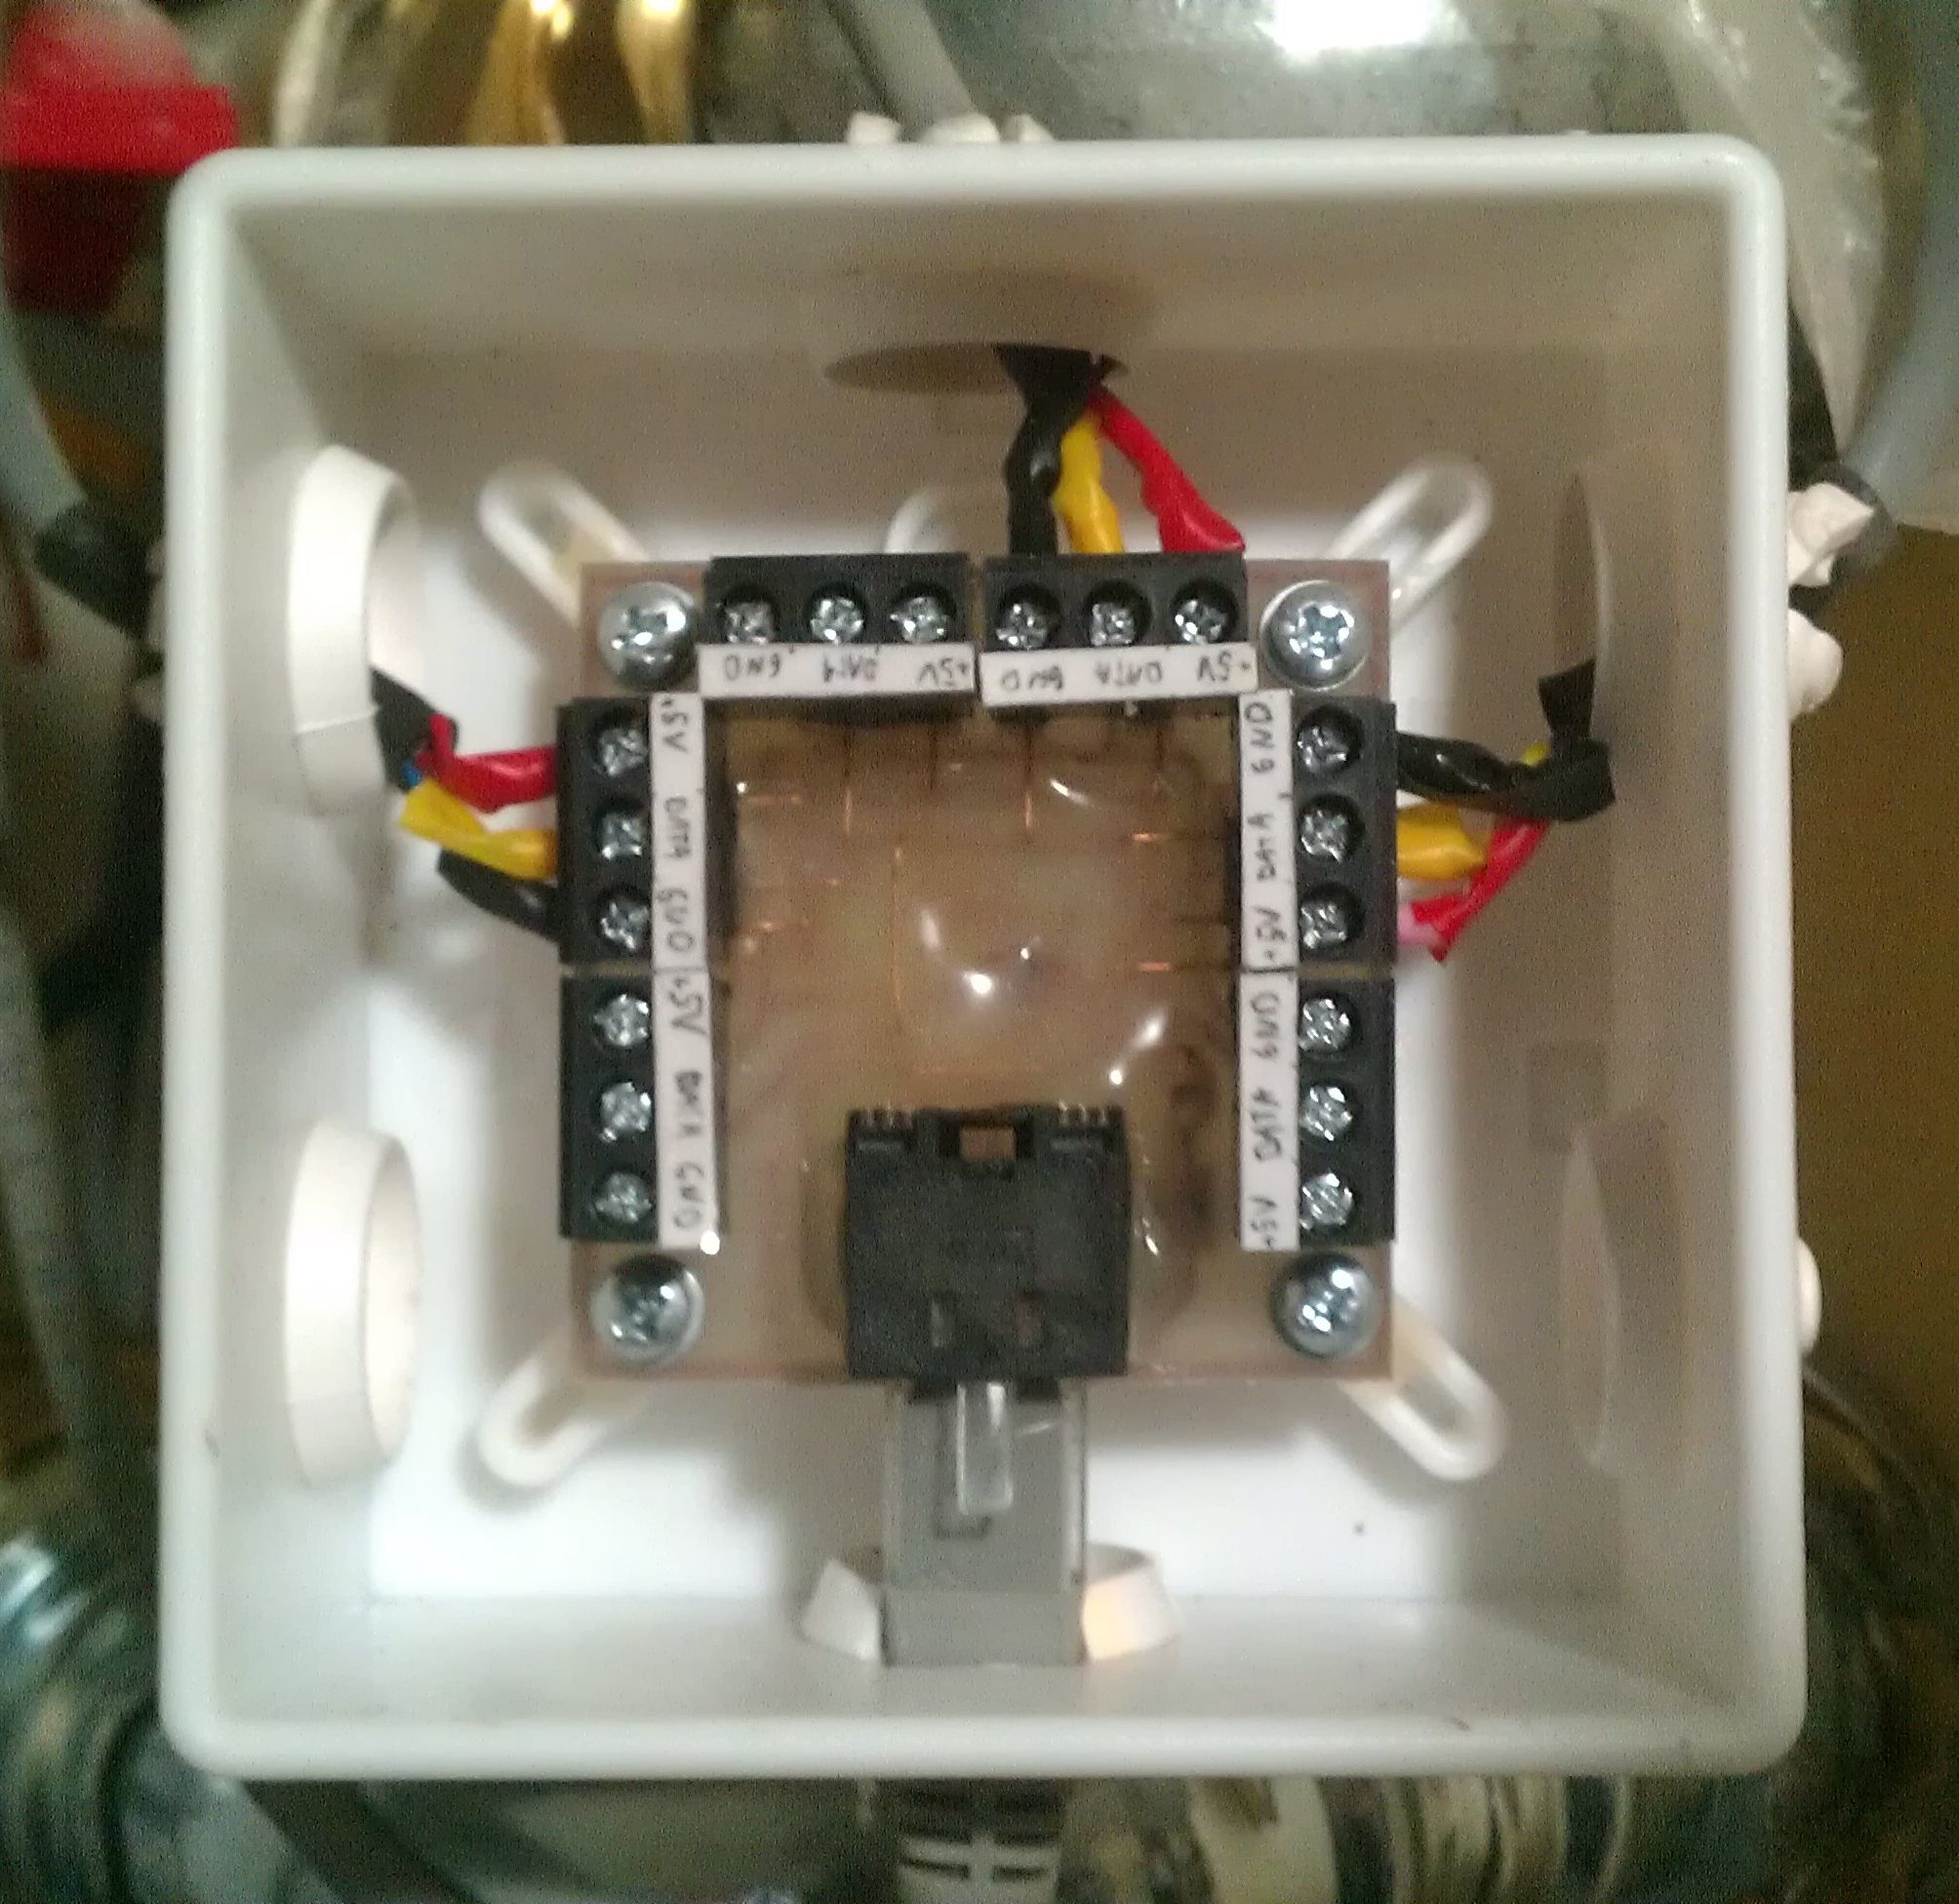
\includegraphics[width=0.6\textwidth]{images/instalacni-krabice-cidla-u-zasobniku-otopne-vody.png}
    \caption{Horní části DPS vložená do instalační krabice.}
    \label{fig:instalacni-krabice-cidla-u-zasobniku-otopne-vody}
\end{figure}

\begin{figure}[H]
    \centering
    \includegraphics[width=0.6\textwidth]{images/ds18b20-ochrana.png}
    \caption{Teplotní senzor DS18B20 v~ochranném pouzdře.}
    \label{fig:ds18b20-ochrana}
\end{figure}

\begin{figure}[H]
    \centering
    \includegraphics[width=\textwidth]{images/zasobnik-otopné-vody.png}
    \caption[Zásobník otopné vody.]{Zásobník otopné vody. Červené kroužky označují místa teplotních senzorů.}
    \label{fig:zasobnik-otopné-vody}
\end{figure}


\subsubsection{LCD displej}
Pro zobrazování teplot ze střední a spodní části zásobníku otopné vody byl zvolen 16 znakový a 2 řádkový LCD displej s modrým podsvícením a~bílými písmeny (obrázek ). Po obsluhu displeje slouží řadič HD44780. K~řadiči je připojen I$^2$C expandér PCF8574 s osmi výstupy, které jsou připojená na datovou sběrnici pro ovládání respektive zobrazování znaků na displeji. Displej je zapojen za modulem popsaným v části \ref{ses:i2c-sbernice} (I$^2$C). Každý displej, respektive expandér PCF8574 umožňuje nastavit pomocí propojek A0, A1, A2 unikátní adresu zařízení na sběrnici.

\begin{figure}[H]
\centering
\begin{subfigure}{.5\textwidth}
  \centering
  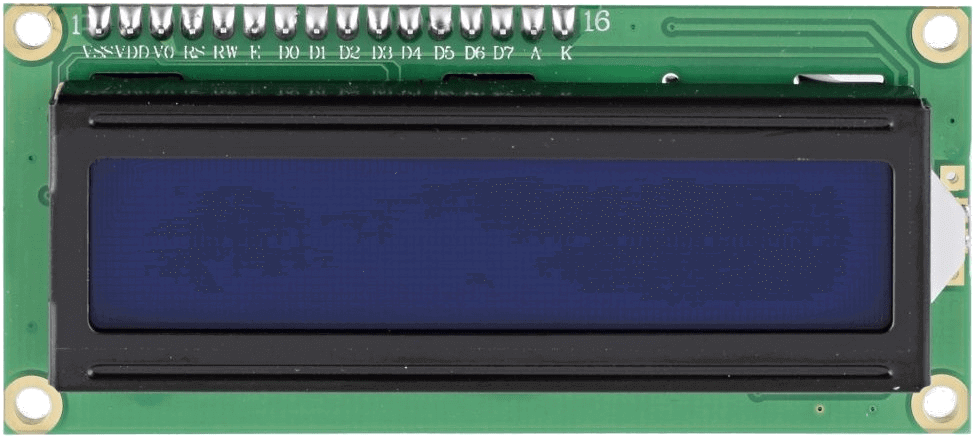
\includegraphics[width=0.9\linewidth]{images/predni-cast-lcd-displeje.png}
  \caption{Přední část displeje.}
  \label{fig:predni-cast-lcd-displeje}
\end{subfigure}%
\begin{subfigure}{.5\textwidth}
  \centering
  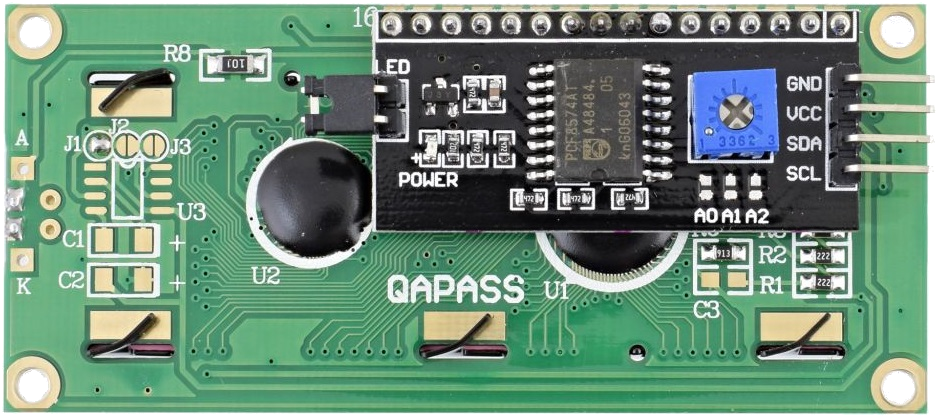
\includegraphics[width=0.9\linewidth]{images/zadni-cast-lcd-displeje-s-expanderem-pcf8574.png}
  \caption{Zadní část displeje s I$^2$C expandérem PCF8574.}
  \label{fig:zadni-cast-lcd-displeje-s-expanderem-pcf857}
\end{subfigure}
\caption[LCD displej pro zobrazování teplot ze zásobníku otopné vody.]{LCD displej pro zobrazování teplot ze zásobníku otopné vody \cite{lcd-displej}.}
\label{fig:lcd-displej}
\end{figure}

\subsubsection{Realizovaná DPS ochran a signalizace u krbů}
Celkové schéma zapojení je v příloze \ref{app:schemata-ostatni}.

\begin{figure}[H]
    \centering
    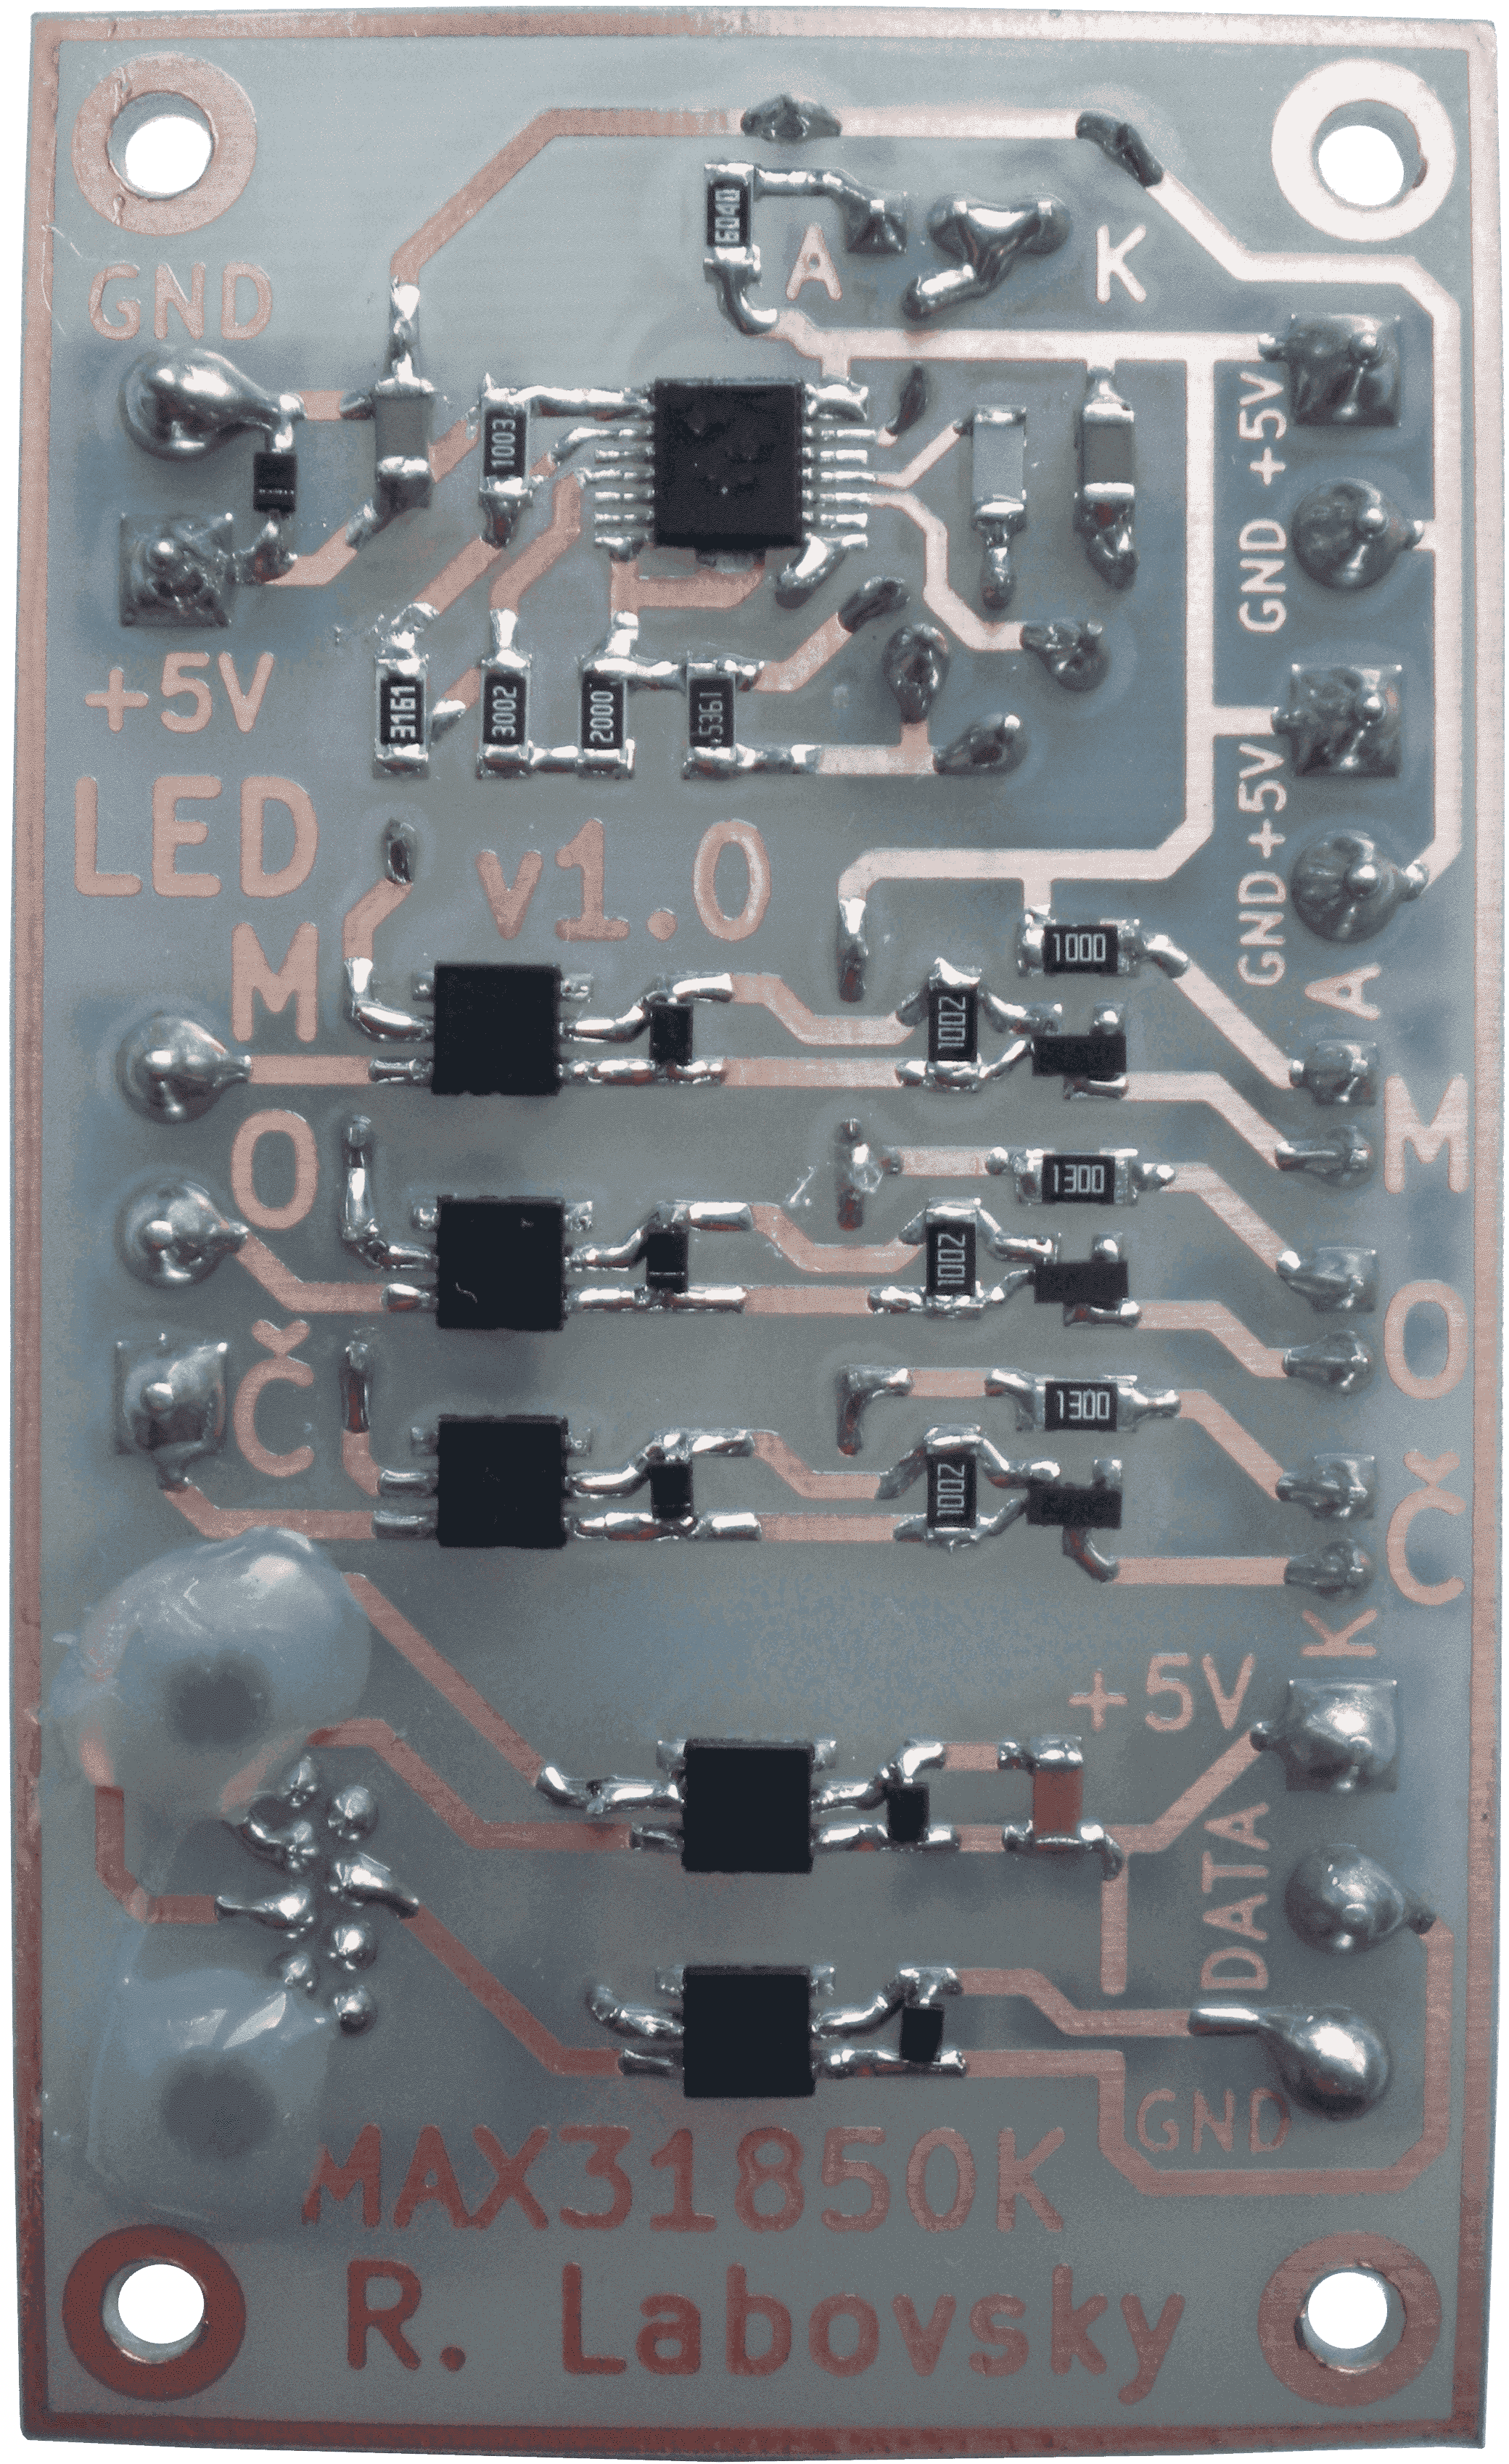
\includegraphics[width=\textwidth]{images/dps-led-ochrany-u-krbu-spodek.png}
    \caption{Spodní část DPS.}
    \label{fig:dps-led-ochrany-u-krbu-spodek}
\end{figure}

\begin{figure}[H]
    \centering
    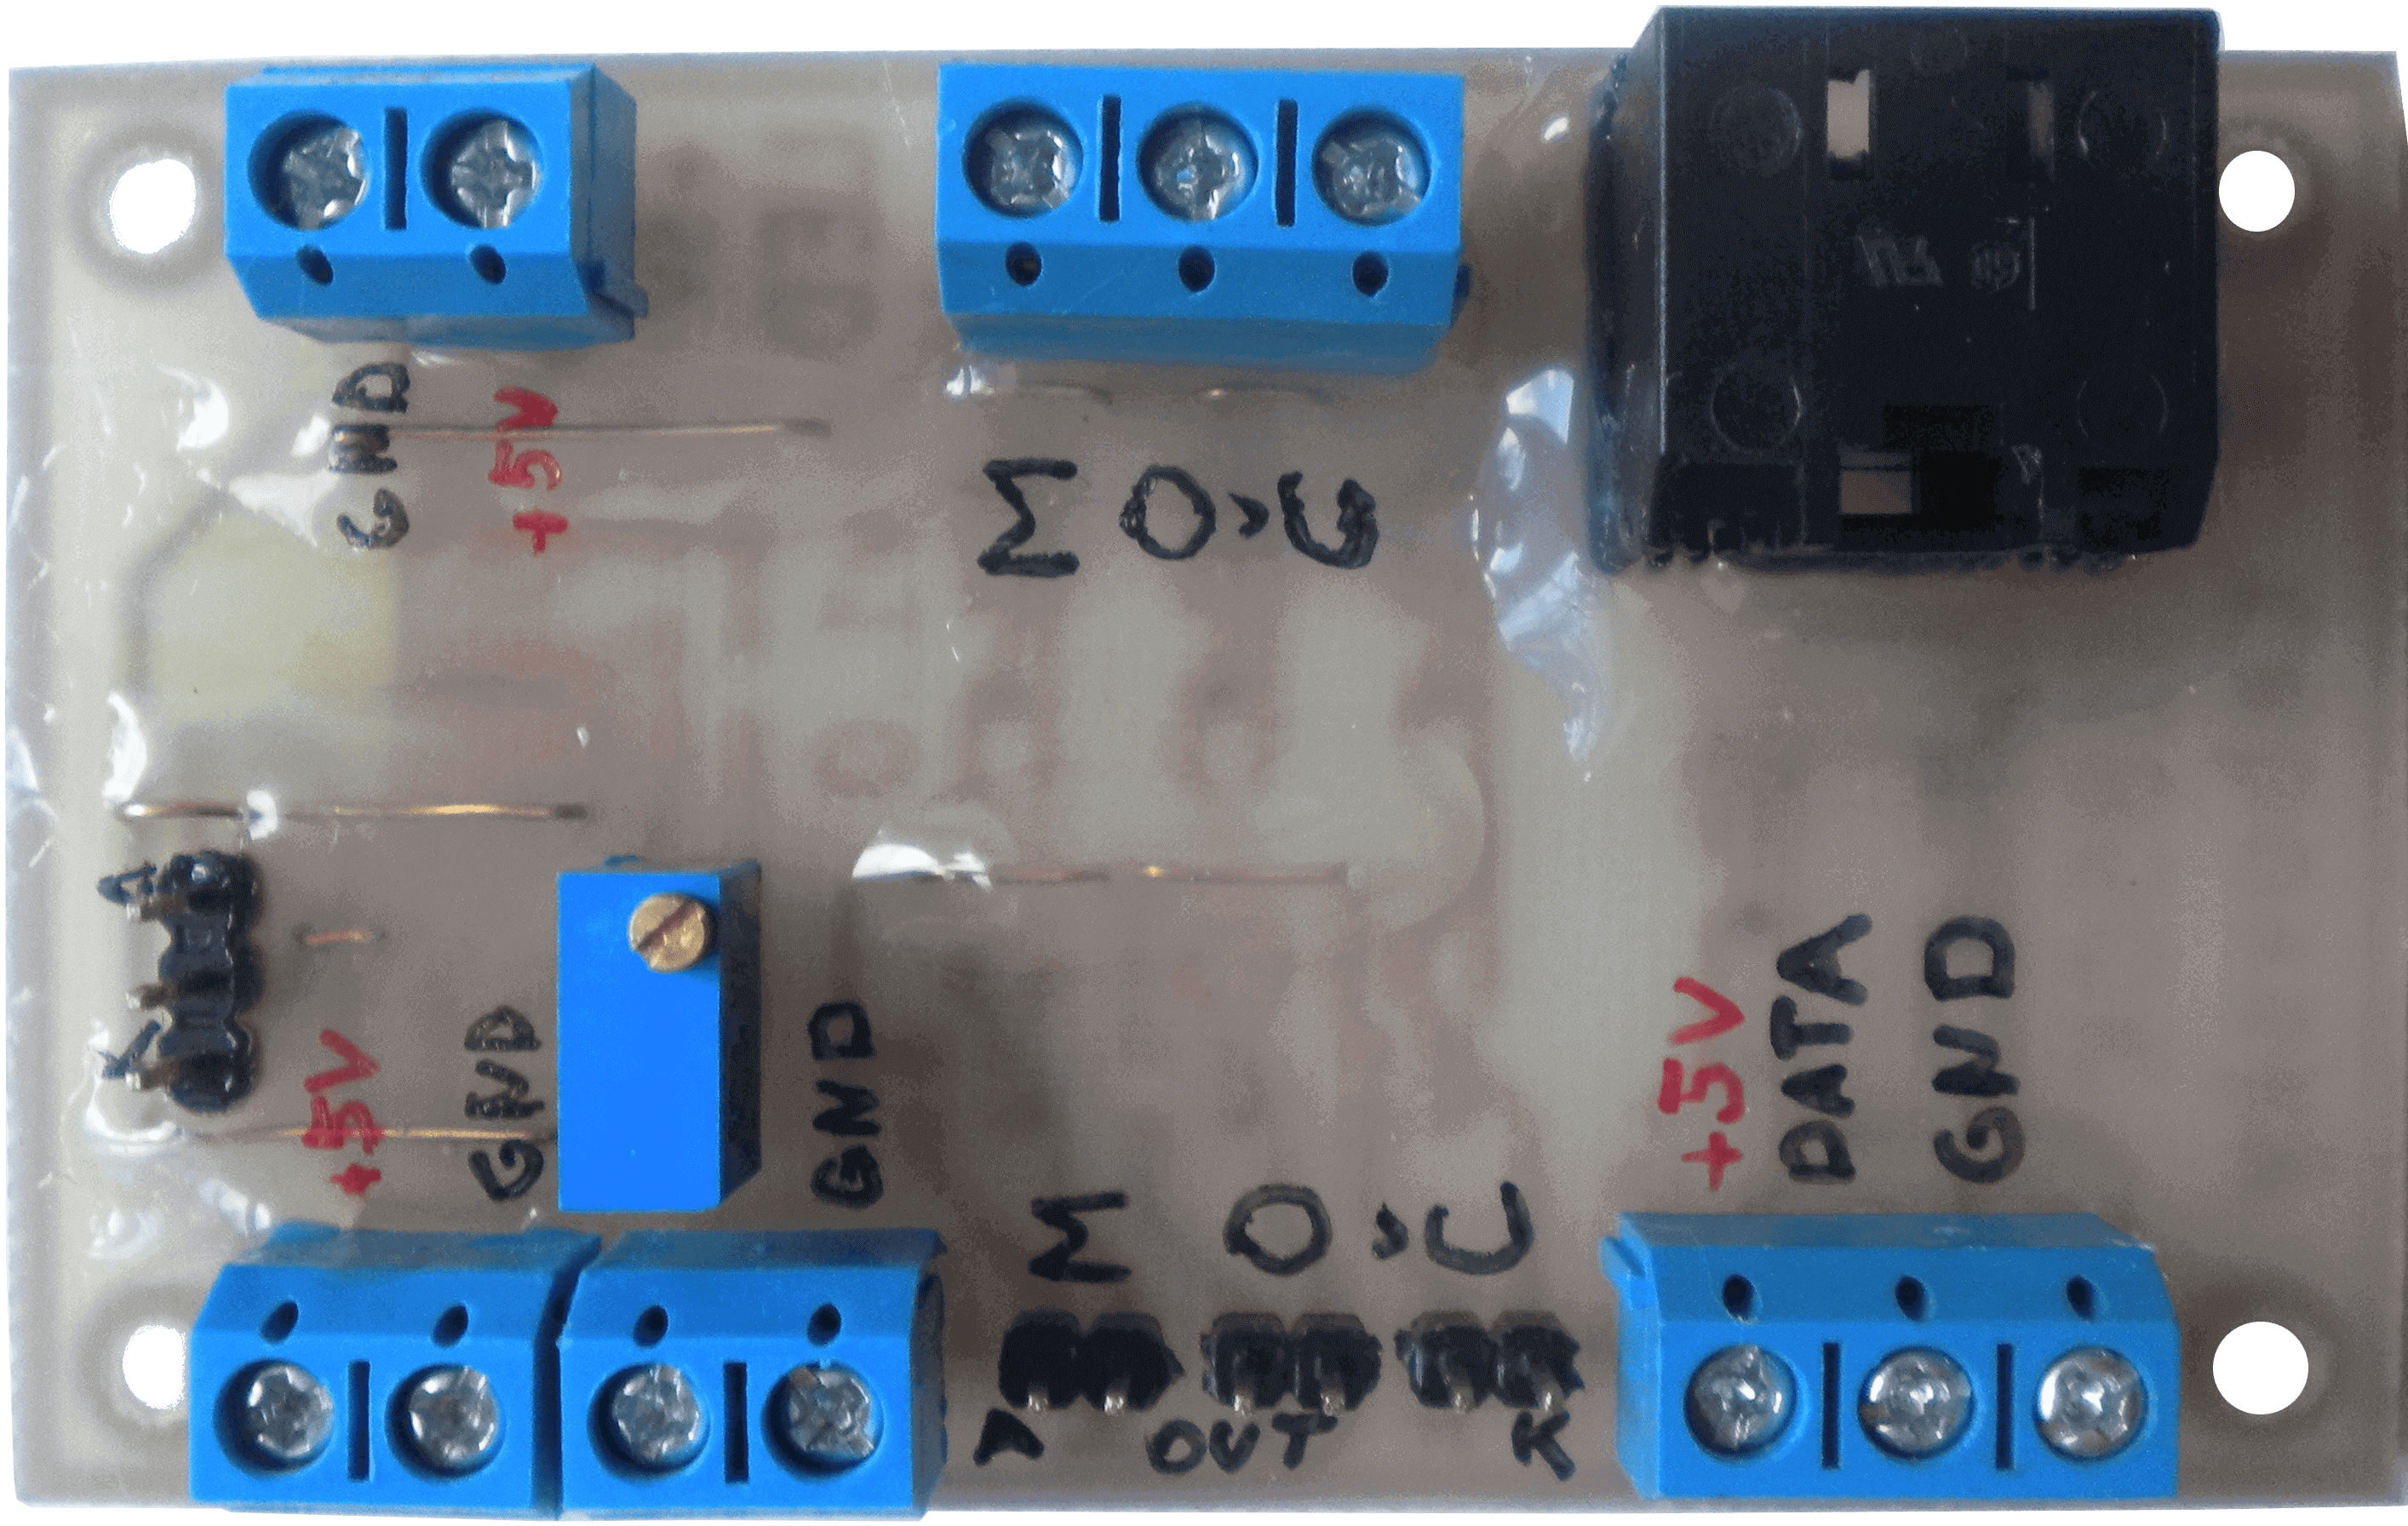
\includegraphics[width=\textwidth]{images/dps-led-ochrany-u-krbu-vrsek.png}
    \caption{Horní část DPS.}
    \label{fig:dps-led-ochrany-u-krbu-vrsek}
\end{figure}

\begin{figure}[H]
    \centering
    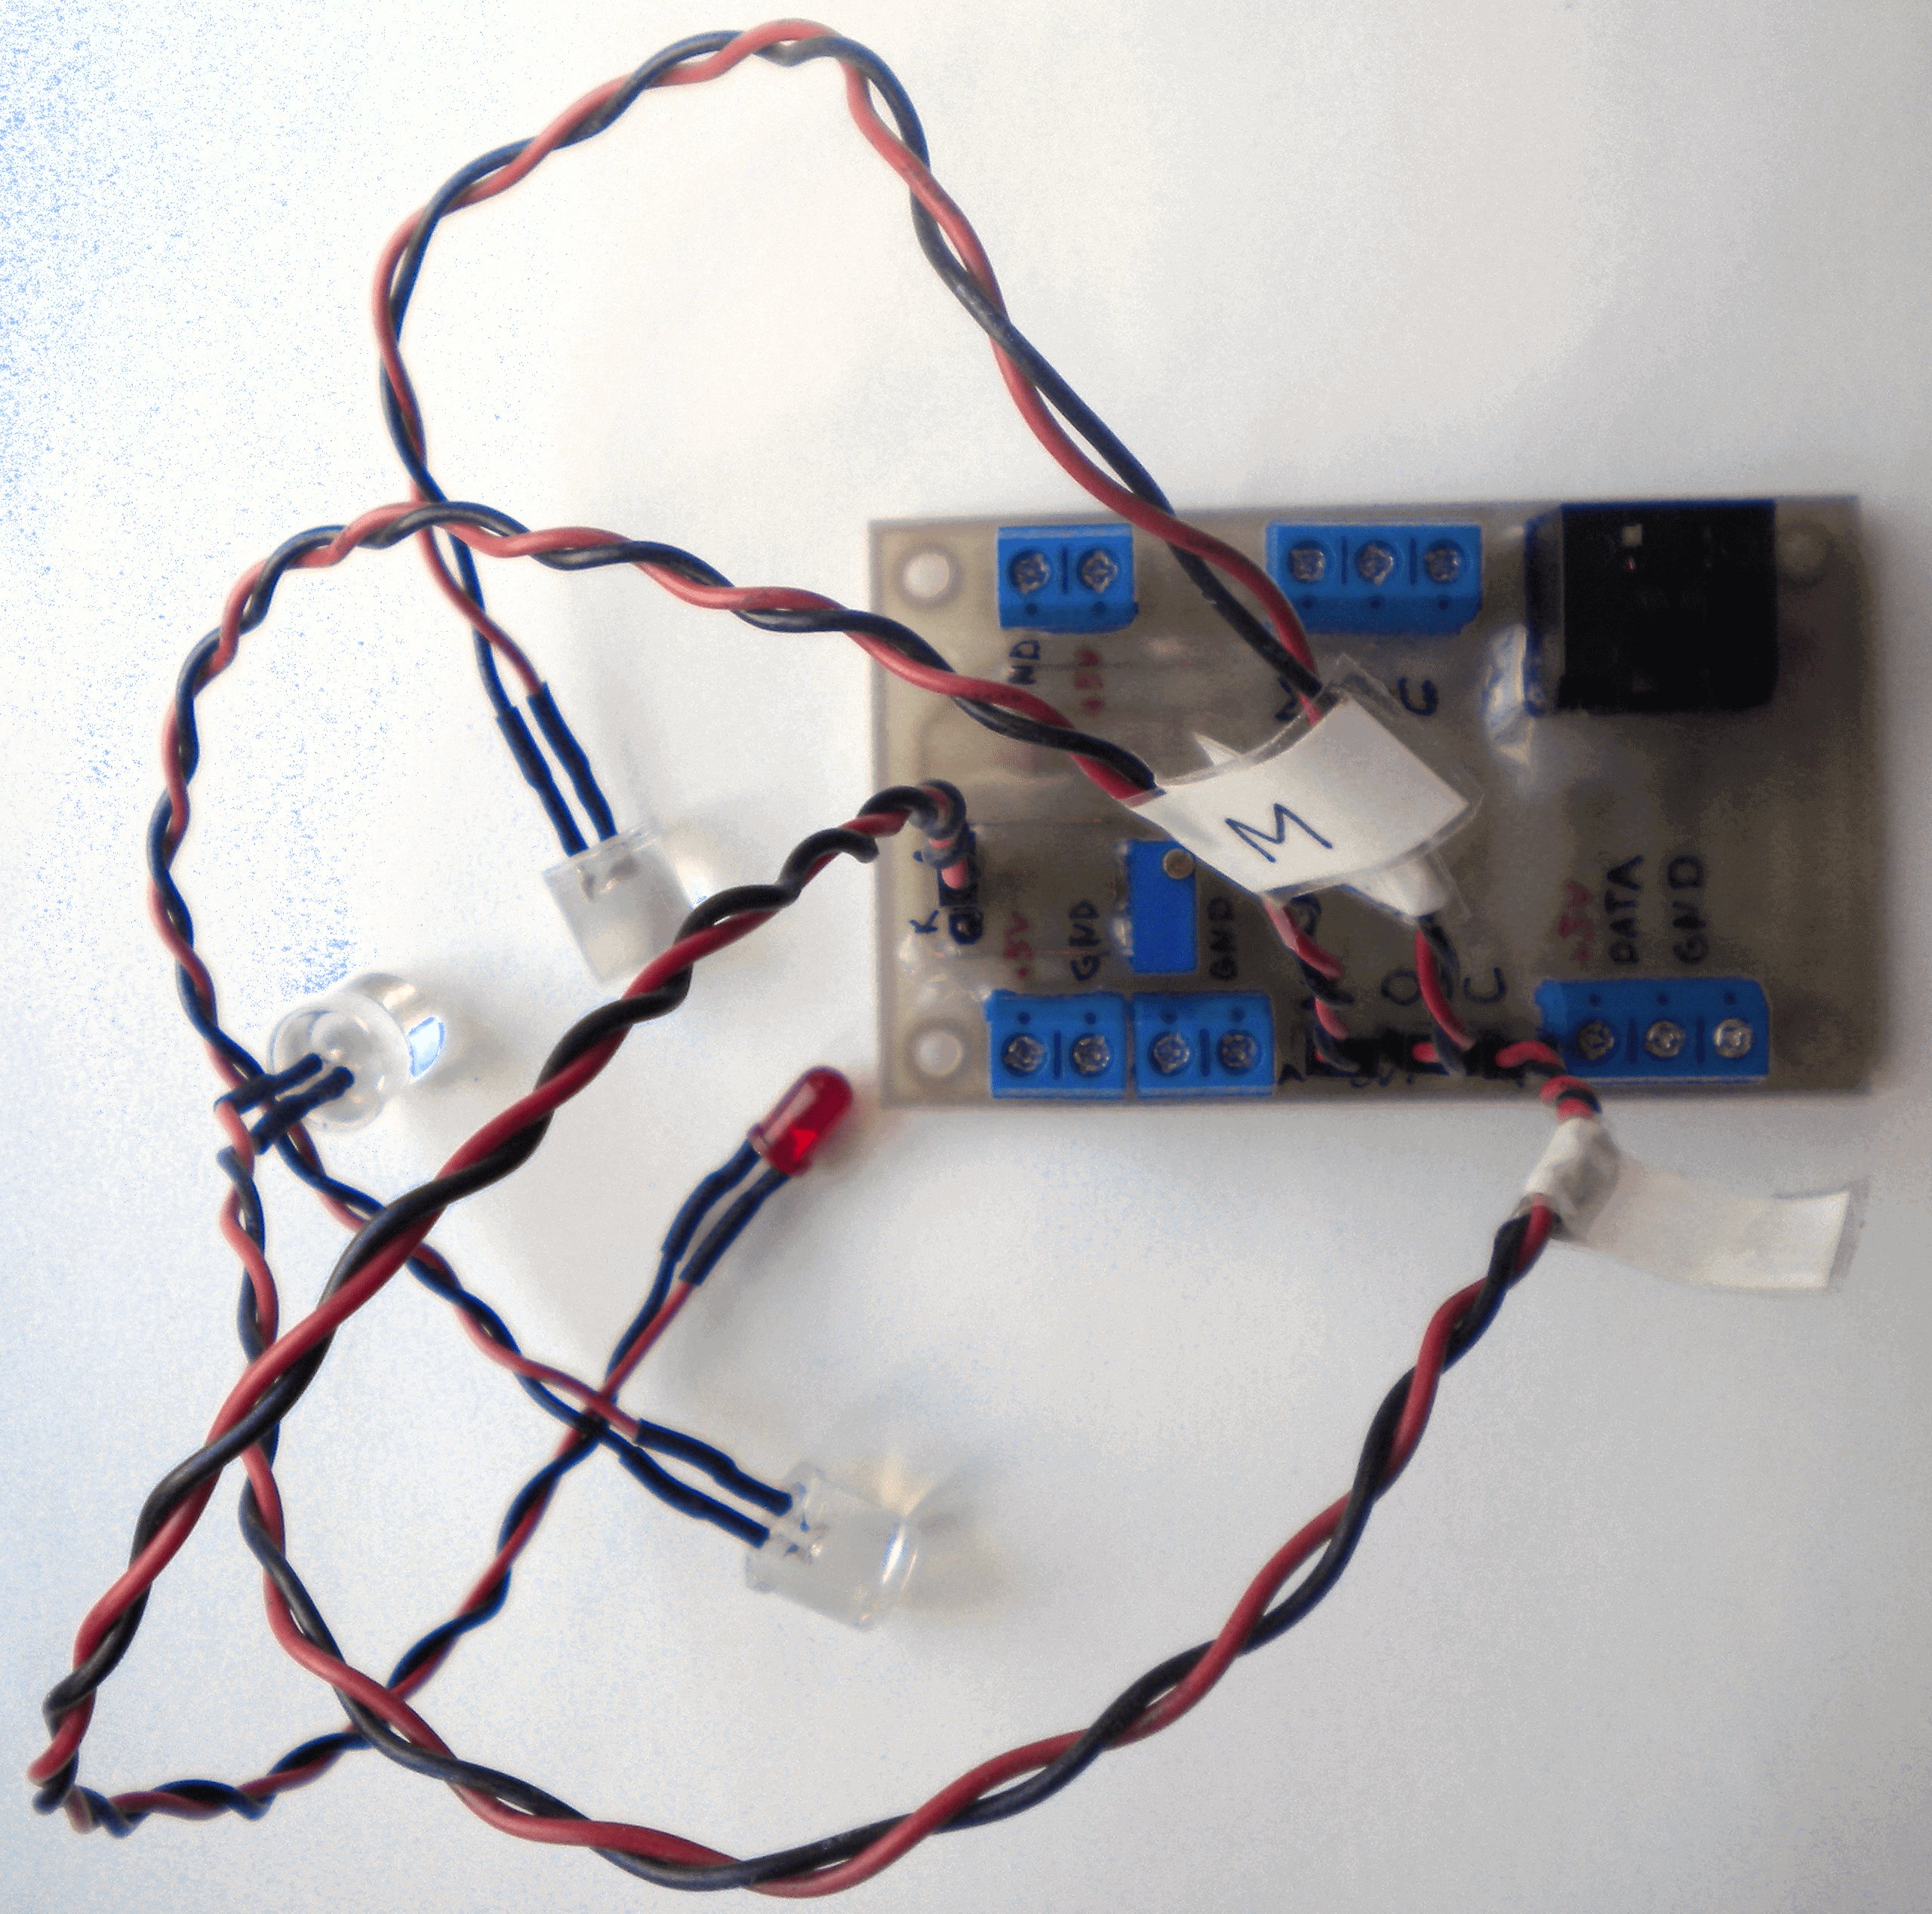
\includegraphics[width=0.95\textwidth]{images/dps-led-ochrany-u-krbu-kabely.png}
    \caption{DPS včetně signalizačních LED.}
    \label{fig:dps-led-ochrany-u-krbu-kabely}
\end{figure}

\subsubsection{Instalační krabice}
Všechna elektronika je umístěna do ochranné instalační krabice (obrázek \ref{fig:instalacni-krabice-vnitrek-krb}). Do krabice vstupují dva vodiče pro napětí 5 V a zem, tři kabely pro ovládání signalizačních LED, UTP kabel se sběrnicí 1-Wire pro teplotní senzor (termočlánek) a I$^2$C sběrnicí. Na obrázku \ref{fig:zadni-cast-krytu-vika-instalacni-krabice-krb} je zobrazena zadní část víka instalační krabice s uchycením signalizačních LED a LCD displeje. Na obrázku \ref{fig:predni-cast-krytu-vika-instalacni-krabice-krb} je přední část víka instalační krabice. Takto zkompletovaná instalační krabice je osazena u krbu ve sklepě, v přízemí a v patře.

\begin{figure}[H]
    \centering
    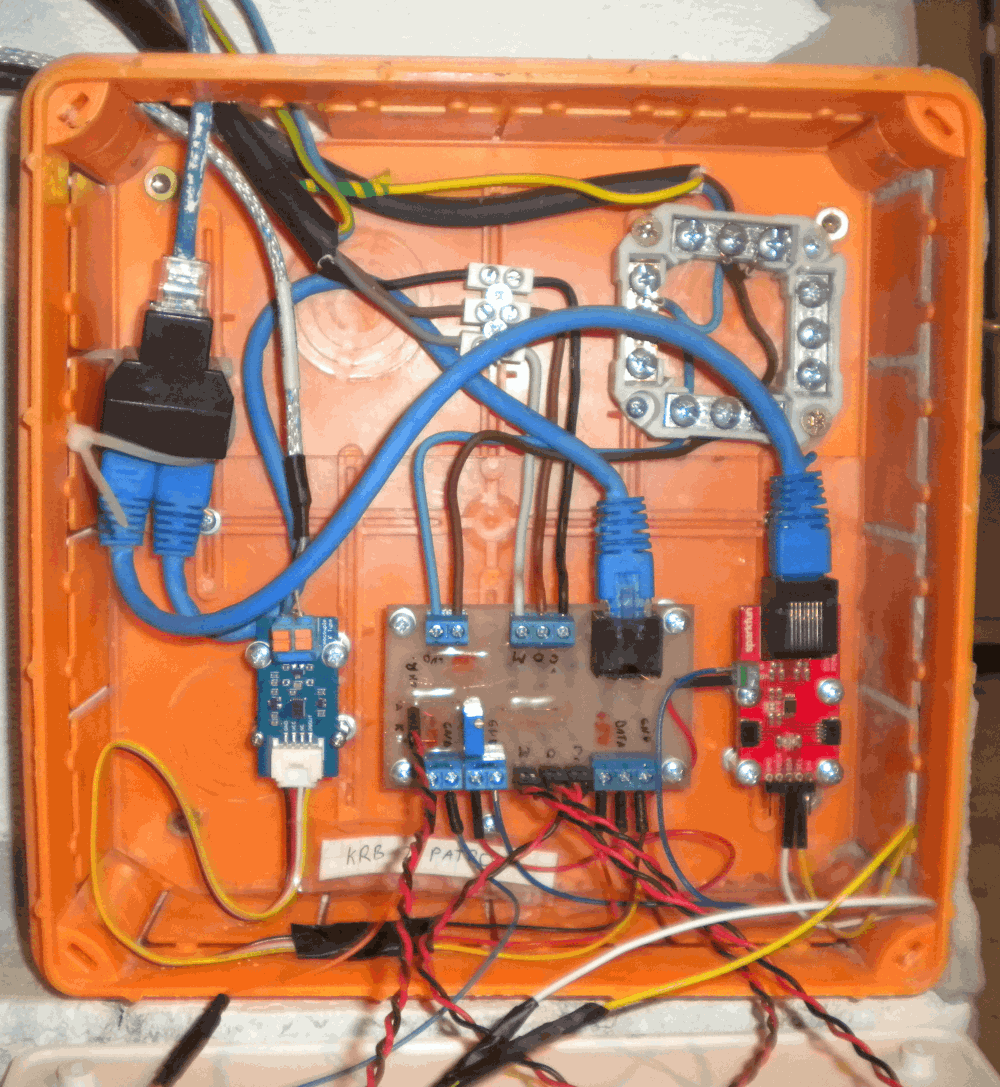
\includegraphics[width=0.6\textwidth]{images/instalacni-krabice-vnitrek-krb.png}
    \caption{Instalační krabice s jednotlivými moduly.}
    \label{fig:instalacni-krabice-vnitrek-krb}
\end{figure}

\begin{figure}[H]
    \centering
    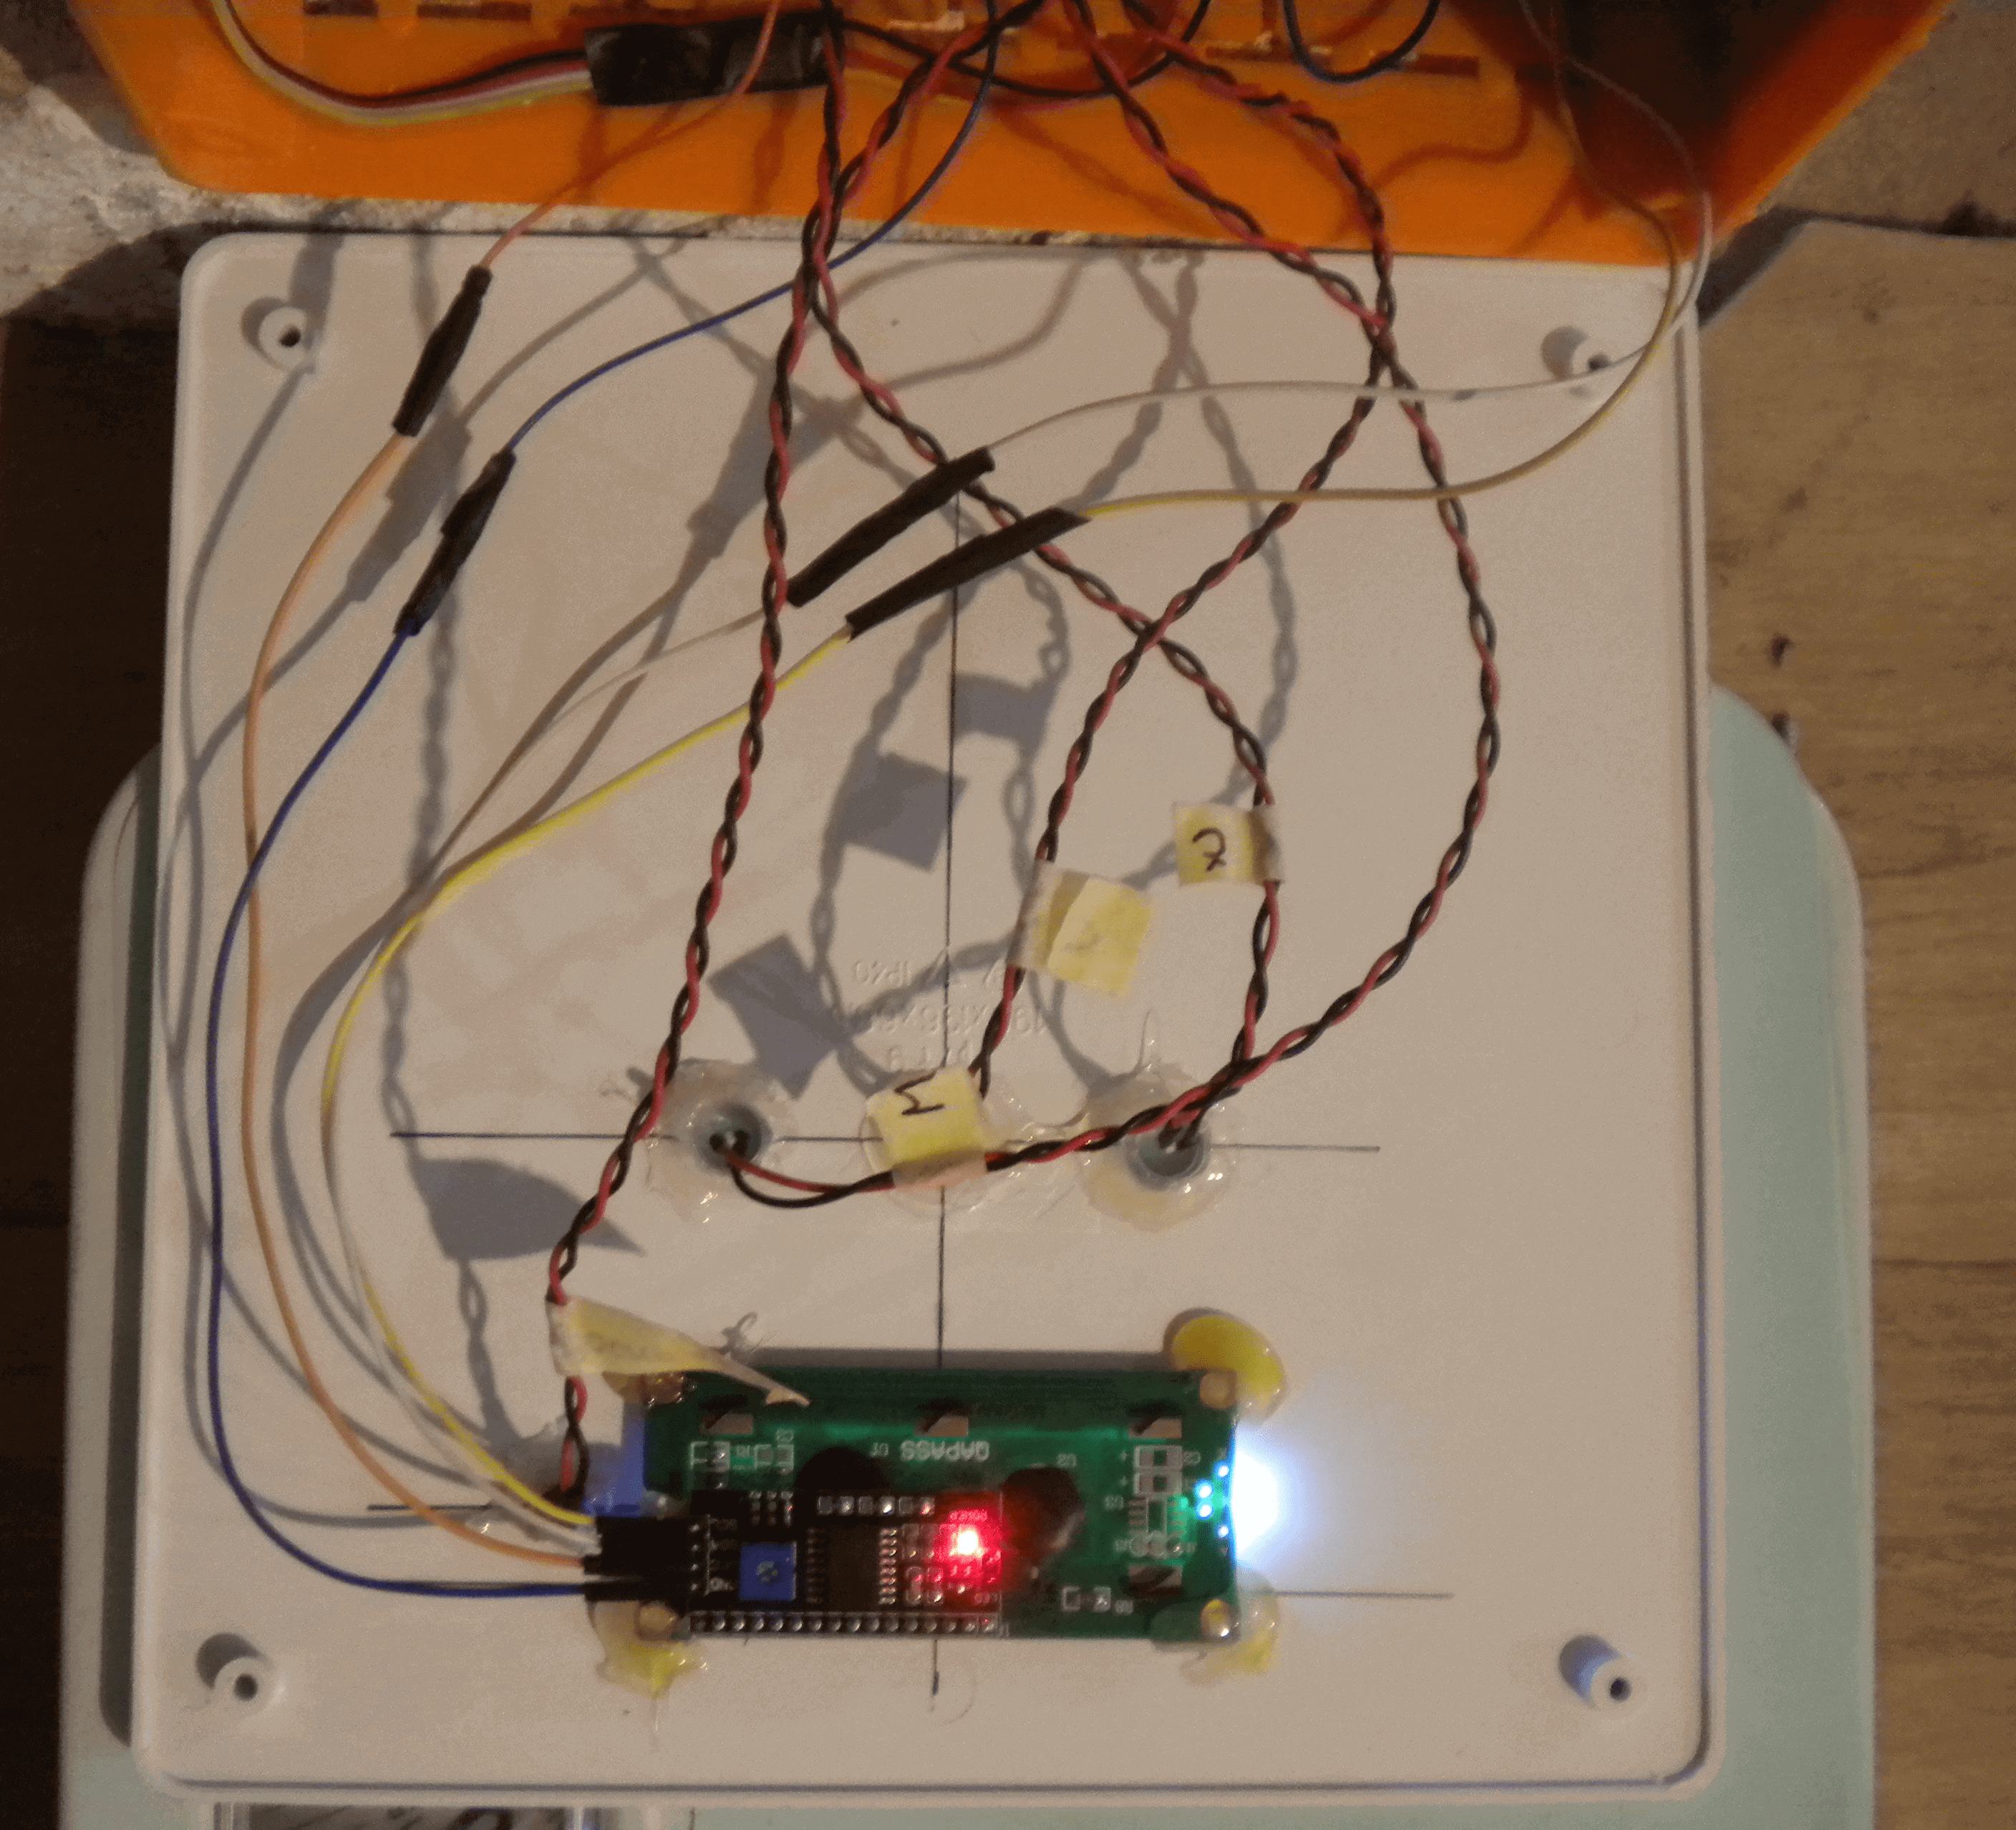
\includegraphics[width=0.6\textwidth]{images/zadni-cast-krytu-vika-instalacni-krabice-krb.png}
    \caption{Zadní část instalační krabice.}
    \label{fig:zadni-cast-krytu-vika-instalacni-krabice-krb}
\end{figure}

\begin{figure}[H]
    \centering
    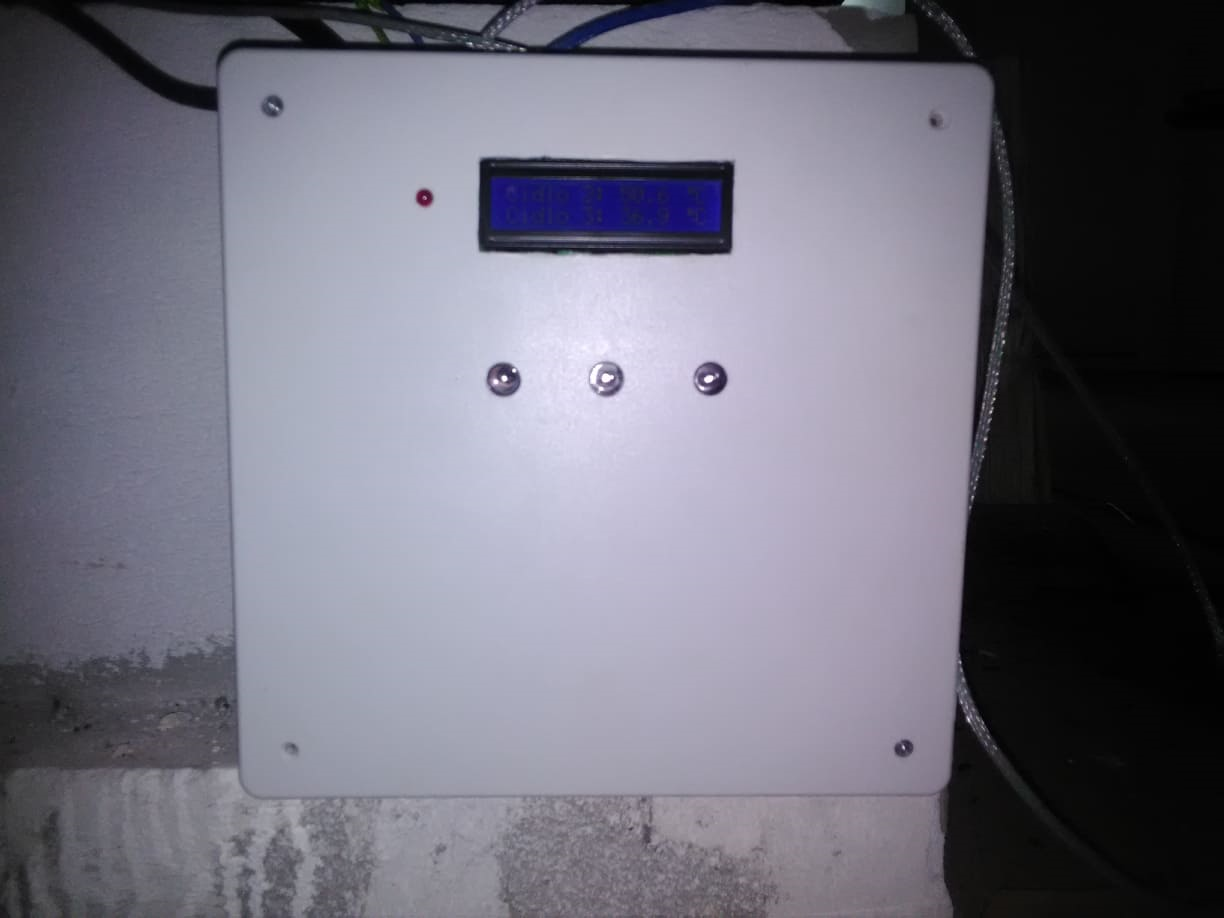
\includegraphics[width=0.6\textwidth]{images/predni-cast-krytu-vika-instalacni-krabice-krb.png}
    \caption[Víko instalační krabice.]{Víko instalační krabice. Osazený LCD displej, signalizačních LED (zleva modrá, oranžová a červená) a LED pro aktivování elektronické pojistky (červená LED vlevo od displeje).}
    \label{fig:predni-cast-krytu-vika-instalacni-krabice-krb}
\end{figure}

\section{Zónový regulátor}
\begin{figure}[H]
   \centering
    \def\svgwidth{0.5\columnwidth}
   \input{images/svg/otopna-soustava/vyrez-zonovy-regulator.pdf_tex}
    \caption[Výřez pro umístění zónového regulátoru v rozdělovači podlahového topení.]{Výřez z obrázku \ref{fig:otopna-soustava-a-elektronika-rez-domu} – umístění zónového regulátoru v rozdělovači podlahového topení.}
    \label{fig:vyrez-zonovy-regulator}
\end{figure}
Na obrázku \ref{fig:vyrez-zonovy-regulator} je výřez části z celkového nákresu (obrázek \ref{fig:otopna-soustava-a-elektronika-rez-domu}) systému znázorňující umístění zónového regulátoru. Zónový regulátor se skládá z modulu PCA9615 (viz část  \ref{sec:i2c-sbernice} (I$^2$C sběrnice)) pro realizaci I$^2$C sběrnice pomocí diferenciálních párů. Samotná sběrnice je realizovaná pomocí UTP kabelu kategorie 5e. Na tento modul je následně napojen obvod PCA9685 \cite{pca9685} od firmy NXP Semiconductors. Výstupy z PCA9685 ovládají jednotlivé termoelektrické pohony (celkově 12 pohonů, každý je řízen samostatně), čímž dochází k regulaci otopné vody do otopných okruhů. Zónové regulátory jsou umístěny v rozdělovači otopných okruhů v přízemí a~patře domu.

\subsubsection{PCA9685}
Obvod PCA9685 umožňuje pomocí I$^2$C sběrnice ovládat 16 výstupů se stejnou individuální hodnotou PWM (se střídou 0 \% až 100 \%), frekvence je programovatelná od 24 Hz do 1\,526 Hz. Každý kanál navíc může dodat 10~mA jako source, případně 25 mA jako sink (což je 160 mA respektive 400~mA celkově).

\subsubsection{DPS pro ovládání termoelektrických pohonů}
Termoelektrické pohony jsou ovládány na základě hodnoty PWM z modulu PCA9685 (viz předchozí bod), každý výstup ovládá jednotlivý pohon. V~praxi se však ukázalo, že nelze dostatečně přesně a v krátké době regulovat posuv pístu daného pohonu pomocí PWM regulace, proto se využívají jen hodnoty PWM 0\% (vypnutý stav) PWM 100 \% (zapnutý stav). Vzhledem k tomu, že termoelektrické pohony jsou na stejnosměrné napětí 24 V, je nutné využít napěťový převodník z 5 V na 24 V. K tomu slouží tranzistor MOSFET (DMN3023L-7 \cite{dmn3023l}). Paralelně k~tranzistoru se nachází přepínač, který slouží v případě poruchy k manuálnímu zapnutí/vypnutí pohonu.  Každý kanál obsahuje indikační zelenou LED pro ovládání. Jak již bylo řečeno pohony jsou napájeny pomocí 24 V, jsou vytvořené dvě napájecí větve s obvodem TPC26600 (popsaný v části \ref{sec:napajeni-1-wire-sbernice}), rozdíl spočívá ve vstupním napájení, které činí 24 V. Jsou tedy rozdílné i~maximální a~minimální povolené meze, které činí max. 24,25 V a min. 10~V. Dále každá větev má nastavený maximální proud 1,5 A (každý pohon má maximální hodnotu proudu při zapnutí 250 mA pro celkově 6 pohonů na větev). Vzhledem k jednoduchosti obvodu TPS26600 a k jeho vlastnostem (především pro automatickou detekci odstranění závady, bez nutnosti restartu zařízení) bylo raději zvoleno zapojení se dvěma větvemi (maximální proud pro TPS26600 činí 2,21 A) než využití jiného integrovaného obvodu pro sloučení do jedné větve. Na obrázku \ref{fig:zonovy-regulator-mosfet-pwm-1-kanal} je zapojení jednoho kanálu pro ovládání termoelektrického pohonu.  Na obrázku \ref{fig:dps-zonovy-regulator-spodni-strana} spodní strana realizované DPS a na obrázku \ref{fig:zonovy-regulator-vrchni-strana} je vrchní strana, včetně osazeného modulu s obvodem PCA9615. Na obrázku \ref{fig:zonovy-regulator-spodni-strana} je spodní část panelu s DPS zónového regulátoru a na obrázku \ref{fig:zonovy-regulator-vrchni-strana} je čelní část panelu. Deska byla vlastnoručně navržena, vyrobena a osazena. Je aplikován ochranný lak. Celkové schéma zapojení je v příloze \ref{app:schemata-ostatni}. Umístění DPS v samotném rozdělovači je v příloze \ref{app:rozdelovac-podlahoveho-vytapeni}.


\begin{figure}[H]
    \centering
    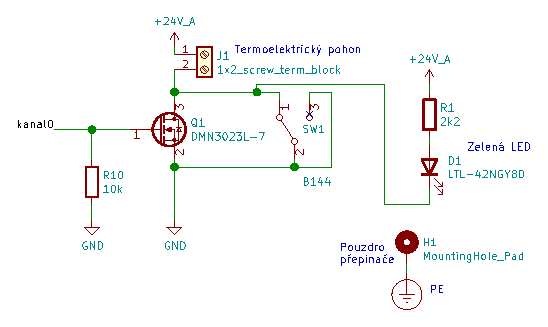
\includegraphics[width=\textwidth]{images/svg/kicad/zonovy-regulator-mosfet-pwm-1-kanal.eps}
    \caption{Zapojení jednoho kanálu pro ovládání termoelektrického pohonu.}
    \label{fig:zonovy-regulator-mosfet-pwm-1-kanal}
\end{figure}

\begin{figure}[H]
    \centering
    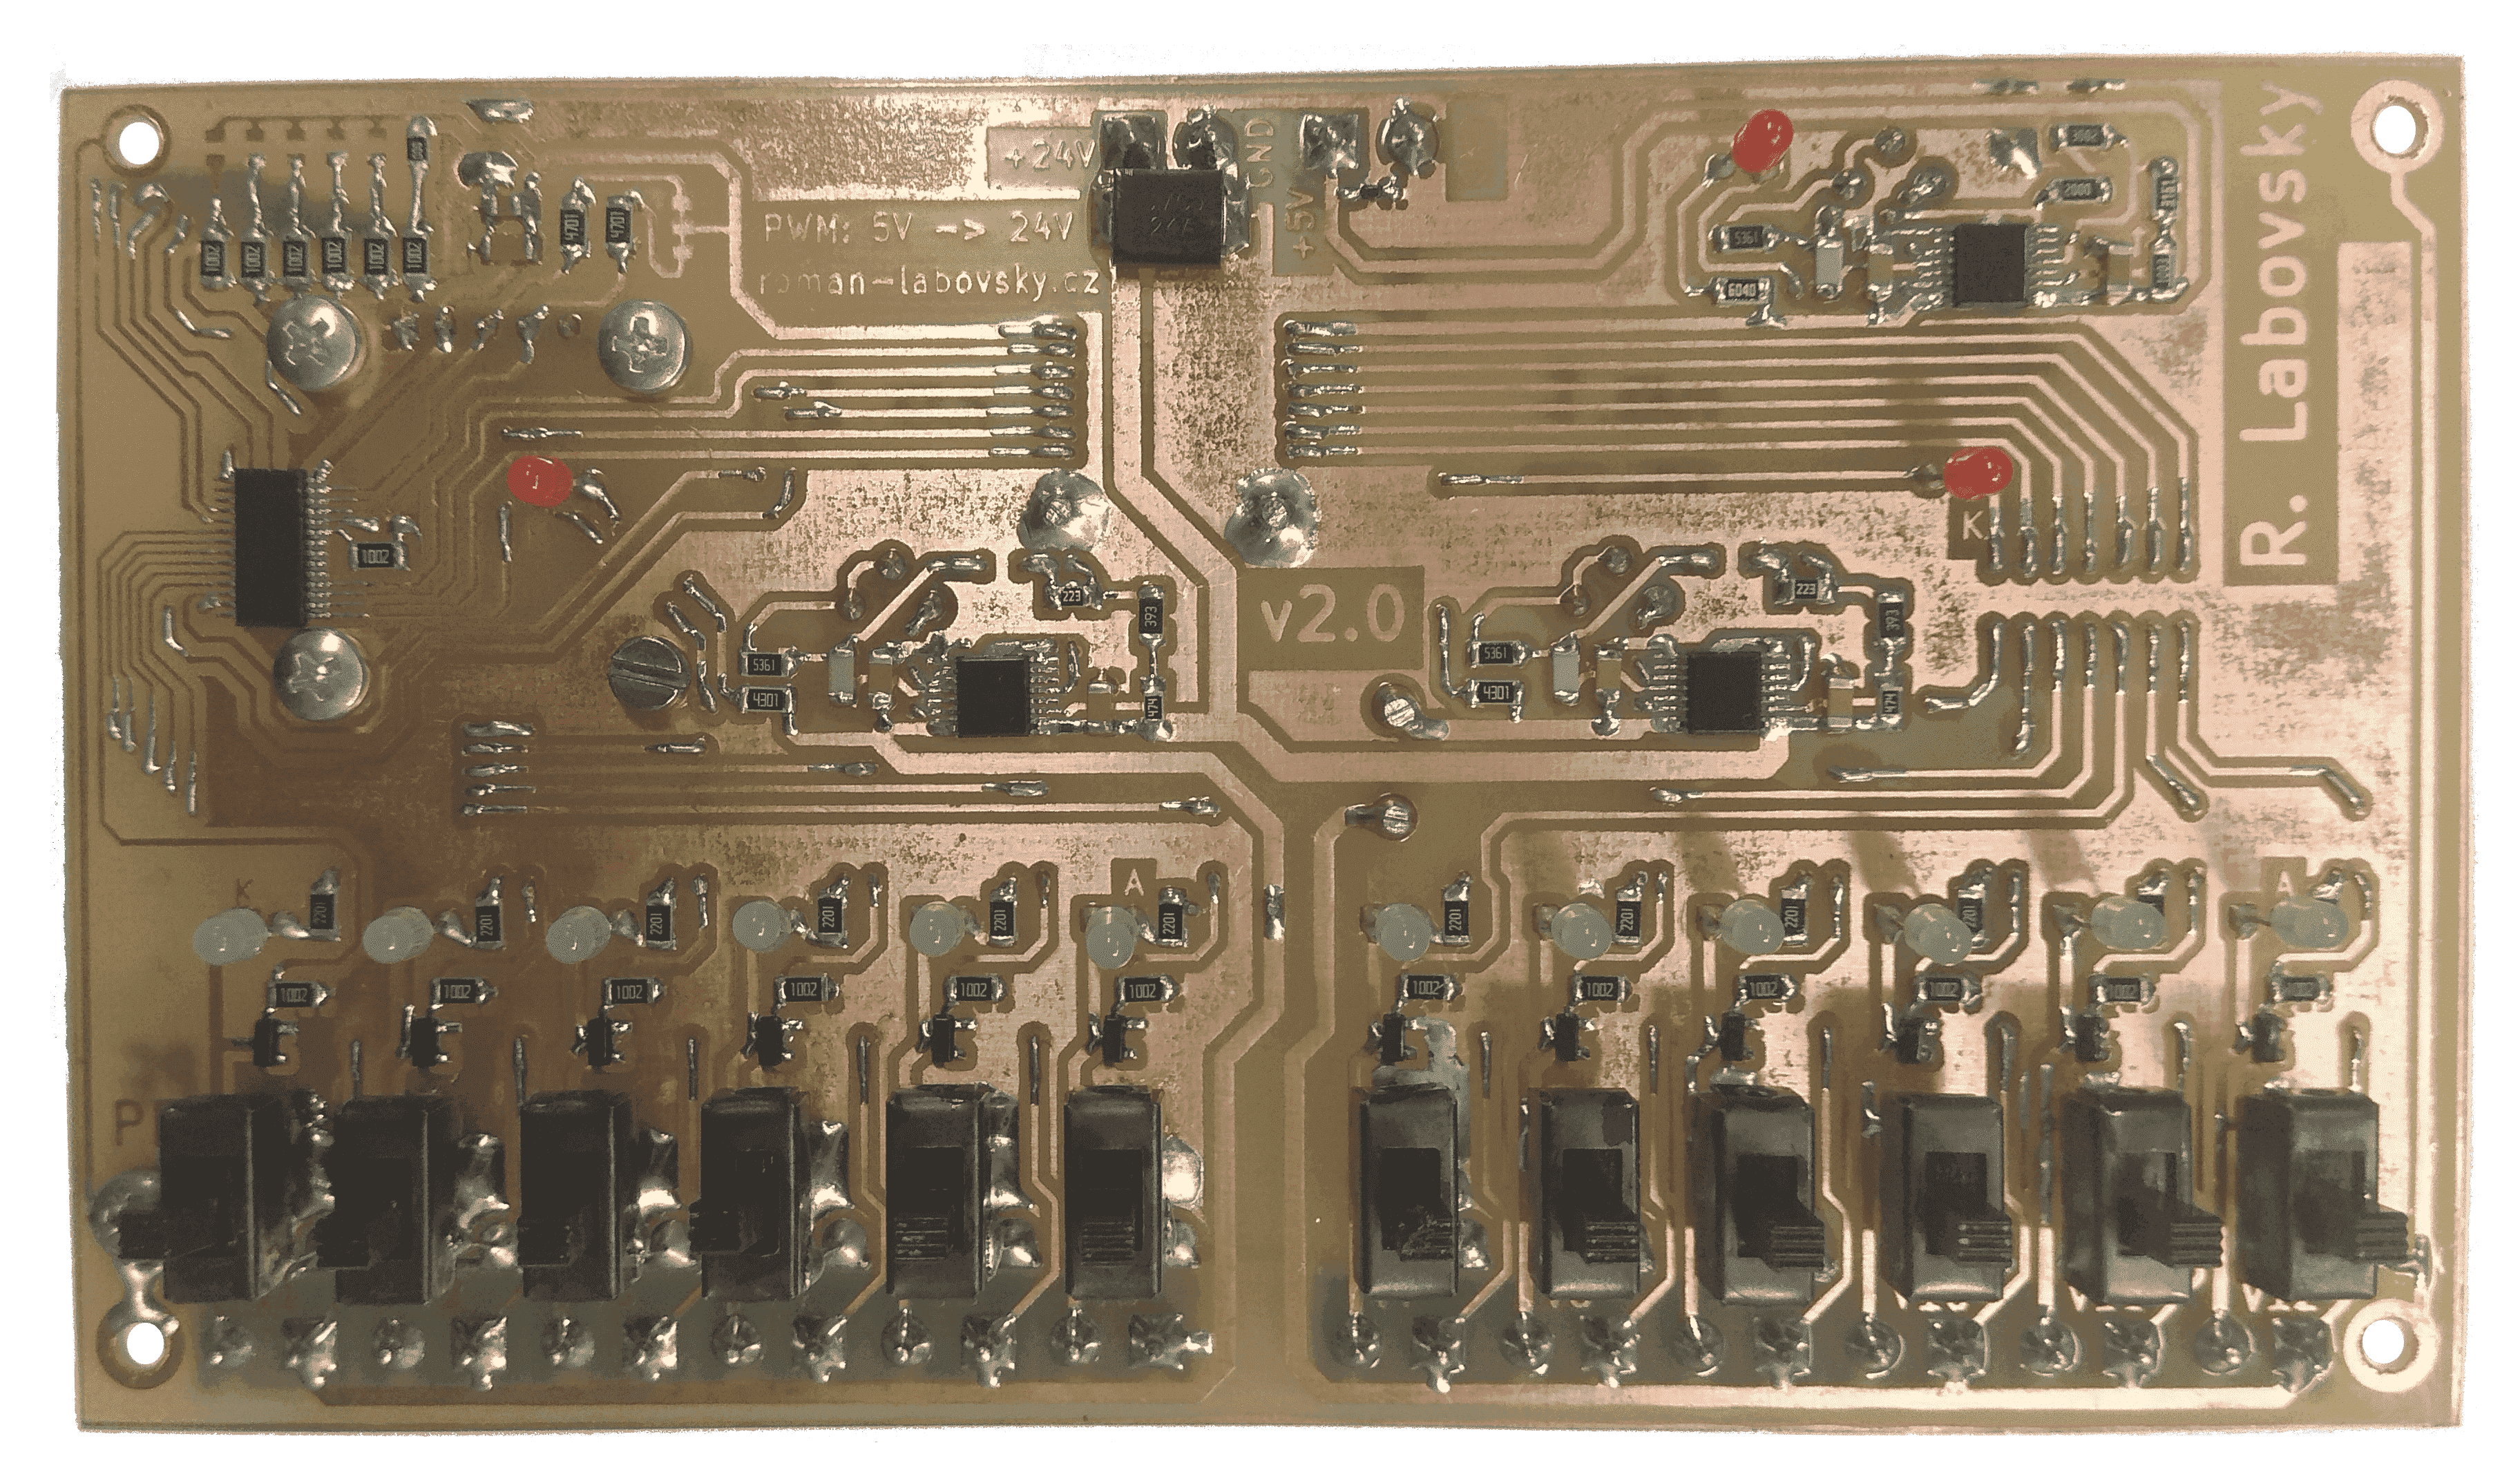
\includegraphics[width=0.99\textwidth]{images/zonovy-regulator/dps-zonovy-regulator-spodni-strana.png}
    \caption{DPS zónového regulátoru, spodní strana.}
    \label{fig:dps-zonovy-regulator-spodni-strana}
\end{figure}

\begin{figure}[H]
    \centering
    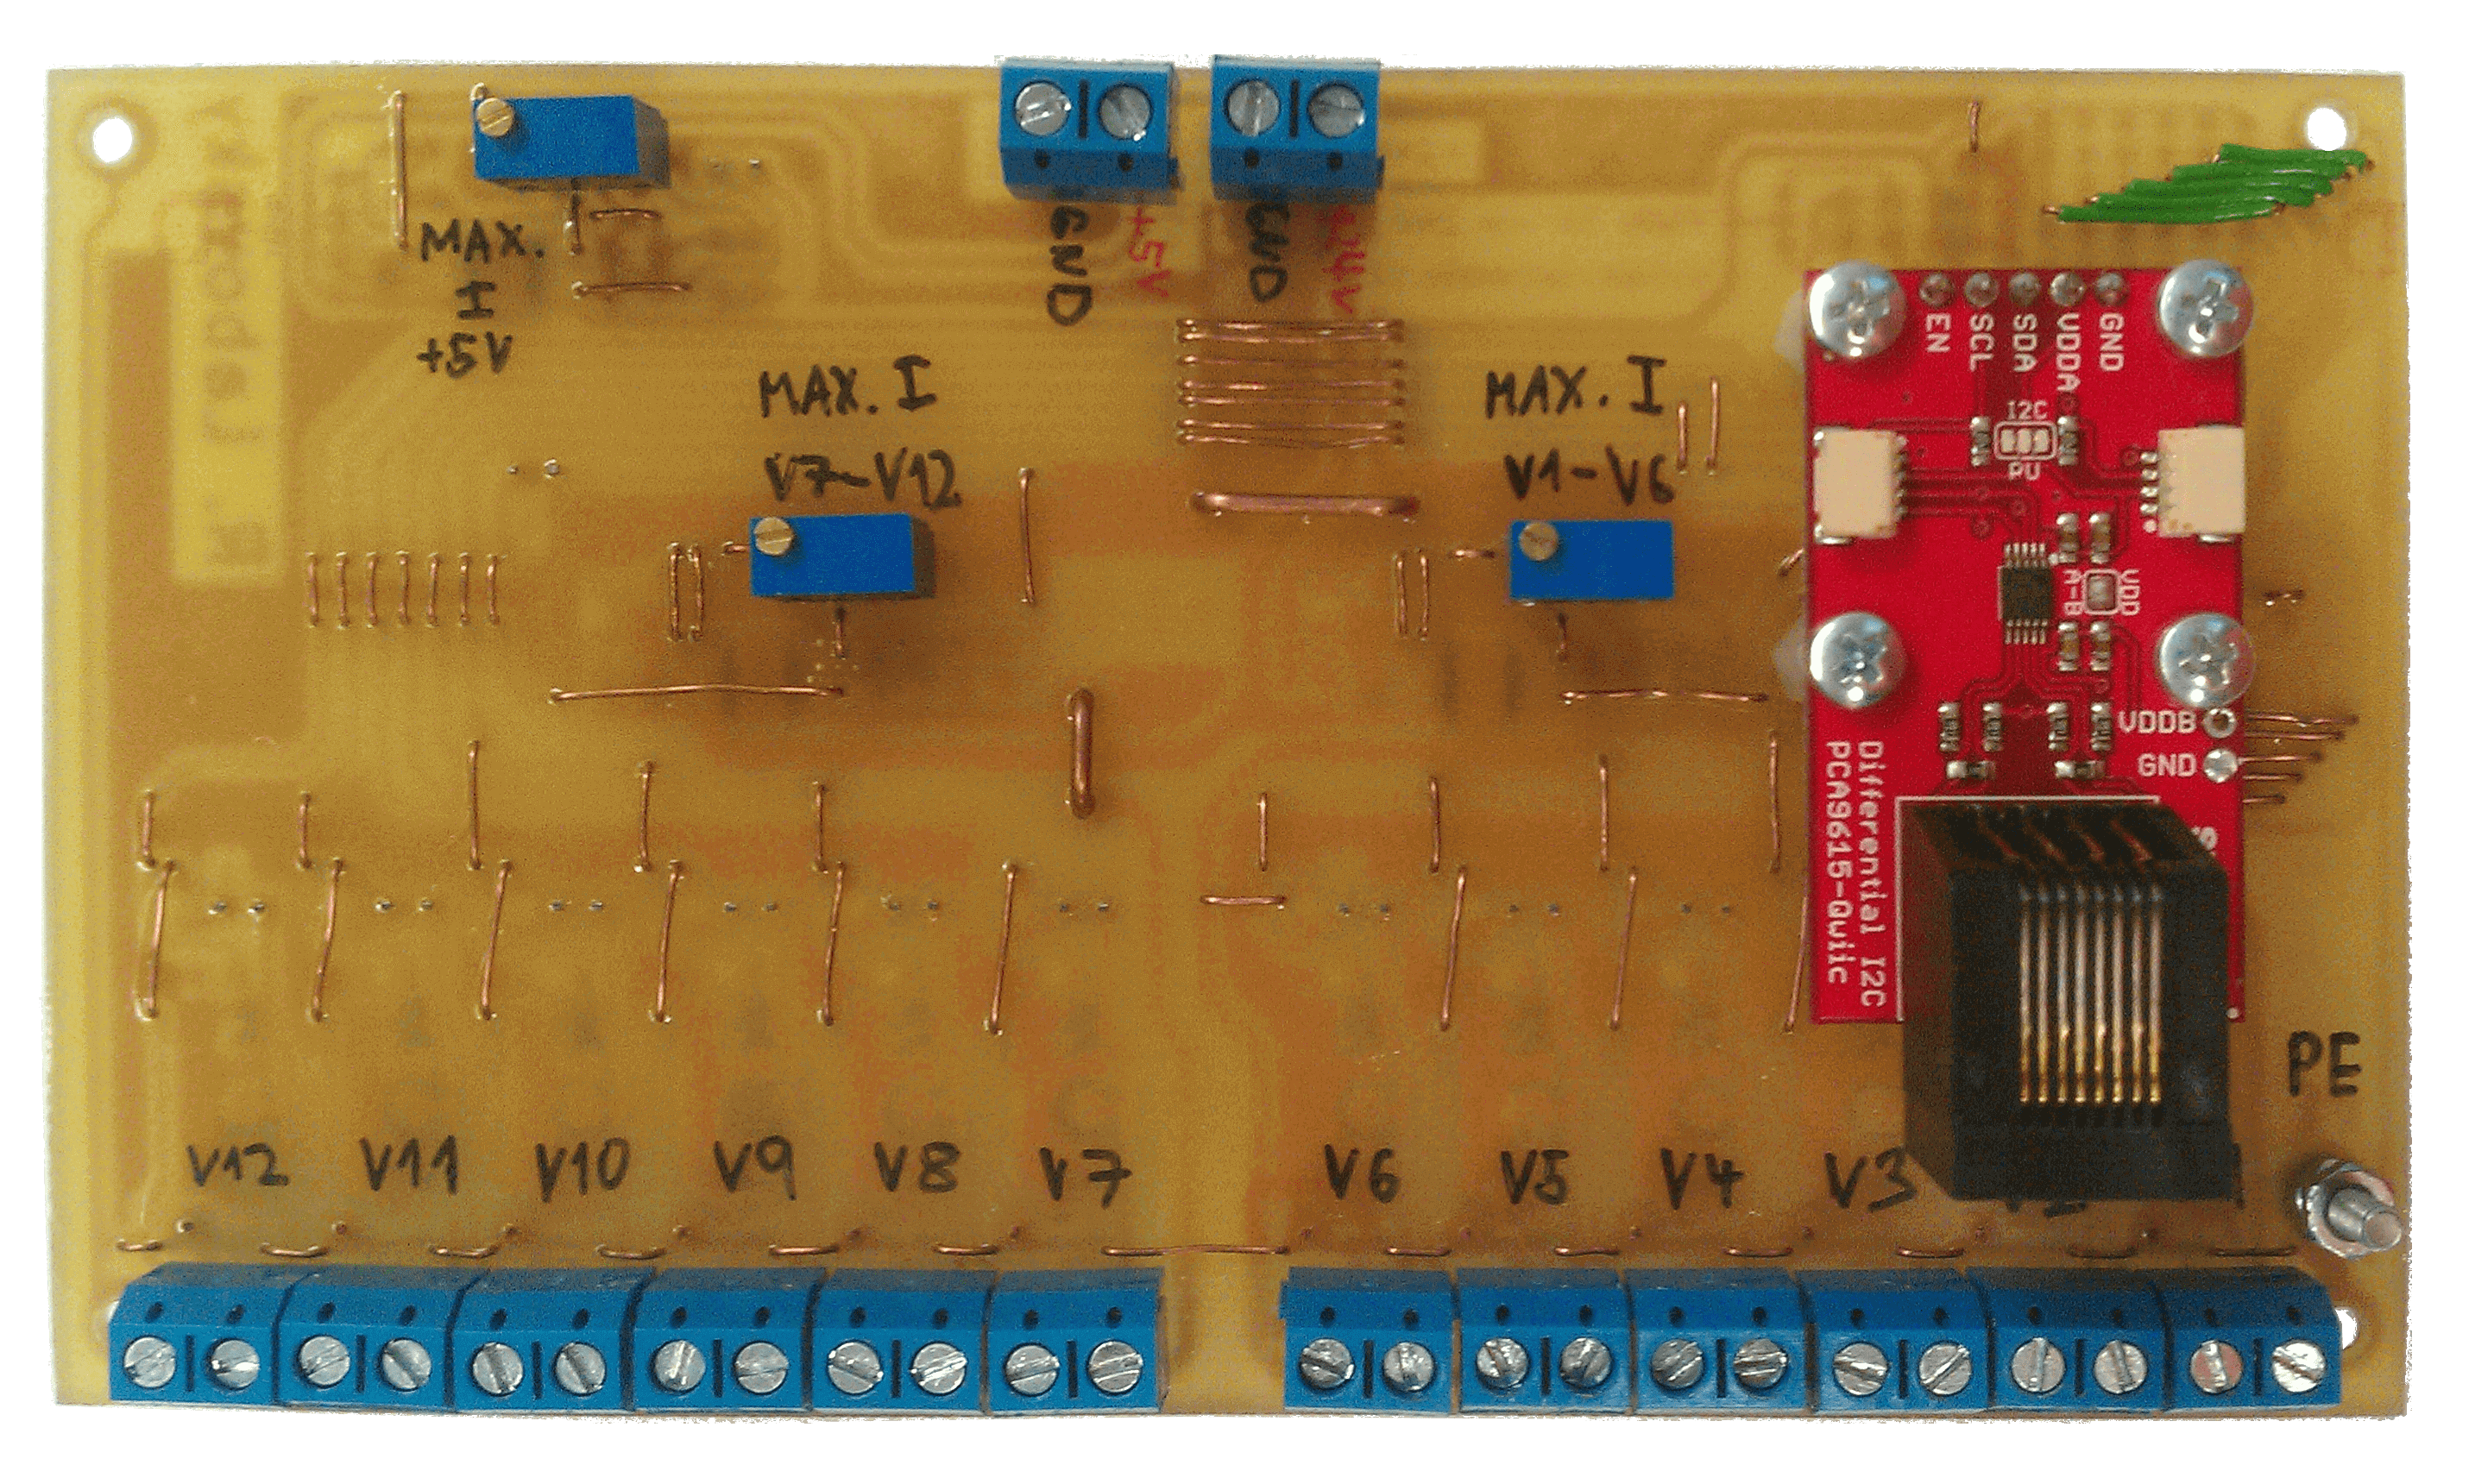
\includegraphics[width=0.99\textwidth]{images/zonovy-regulator/dps-zonovy-regulator-vrchni-strana.png}
    \caption{DPS zónového regulátoru, vrchní strana.}
    \label{fig:dps-zonovy-regulator-vrchni-strana}
\end{figure}


%\begin{figure}[H]
%    \centering
%    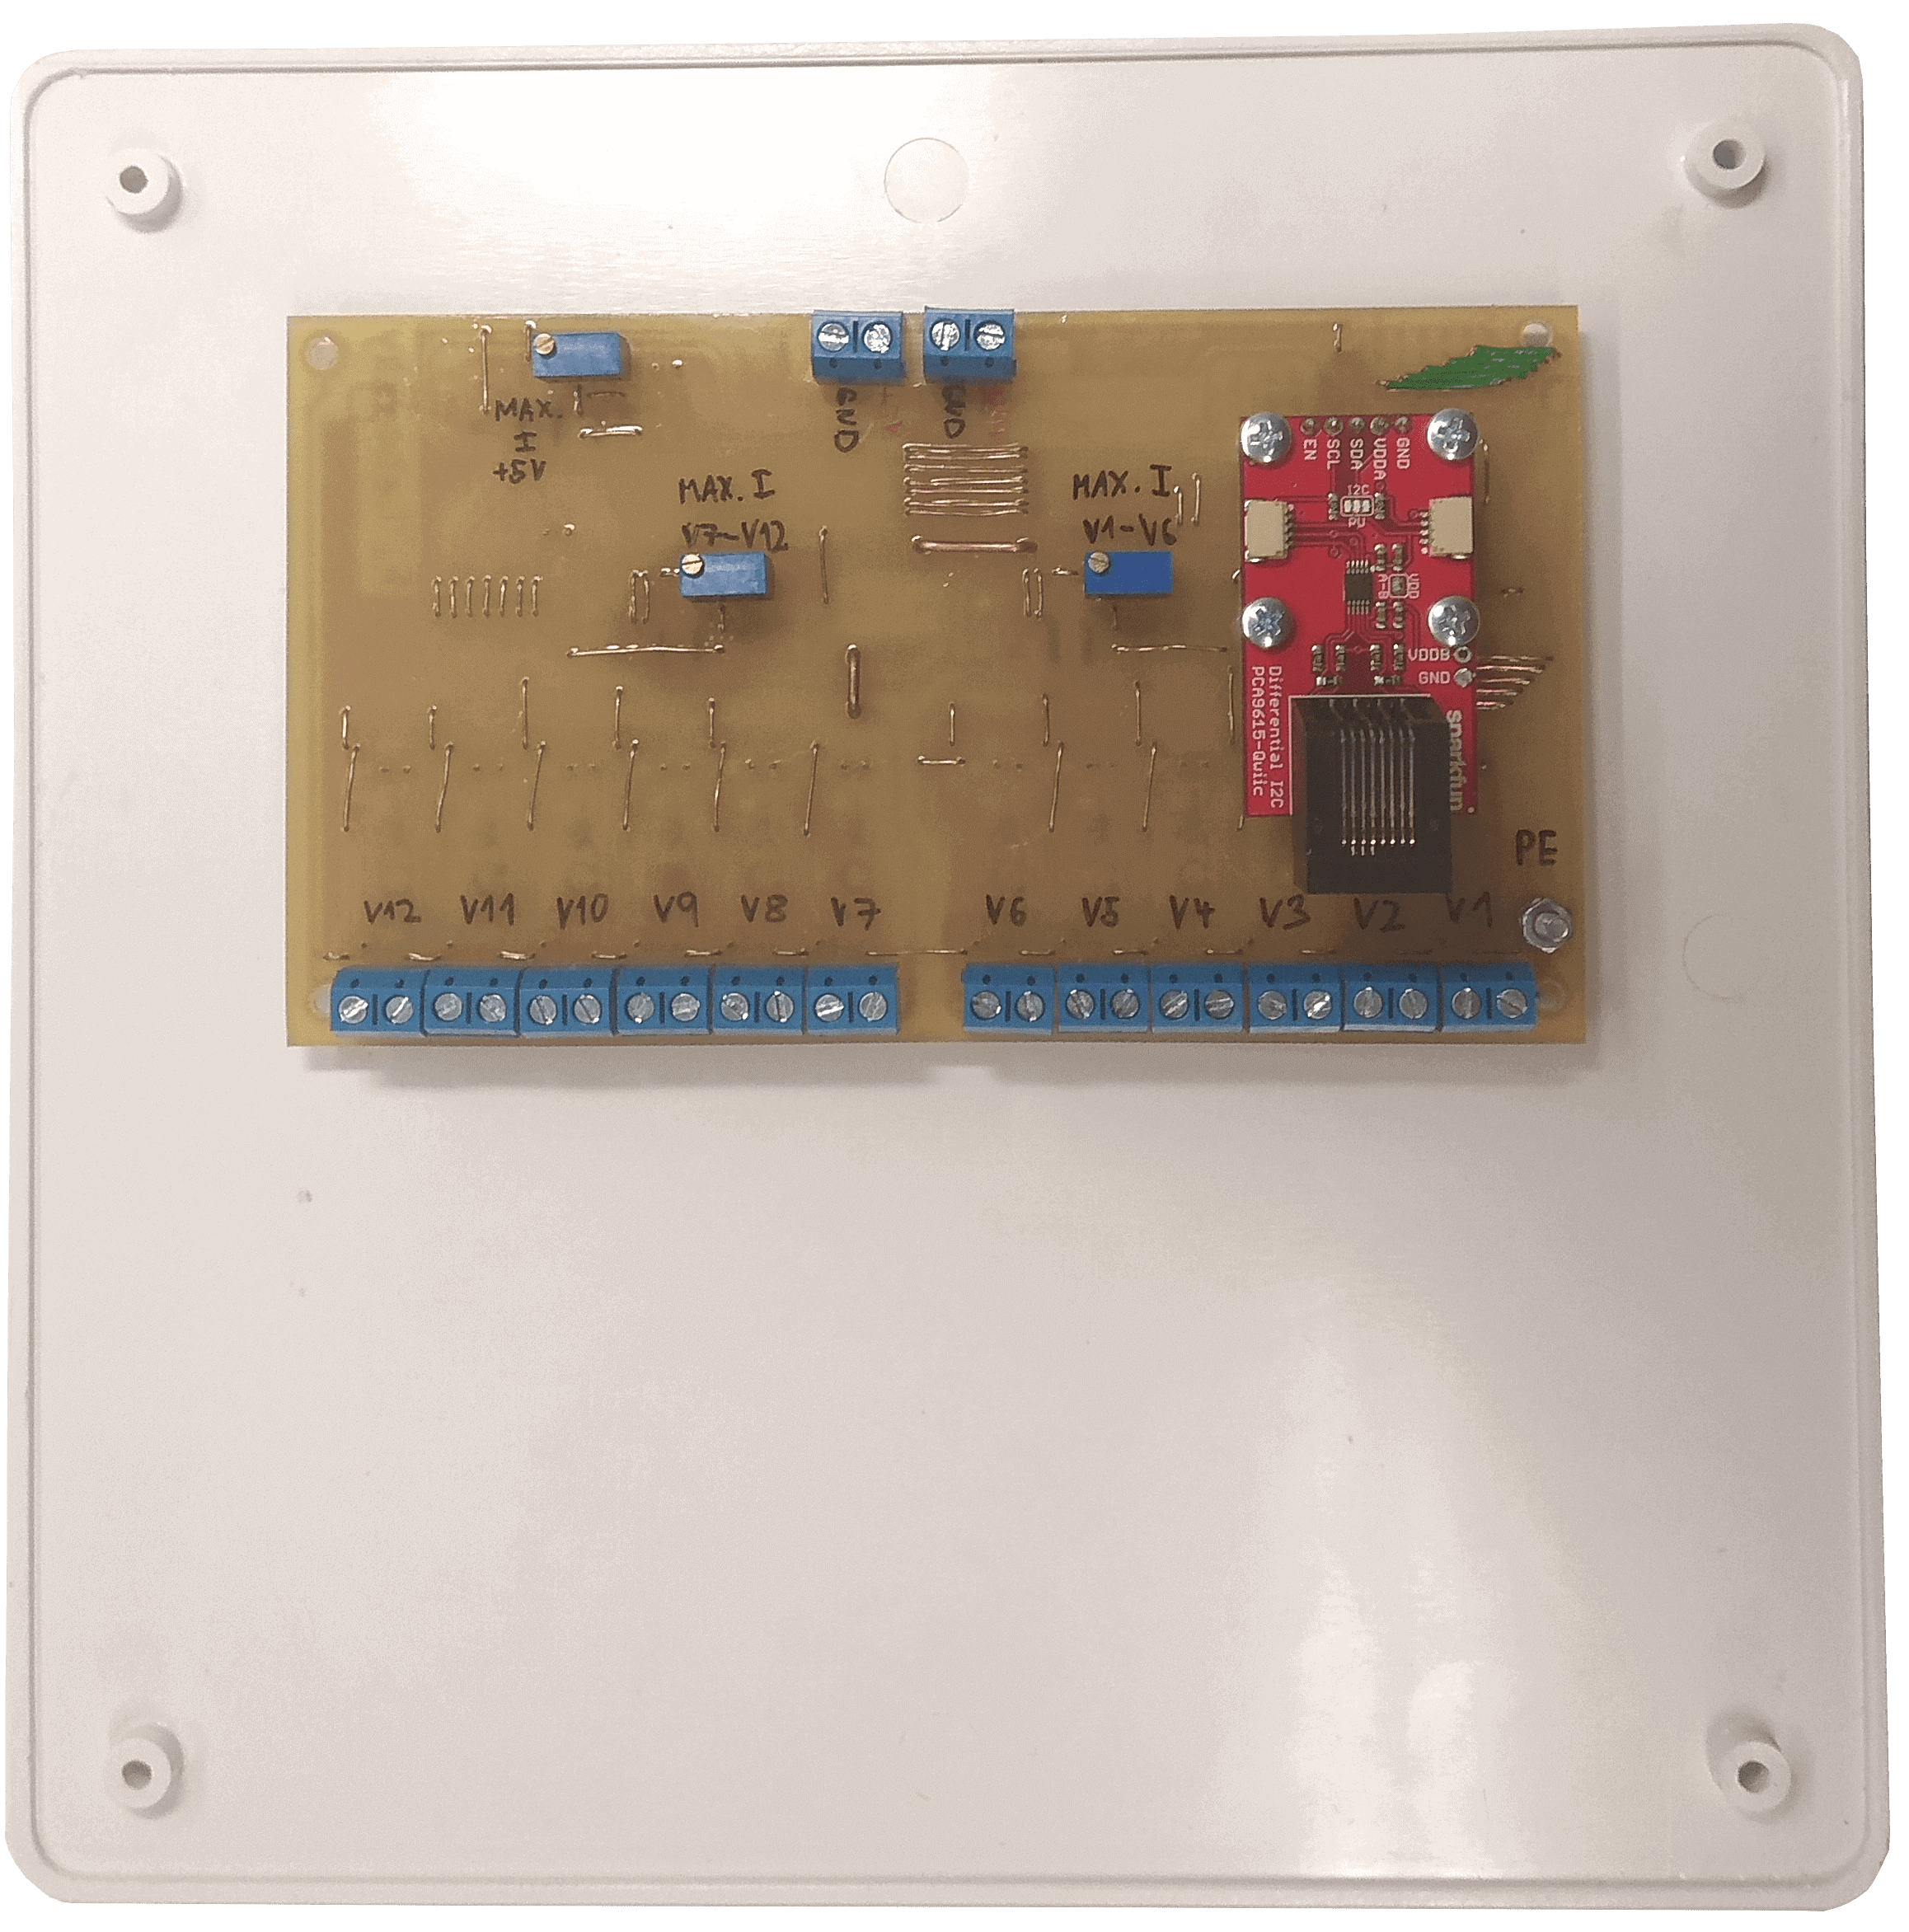
\includegraphics[width=0.95\textwidth]{images/zonovy-regulator/zonovy-regulator-spodni-strana.png}
%    \caption{Zadní část panelu zónového regulátoru.}
%    \label{fig:zonovy-regulator-spodni-strana}
%\end{figure}

%\begin{figure}[H]
%    \centering
%    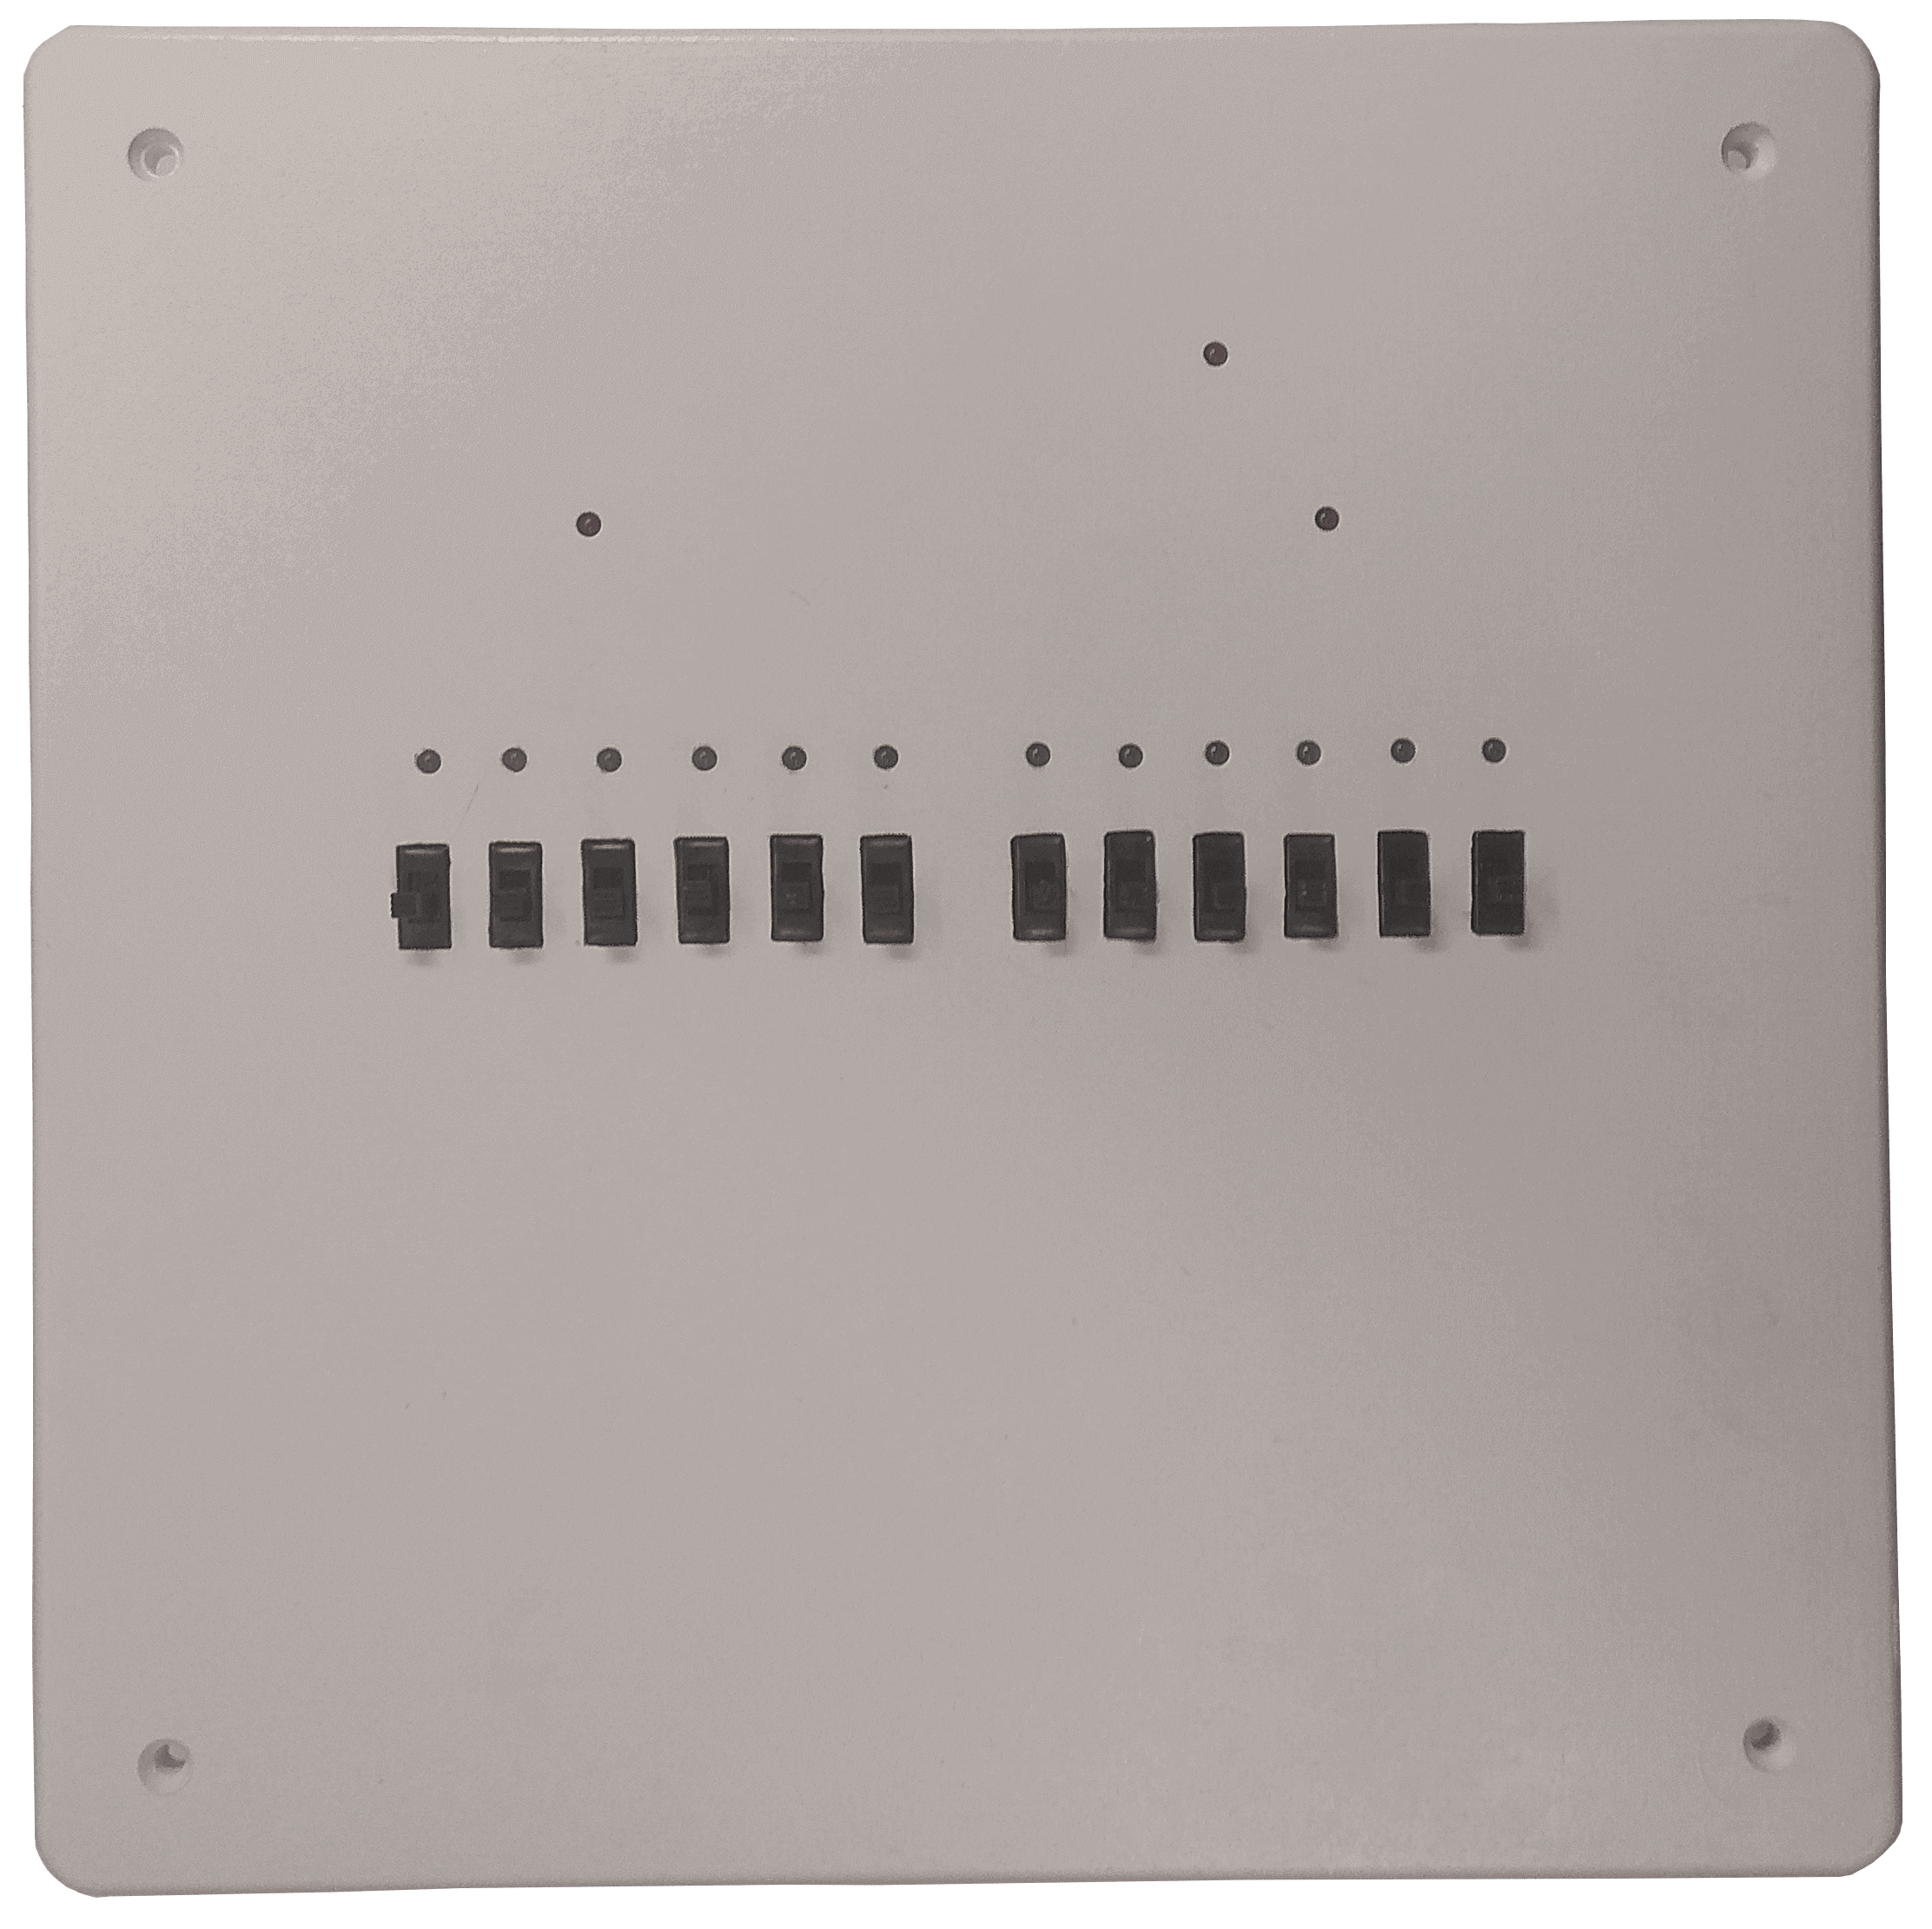
\includegraphics[width=0.95\textwidth]{images/zonovy-regulator/zonovy-regulator-vrchni-strana.png}
%    \caption[Čelní část panelu zónového regulátoru.]{Čelní část panelu zónového regulátoru se signalizačními LED a~manuálním ovládáním pomocí spínačů.}
%    \label{fig:zonovy-regulator-vrchni-strana}
%\end{figure}



\begin{figure}[H]
\centering
\begin{subfigure}{.5\textwidth}
  \centering
  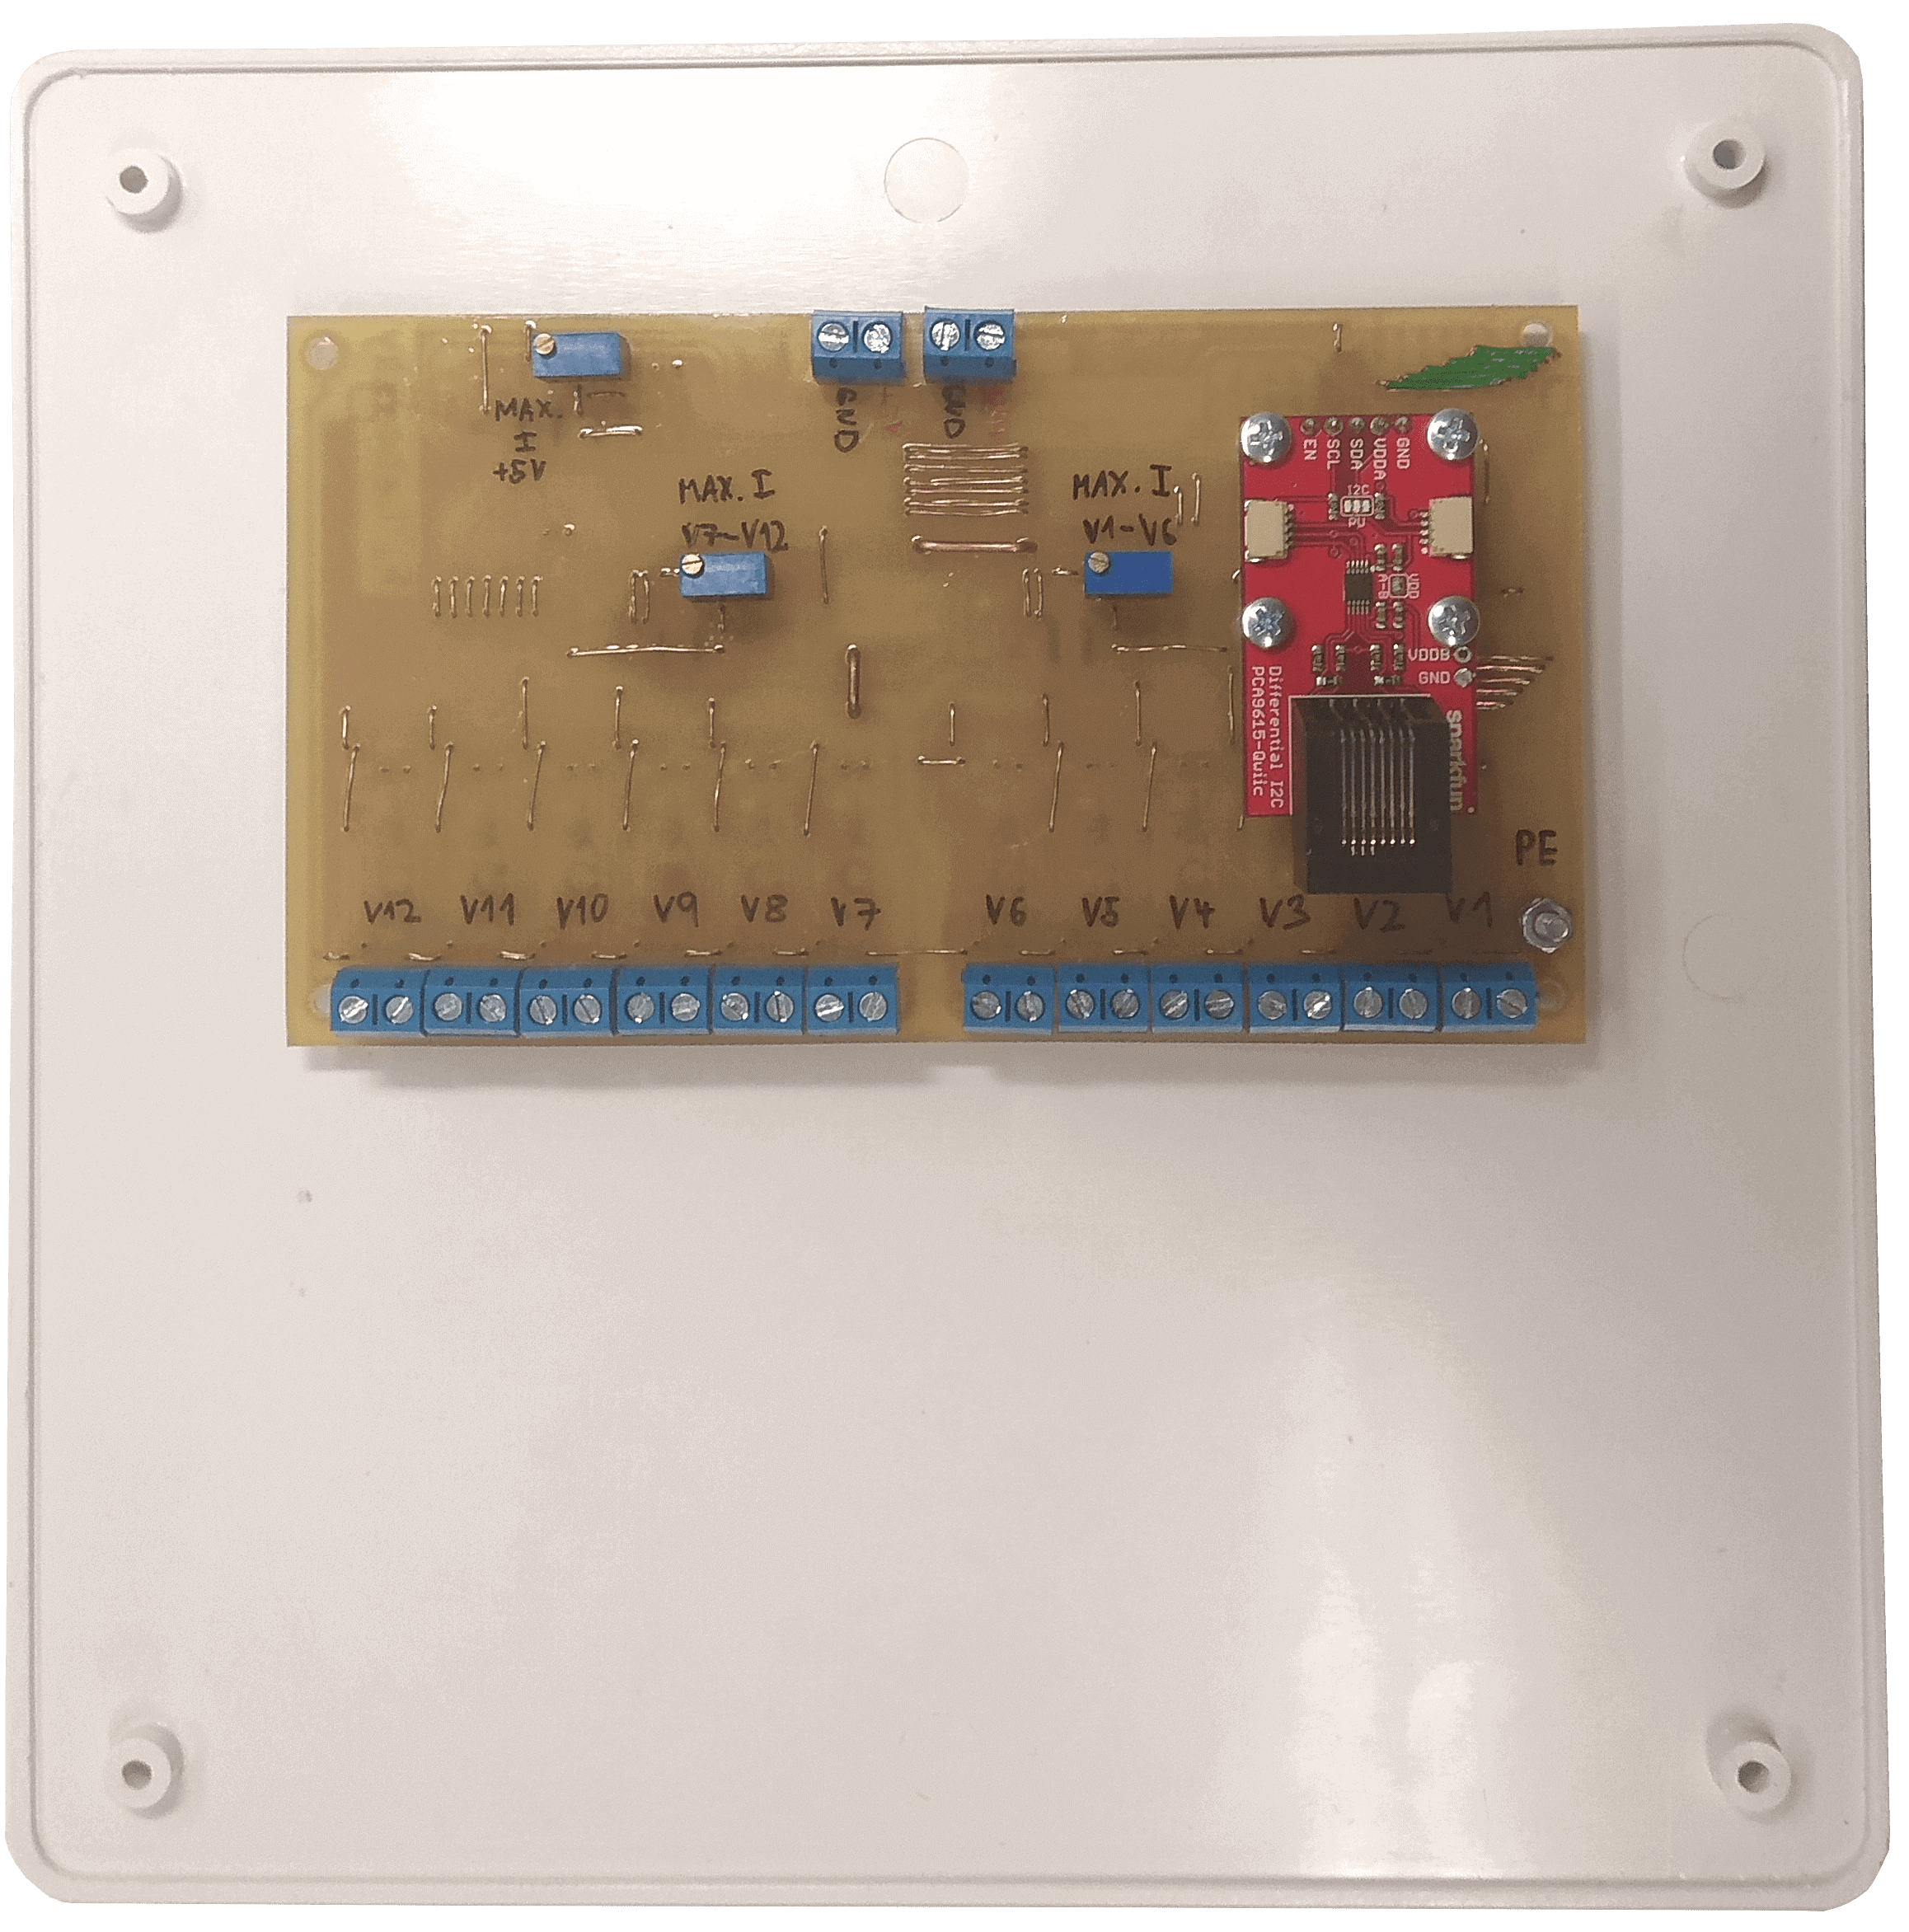
\includegraphics[width=\textwidth]{images/zonovy-regulator/zonovy-regulator-spodni-strana.png}
  \caption{Zadní část panelu zónového regulátoru. \newline \newline}
  \label{fig:zonovy-regulator-spodni-strana}
\end{subfigure}%
\begin{subfigure}{.5\textwidth}
  \centering
  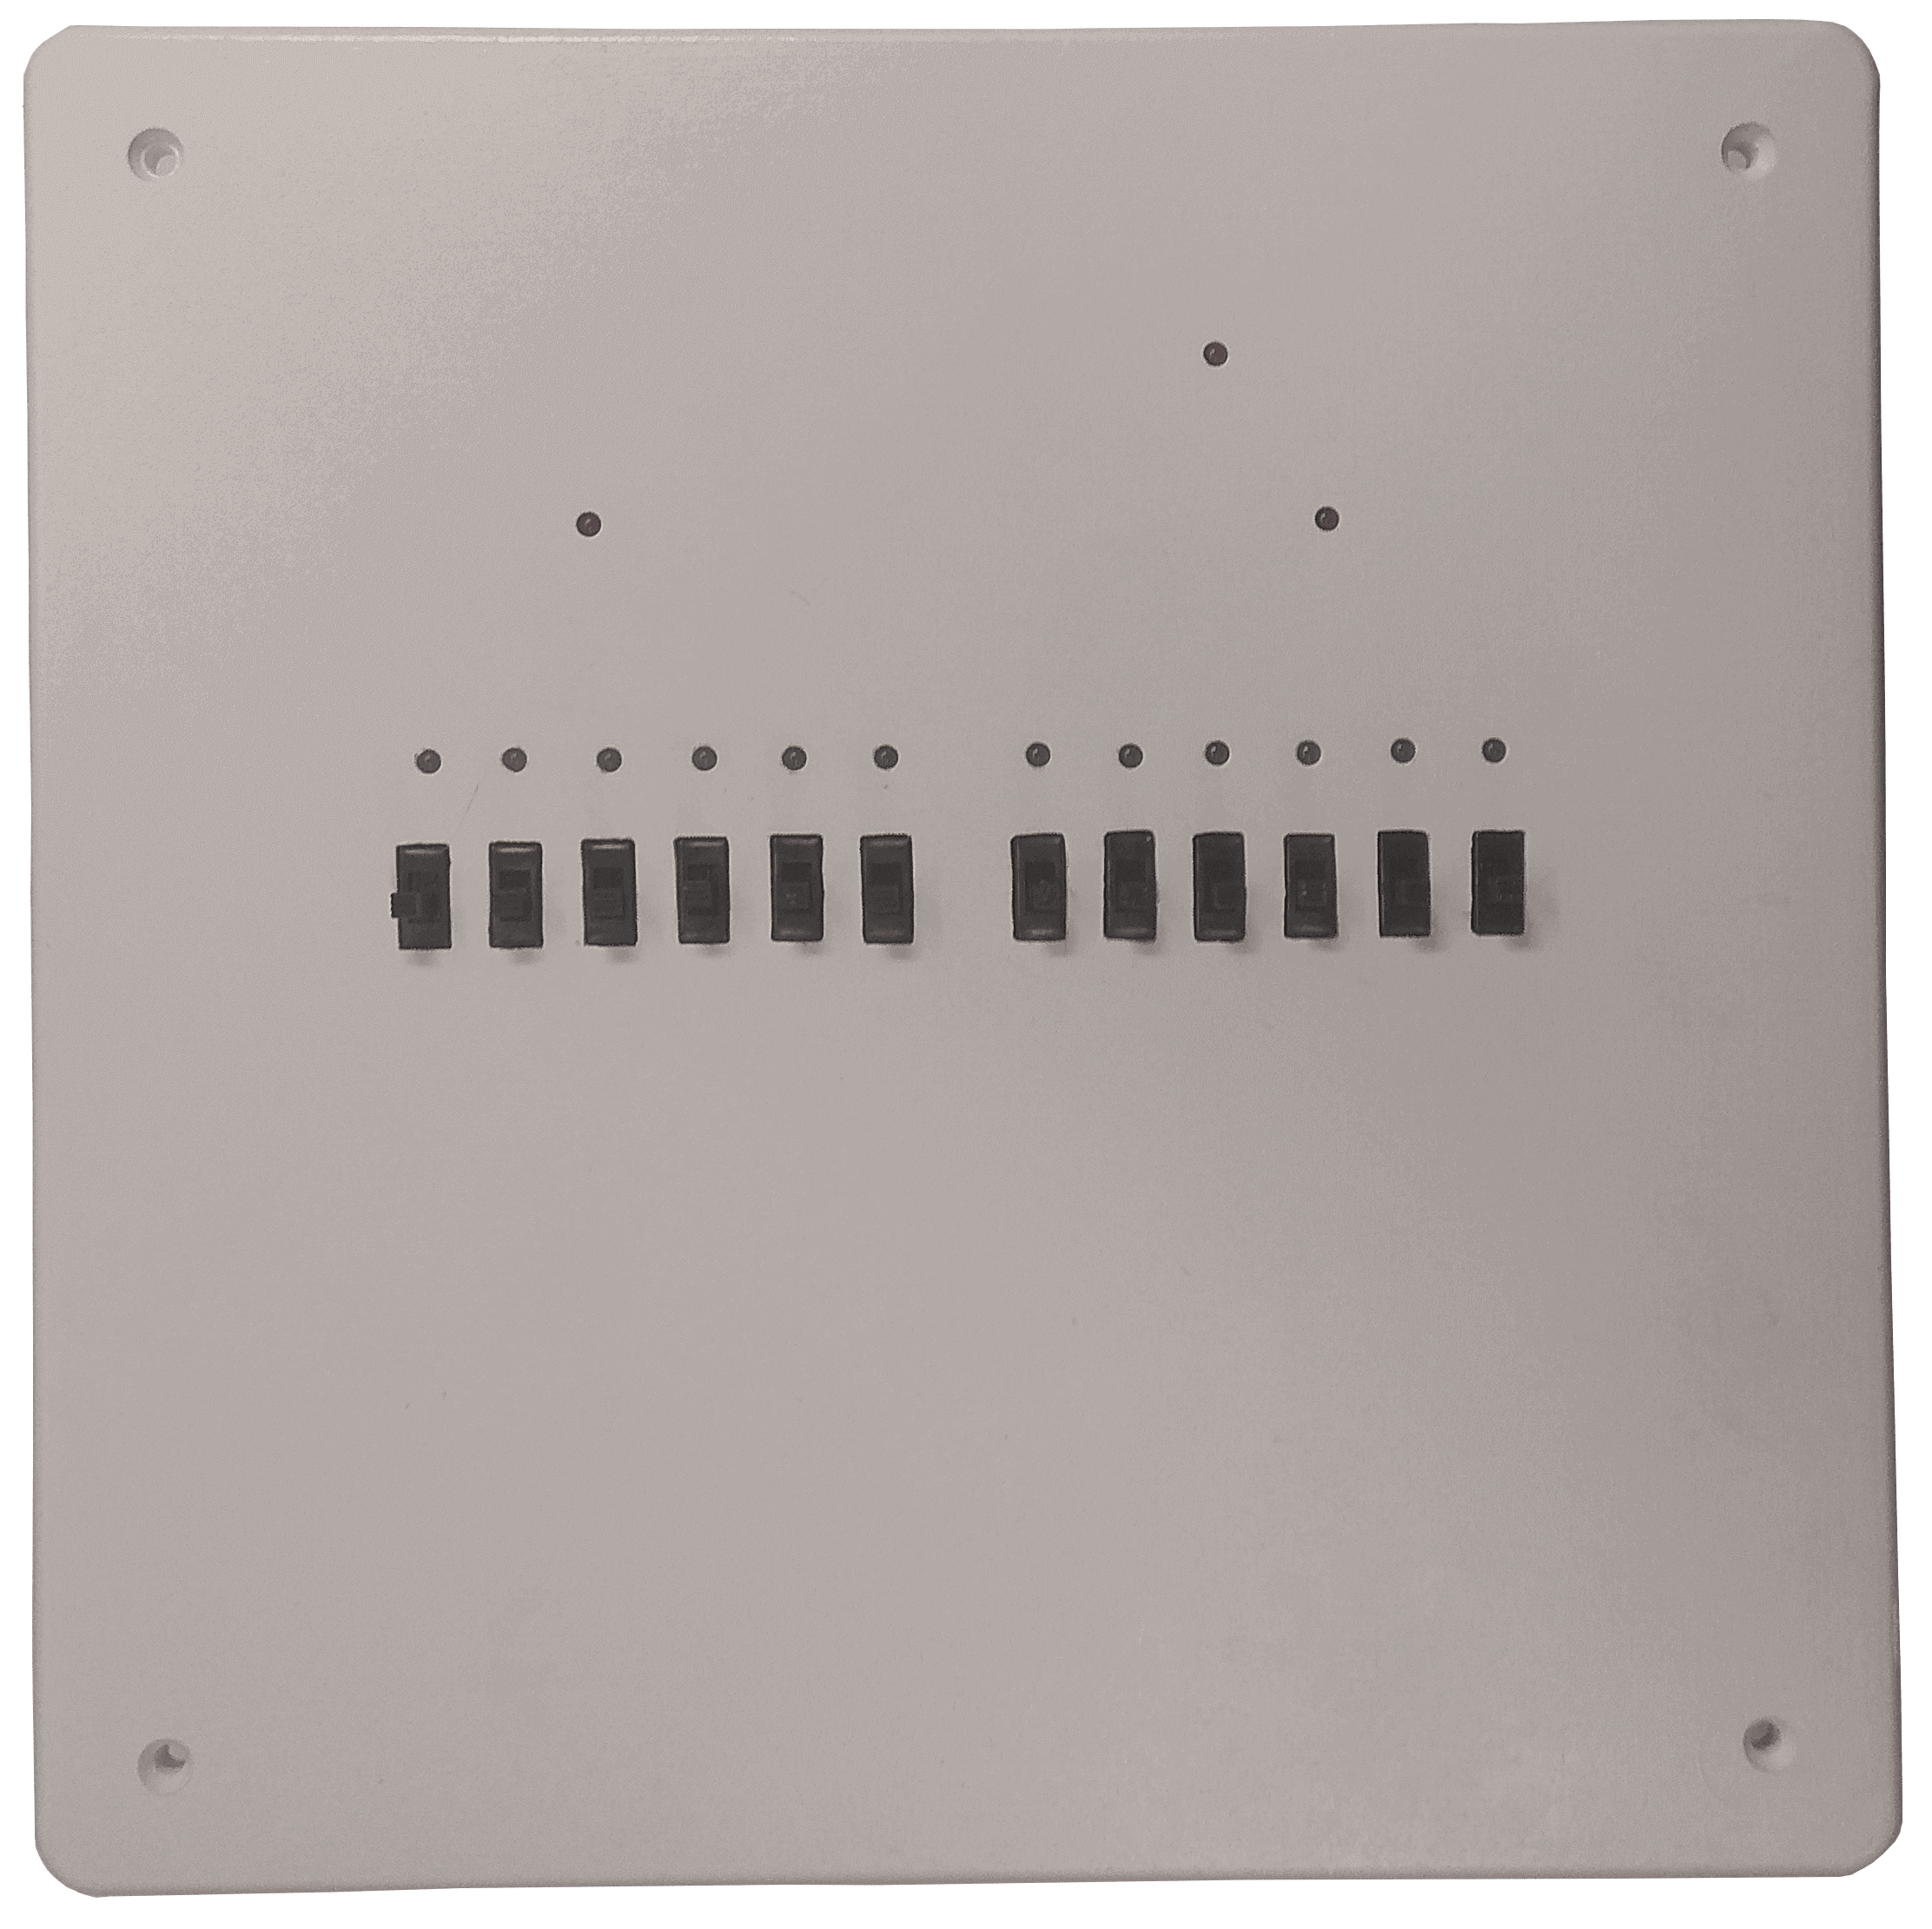
\includegraphics[width=\textwidth]{images/zonovy-regulator/zonovy-regulator-vrchni-strana.png}
  \caption[Čelní část panelu zónového regulátoru.]{Čelní část panelu zónového regulátoru se signalizačními LED a~manuálním ovládáním pomocí spínačů.}
    \label{fig:zonovy-regulator-vrchni-strana}
\end{subfigure}
\caption{Panel pro zónový regulátor.}
\label{fig:zonovy-regulator}
\end{figure}

\subsubsection{Termoelektrické pohony Salus T30NC}  
Termoelektrický pohon Salus T30NC \cite{termoelektricky-pohon-t30nc} slouží k ovládání ventilů pro jednotlivé otopné okruhy. Je napájen stejnosměrným napětí 24 V při maximálním proudovém odběru při zapnutí 250 mA. Provozní příkon jsou 2 W. Rozměr závitu je M30\,×\,1,5. Maximální délka zdvihu pro dřík ventilu činí 4 mm. Síla pohonu je 100 N ($\pm$10 \%). Čas pro otevření je přibližně 2 minuty. Jedná se o~typ \acrshort{nc} (\textit{\acrlong{nc}}). Při odpojení napájení je ventil zavřen. Pohon má funkci „First Open“, neboli je možné pomocí zarážky ventil instalovat jako otevřený bez nutnosti napájení (využít v případě, kdy není ještě instalovaná centrální jednotka). Pro každé patro je použito 12 těchto pohonů.

\begin{figure}[H]
    \centering
    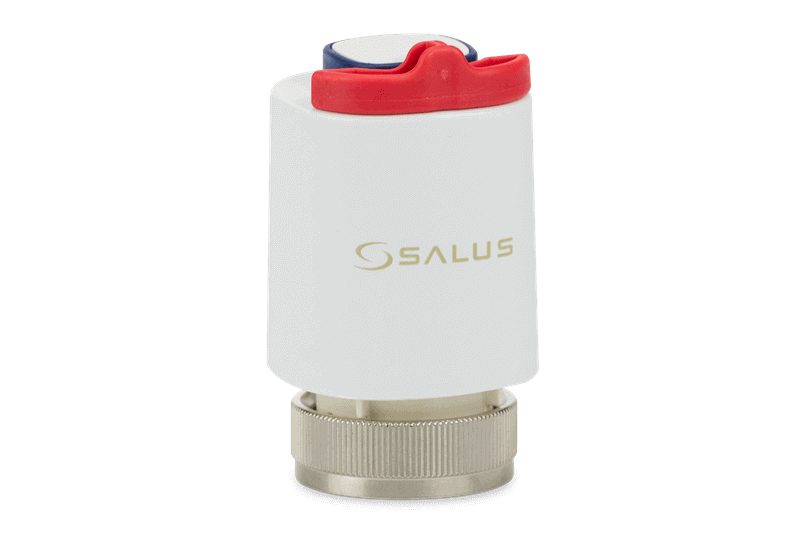
\includegraphics[width=0.5\textwidth]{images/termoelektricky-pohon-salus-t30nc-24-v.png}
    \caption[Termoelektrický pohon Salus T30NC.]{Termoelektrický pohon Salus T30NC na stejnosměrné napětí 24~V \cite{termoelektricky-pohon-t30nc}.}
    \label{fig:termoelektricky-pohon-salus-t30nc-24-v}
\end{figure}

\section{Digitální chodbové termostaty}
\label{sec:digitalni-chodbove-termostaty}
\begin{figure}[H]
   \centering
   \def\svgwidth{0.4\columnwidth}
   \input{images/svg/otopna-soustava/vyrez-lokalni-termostaty.pdf_tex}
    \caption[Výřez pro umístění chodbových termostatů.]{Výřez z obrázku \ref{fig:otopna-soustava-a-elektronika-rez-domu} – umístění chodbových termostatů.}
    \label{fig:vyrez-lokalni-termostaty}
\end{figure}

Na obrázku \ref{fig:vyrez-lokalni-termostaty} je výřez části z celkového nákresu (obrázek \ref{fig:otopna-soustava-a-elektronika-rez-domu}) systému znázorňující umístění chodbových termostatů. Pro snímání teplot z jednotlivých pater na chodbách slouží zakoupené digitální termostaty s označením W3230 \cite{digitalni-termostat-w3230}. Termostat disponuje jedním spínací výstupem (v~případě potřeby vytápění se výstup sepne, jinak je rozepnut). Je možné nastavit hysterezi, časové zpoždění, kalibraci teploty a rozsah maximálních teplot. Lze také aktivovat signalizaci, která se spustí po dosažení maximální přípustné teploty. Pro napájení je potřeba stejnosměrné napětí 12~V. Pro snímání teploty slouží  \acrshort{ntc} (\textit{\acrlong{ntc}}) termistor. Rozsah teplot je -40 °C až 120 °C. Přesnost měření je $\pm$ 0,1 °C. Termostat lze nahradit za jakýkoliv jiný, který disponuje spínacím výstupem.


\begin{figure}[H]
    \centering
    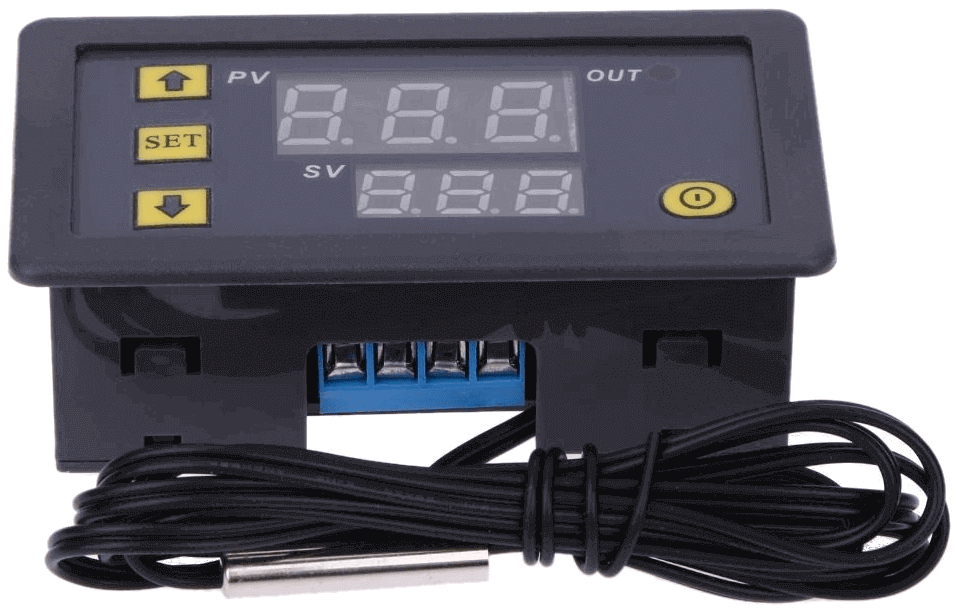
\includegraphics[width=0.5\textwidth]{images/digitalni-termostat-w3230.png}
    \caption[Digitální chodbový termostat W3230.]{Digitální chodbový termostat W3230 \cite{digitalni-termostat-w3230}.}
    \label{fig:digitalni-termostat-w3230}
\end{figure}

\section{Spínací jednotka}
\begin{figure}[H]
   \centering
   \def\svgwidth{0.4\columnwidth}
   \input{images/svg/otopna-soustava/vyrez-spinaci-jednotka.pdf_tex}
    \caption[Umístění spínacích jednotek.]{Výřez z obrázku \ref{fig:otopna-soustava-a-elektronika-rez-domu}. Umístění spínacích jednotek.}
    \label{fig:vyrez-spinaci-jednotka}
\end{figure}
Na obrázku \ref{fig:vyrez-spinaci-jednotka} je výřez části z celkového nákresu (obrázek \ref{fig:otopna-soustava-a-elektronika-rez-domu}) systému znázorňující umístění spínacích jednotek. Pro spínání čerpadel a signalizačních LED slouží dva zakoupené relé moduly po čtyřech kanálech. Relé umožňují spínat výkony 250 VAC při max. 10~A a 30 V DC při max. 10~A. Jednotlivé kanály jsou oddělené galvanicky (dále je vyfrézovaná část DPS mezi výkonovou částí a spínací částí), též je možné využít různých zdrojů pro napájení spínací části a napájení relé. Zapojení jednoho kanálu je v příloze \ref{app:schemata-ostatni}. Celý relé modul je na obrázku \ref{fig:ctyr-kanalovy-rele-modul}. Pro spínání síťového napětí je použit jeden relé modul, pro spínání slaboproudého napětí (LED diody, kotel) je použit druhý relé modul.

%\begin{figure}[H]
%    \centering
%    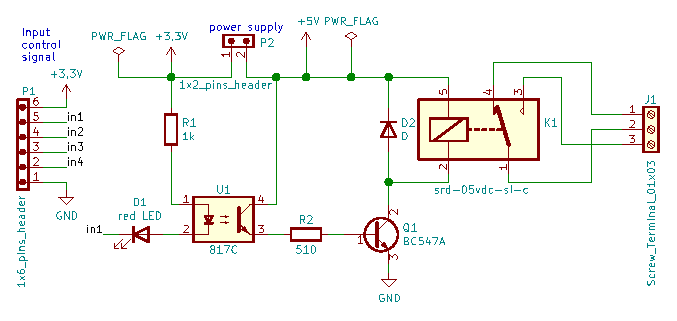
\includegraphics[width=\textwidth]{images/svg/kicad/rele-modul-jeden-kanal.eps}
%    \caption{Zapojení jednoho kanálu relé modulu.}
%    \label{fig:rele-modul-jeden-kanal}
%\end{figure}


\begin{figure}[H]
    \centering
    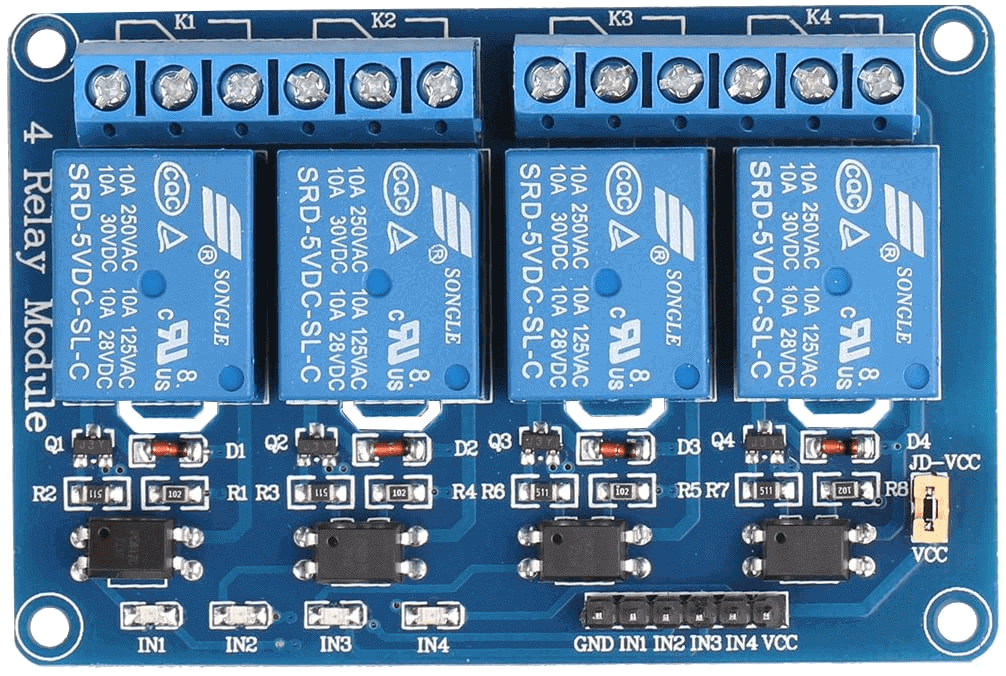
\includegraphics[width=0.5\textwidth]{images/ctyr-kanalovy-rele-modul.png}
    \caption[Čtyř kanálový relé modul.]{Čtyř kanálový relé modul \cite{ctyr-kanalovy-rele-modul}.}
    \label{fig:ctyr-kanalovy-rele-modul}
\end{figure}

\section{Realizovaný rozvaděč s~elektronikou}
\begin{figure}[H]
   \centering
   \def\svgwidth{0.5\columnwidth}
   \input{images/svg/otopna-soustava/vyrez-rozvadec.pdf_tex}
    \caption[Výřez pro umístění rozvaděče s elektronikou.]{Výřez z obrázku \ref{fig:otopna-soustava-a-elektronika-rez-domu} – umístění rozvaděče s elektronikou.}
    \label{fig:vyrez-rozvadec}
\end{figure}

Na obrázku \ref{fig:vyrez-rozvadec} je výřez části z celkového nákresu (obrázek \ref{fig:otopna-soustava-a-elektronika-rez-domu}) pro rozvaděč s elektronikou. V realizovaném rozvaděči na obrázku \ref{fig:rozvadec-ve-sklepe-s-elektronikou} je umístěn 5 V zdroj pro napájení centrální jednotky, relé modulů, I$^2$C diferenciální sběrnice, napájení 1-Wire sběrnice, napájení elektroniky u krbů a napájení pro zónové regulátory. Dále je zde 12 V zdroj pro napájení dvou chodbových termostatů. Zdroj 24 V pro zónové regulátory, respektive pro napájení termoelektrických pohonů. V  neposlední řadě jsou zde jističe pro jednotlivé zdroje a čerpadla včetně proudového chrániče.

\begin{figure}[H]
    \centering
    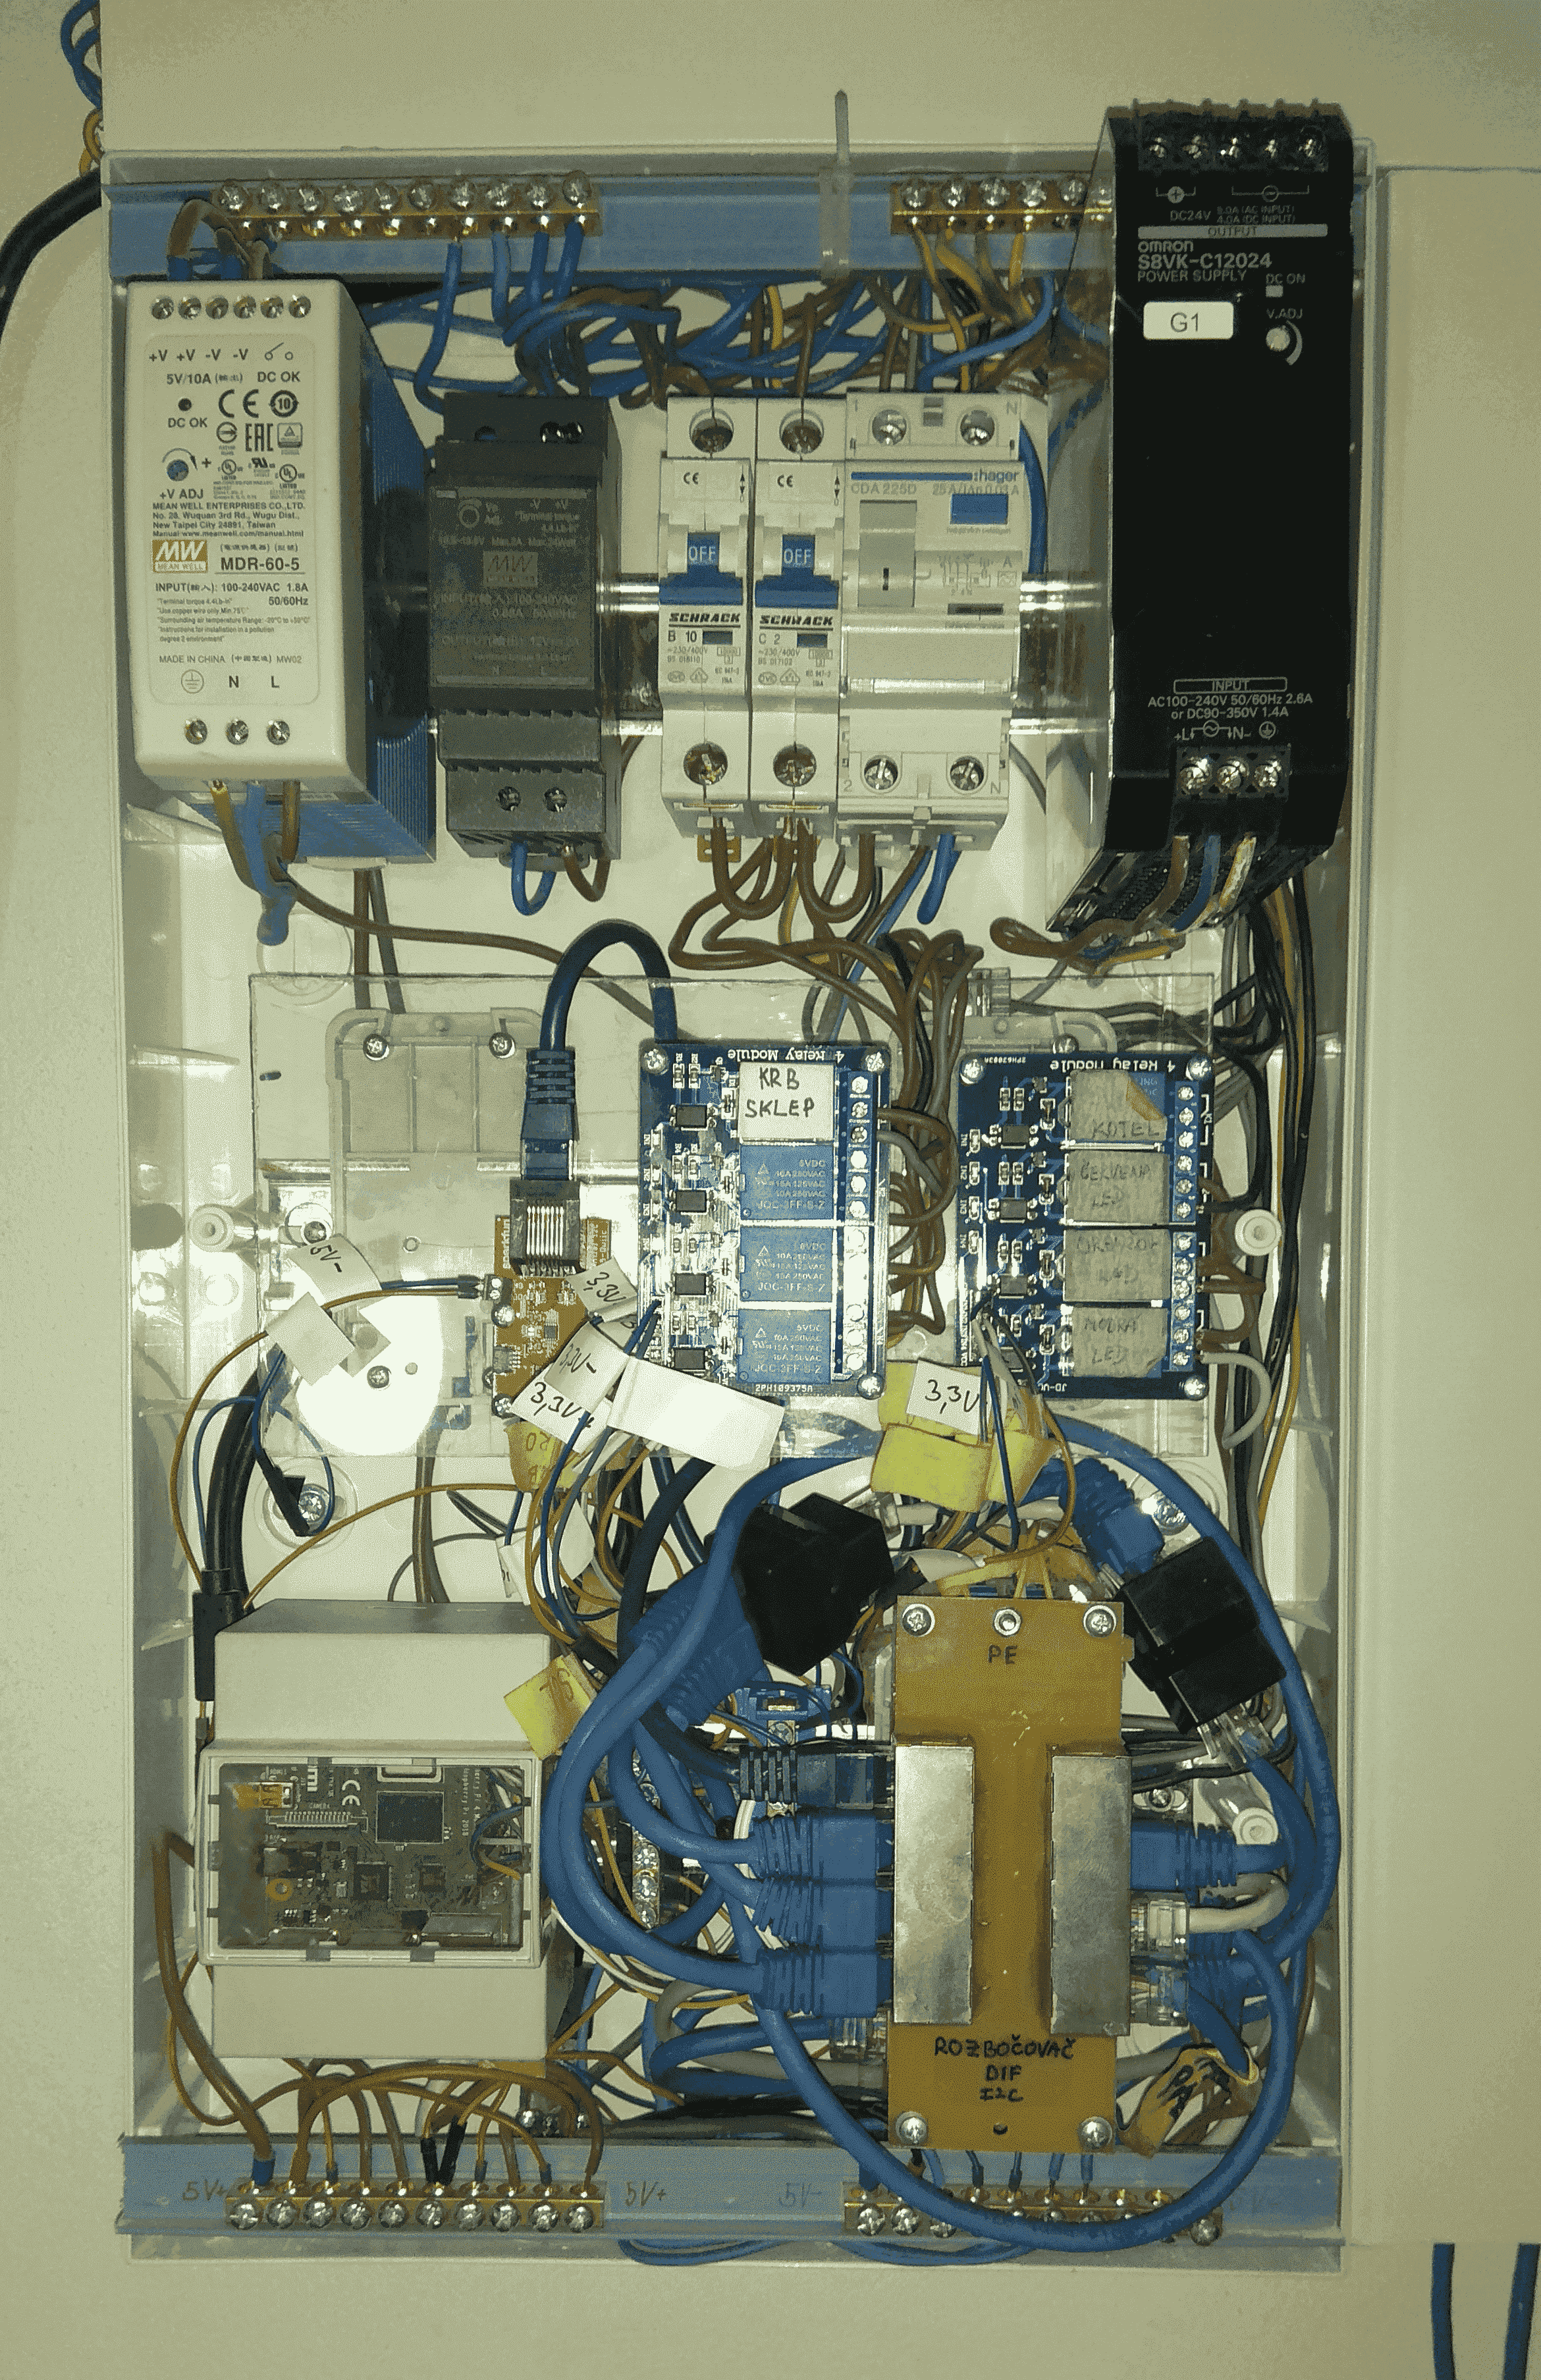
\includegraphics[width=\textwidth]{images/rozvadec-ve-sklepe-s-elektronikou.png}
    \caption{Realizovaný rozvaděč s~elektronikou.}
    \label{fig:rozvadec-ve-sklepe-s-elektronikou}
\end{figure}


\section{Nástěnný snímač prostorové teploty}

Pro snímání prostorové teploty z místností slouží nástěnný snímač prostorové teploty (dále jen zkráceně snímací jednotka). Tyto snímací jednotky tedy primárně slouží k měření teploty a její následné odesílání do centrální jednotky. Dále disponují tlačítky pro nastavení požadované teploty (změna teploty s~krokem 0,5 °C) pro danou místnost. Aktuálně naměřenou a požadovanou teplotu zobrazují uživateli přímo na displeji. V případě přenastavení v centrálním systému, dojde k propsání těchto změn přímo na jednotlivé snímací jednotky. Snímací jednotky měří teplotu v místnosti každých 30~sekund. V případě síťového výpadku komunikace se zařízení automaticky snaží připojení obnovit, samotný výpad je signalizován i v centrální jednotce. Jednotky existují ve dvou variantách. První varianta komunikace s centrální jednotkou pomocí Ethernetu a je napájena pomocí aktivního \acrshort{poe} (\textit{\acrlong{poe}}). Druhá varianta komunikuje s centrální jednotkou pomocí bezdrátové sítě WiFi a je napájena pomocí síťového adaptéru. Obě varianty jsou popsány níže v sekci \ref{sec:ethernet-modul} a \ref{sec:wifi-modul}. Celkově je po domě umístěno 6 zařízení s Ethernetem a~4 zařízení s WiFi.

\subsection{Varianta s Ethernetem}
\label{sec:ethernet-modul}

Na obrázku \ref{fig:blokove-schema-nastenny-snimac-teploty-ethernet} je blokové schéma nástěnného snímače prostorové teploty komunikující pomocí Ethernetu a je napájen pomocí aktivního POE. Snímač je napájen ze zařízení \acrshort{pse} (\textit{\acrlong{pse}}), které řídí vykomunikování napájení a výkonnostní třídy pro koncové zařízení (snímač (\acrshort{pd} (\textit{\acrlong{pd}}))). Jak zařízení PSE, tak PD podporují standart 802.3af respektive 802.3at. Zařízení PD jsou nastavená pro nejnižší definovanou výkonovou třídu 1 (max. výkon PSE pro jednotlivé PD zařízení je 4 W). Pro přenos napětí se využívají tzv. fantomové napětí, kdy v případě využití páru 1,2 a 3,6 se stejnosměrné napětí vyvede ze středu transformátoru. Další možností je využití volných párů 4,5 a 7,8 (zejména při rychlosti 10 nebo 100~Mbit/s (využity pro přenos dat 2 páry)). Vstupní napětí z PSE (44–57 V v~závislosti na délce kabelu UTP a ztrátách) prochází přes diodový usměrňovač (nezávislost kladného pólu zdroje a země). Je zde řídící obvod TPS23753A, který zajišťuje komunikaci/rozhraní pro správné nastavení a povolení napětí z PSE, dále zajišťuje řízení převodu vstupního napětí na výstupní napětí 5~V (DC-DC měnič), je zapojen v topologie Flyback (využívá tedy vázaný induktor). Zpětná vazba je řešena pomocí optické zpětné vazby s nastavitelnou Zenerovou diodou TLV431A v zapojení komparátoru. 

Zařízení je možné tedy napájet pomocí 5 V z POE nebo při připojení USB respektive modulu, ke kterému je připojené USB. V případě, že je k~dispozici POE, dojde zablokování napájení z USB (pomocí MOSFETu s~kanálem P). Napětí 5 V je následně vedeno do dvou \acrshort{ldo} (\textit{\acrlong{ldo}}) regulátorů. Jeden slouží pouze pro napájení ESP32 modulu, druhá je pro napájení zbylých periferií (displej, tlačítka, teplotní senzor, obvod pro fyzickou vrstvu Ethernetu W5500). Důvodem rozdělení je proudové rozdělení jednotlivých regulátorů a tedy i jejich ztrátové teplo. Vzhledem k parametrům udávané výrobcem modulu ESP32 je možné max. proudový odběr až 0,5~A (proto byl vybrán regulátor, který toto zatížení dlouhodobě zvládne při daném úbytku napětí i když se reálně nepředpokládá, že k tomuto zatížení dojde). Dále bylo zohledněno, pokud by došlo k ESD události (jedná se o~zařízení na které uživatelé sahají), tak je žádoucí aby došlo maximálně k~restartu periferií a ne k restartu samotného ESP32 modulu. 

Pro programování modulu je zde konektor pro připojení externího modulu (viz sekce ), kde jsou piny pro TX/RX signál z UART a signály na automatický reset a boot modulu a piny pro napájení 5 V a země. Dále jsou zde přímo na DPS umístěné tlačítka pro boot a reset ESP32 modulu bez závislosti připojení programovacího modulu (lze tedy programovat i jinými moduly, které nemají automatický reset a boot). 

Samotné zařízení disponujeme ohranými transily na místech konektorů a připojených zařízení, které jsou přímo v kontaktu s uživatelem. Samotný obvod pro POE též disponuje proudovou a teplotní ochranou. LDO regulátory disponují detekcí nízkého vstupního napětí pro úspěšné spuštění, teplotní pojistkou a ochranou při zvýšení výstupního napětí vůči vstupnímu. 

Pro zobrazování aktuální a požadované teploty jsem zvolil barevný TFT displej velikosti 2.2" (240×320 pixelů) s řadičem ILI9341. Displej je připojen k~ESP32 modulu pomocí SPI sběrnice. Displej též disponuje možností ovládání podsvícení pomocí PWM, tento řídící pin je připojen též k modulu. Pro fyzickou vrstvu slouží obvod W5500, který implementuje ethernetový řadič s integrovaným TCP/IP. Obvod je s modulem ESP32 připojen pomocí SPI sběrnice. Pro snímání teploty slouží teplotní senzor DS18B20 (viz sekce \ref{sec:teplotni-senzory-pro-krby}). V neposlední řadě jsou zde tři tlačítka pro nastavení požadované teploty a~vyvolání nabídky menu.

Modul ESP32 disponuje rozhraním \acrshort{rmii} (\textit{\acrlong{rmii}})  nicméně ke složitější implementaci a většímu počtu pinů. Jsem zvolil integrovaný obvod W5500. Použití i využití následných knihoven bylo mnohem jednodušší. Vzhledem k malému vytížení komunikace je tento obvod dostačující. Pro komunikace mezi modulem ESP32 a displejem a obvodem W5500 jsou využity dvě nezávislé SPI sběrnice. 

V příloze \ref{app:nastenny-snimac-prostorove-teploty-ethernet} je schéma snímací jednotky. Na obrázku \ref{fig:dps-nastenny-snimac-prostorove-teploty-ethernet-vrchni-cast} je vrchní část realizované DPS pro snímací jednotku. Pro lepší galvanické oddělení jsou vyfrézované drážky. Dále na obrázku \ref{fig:dps-nastenny-snimac-prostorove-teploty-ethernet-vrchni-cast-displej} je DPS s osazeným displejem. Na obrázku \ref{fig:dps-nastenny-snimac-prostorove-teploty-ethernet-spodni-cast} je spodní část DPS. Kompletní zařízení včetně umístění do krabičky a popis samotné krabičky je v části \ref{sec:krabicka-pro-nastenny-snimac-prostorove-teploty}.

\begin{figure}[H]
    \centering
    \def\svgwidth{\columnwidth}
    \input{images/svg/blokove-schema-nastenny-snimac-teploty-ethernet.pdf_tex}
    \caption[]{Blokové schéma nástěnného snímače prostorové teploty s Ethernetem.}
    \label{fig:blokove-schema-nastenny-snimac-teploty-ethernet}
\end{figure}

\begin{figure}[H]
    \centering
    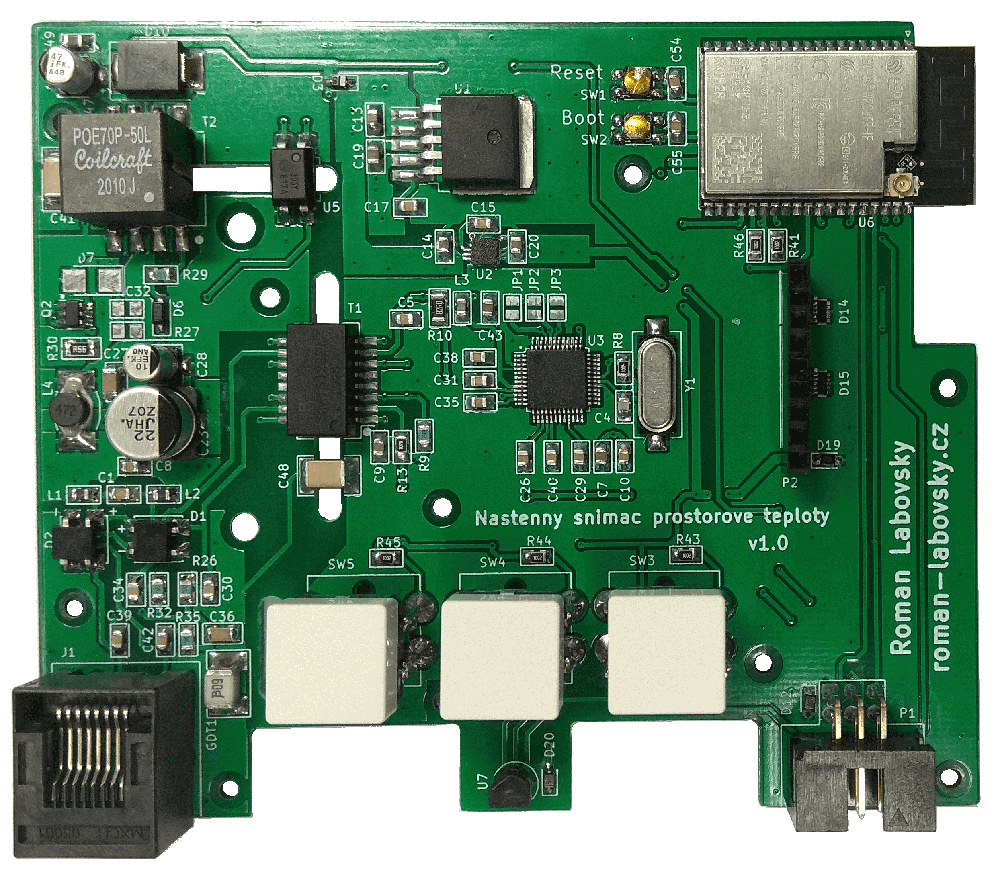
\includegraphics[width=0.89\textwidth]{images/nastenny-snimac-prostorove-teploty-ethernet/dps-nastenny-snimac-prostorove-teploty-ethernet-vrchni-cast.png}
    \caption{DPS nástěnného snímače prostorové teploty s Ethernetem, vrchní strana.}
    \label{fig:dps-nastenny-snimac-prostorove-teploty-ethernet-vrchni-cast}
\end{figure}

\begin{figure}[H]
    \centering
    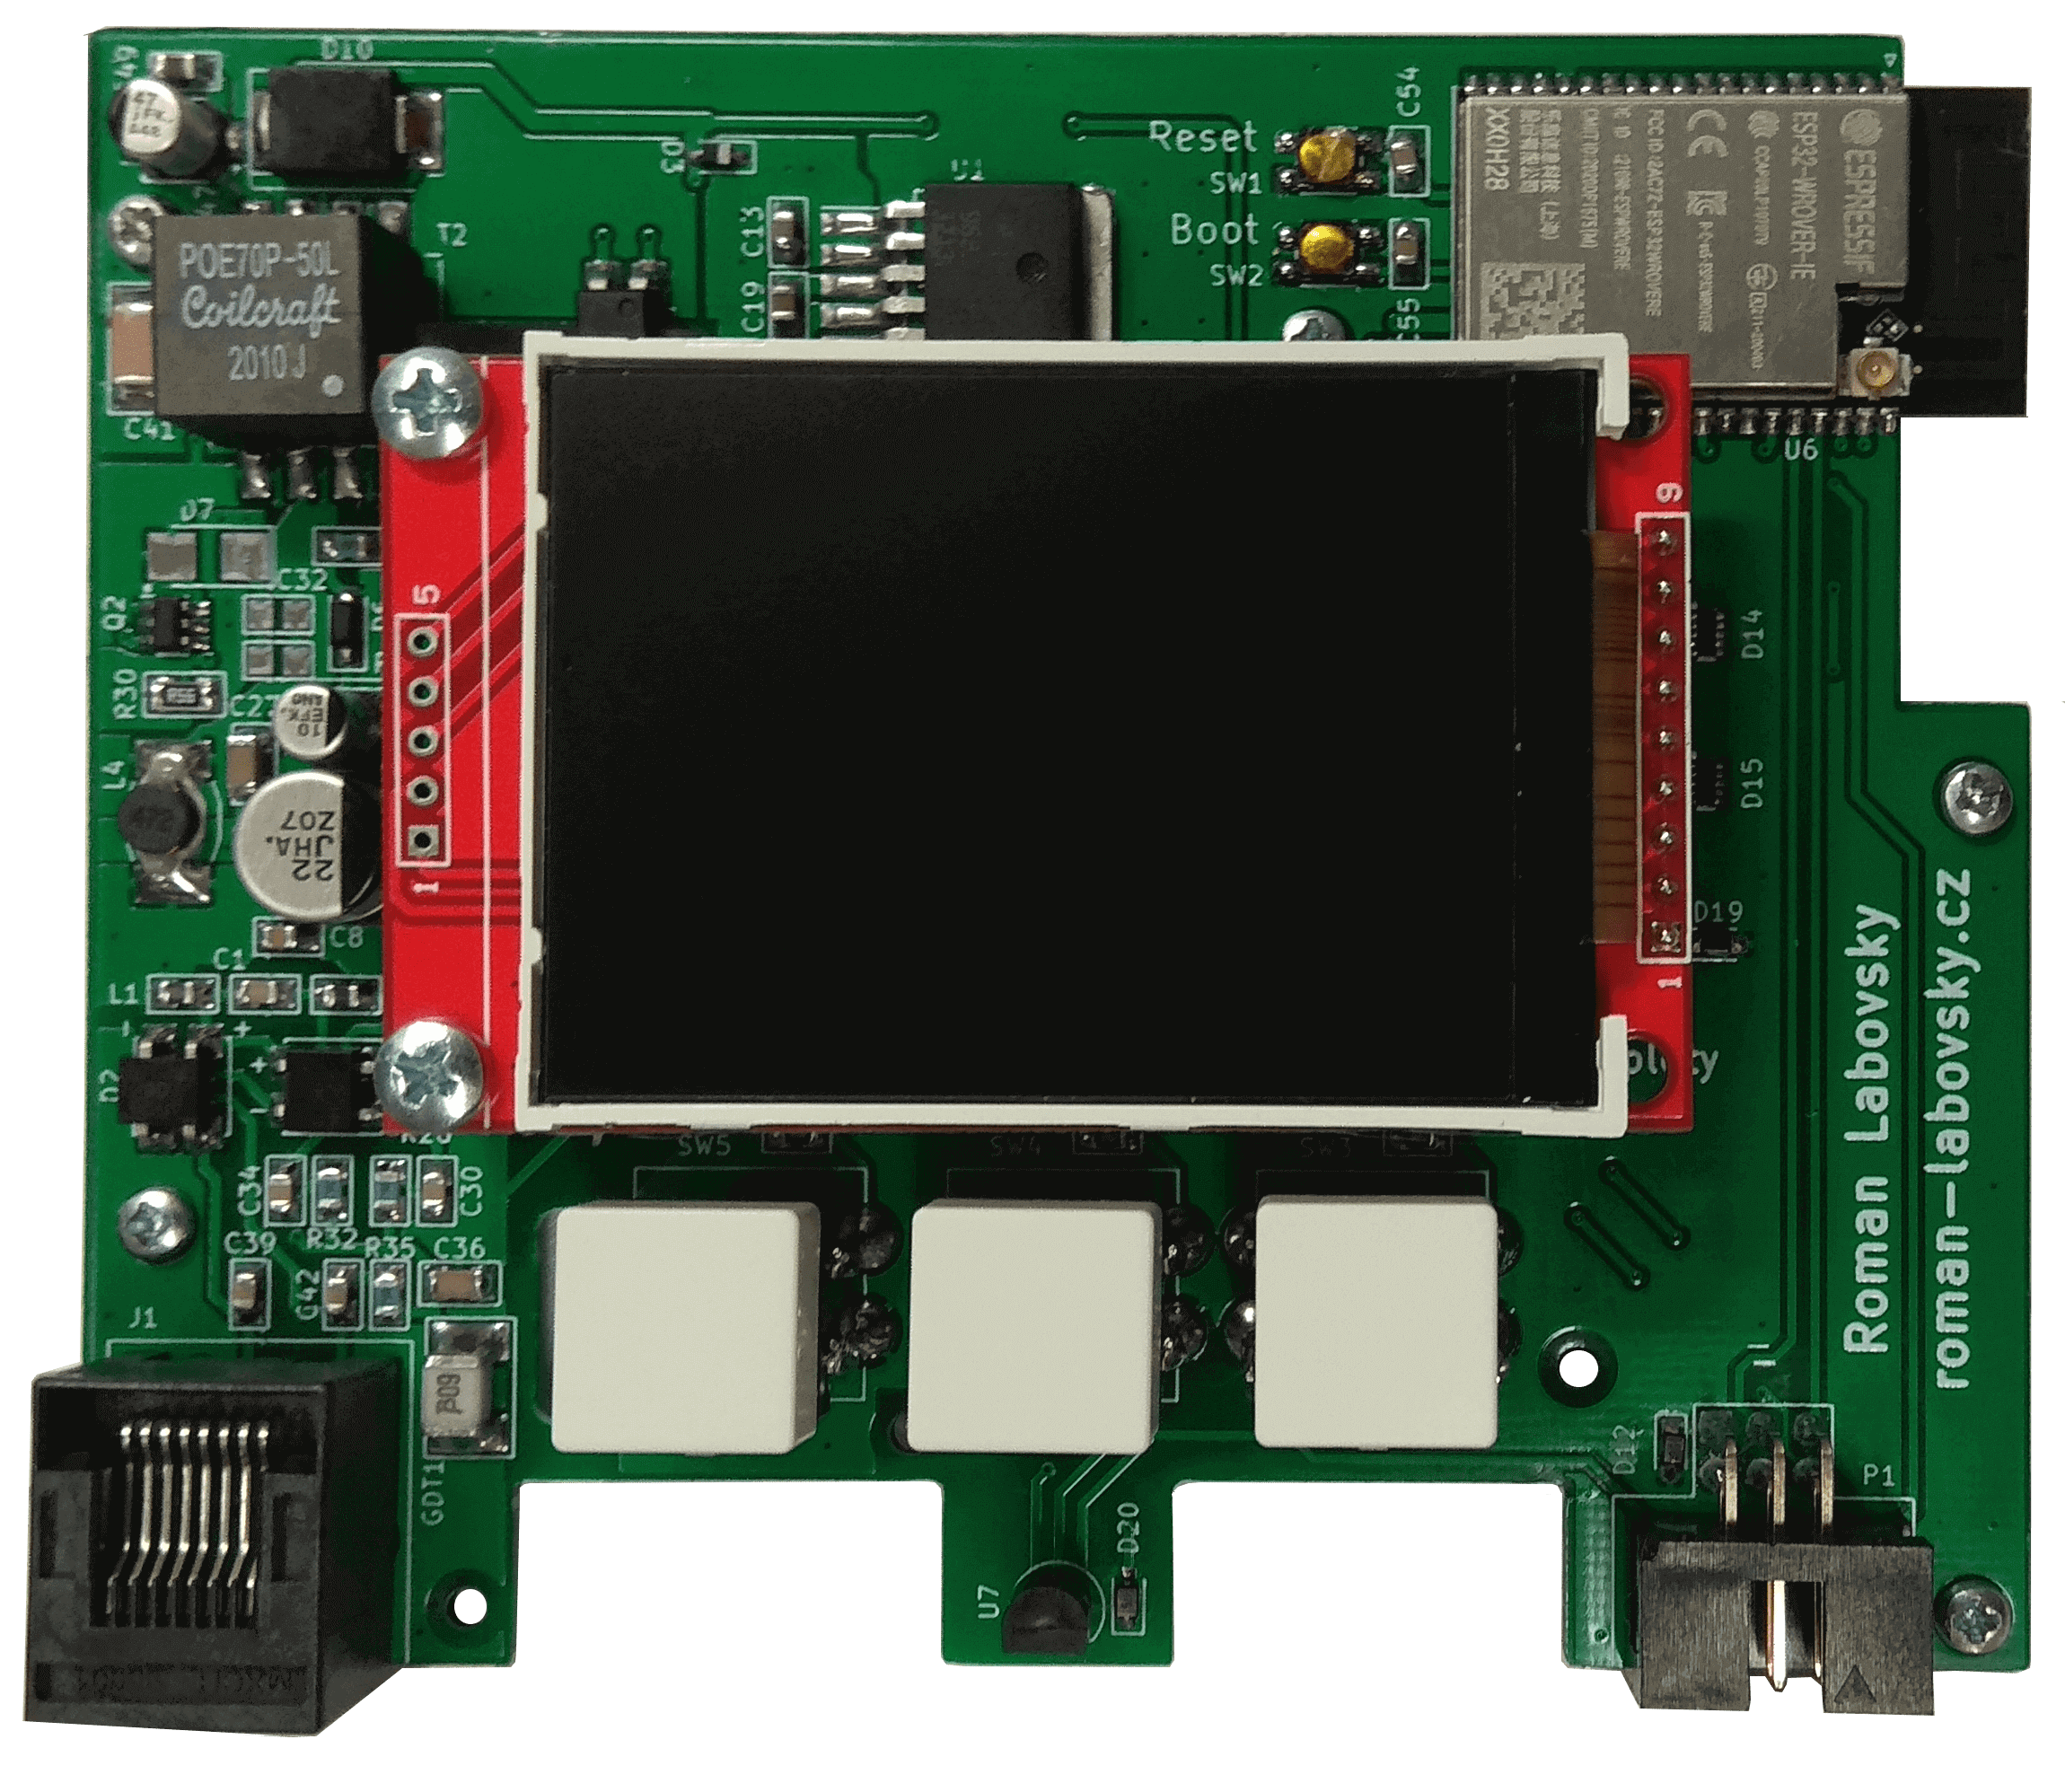
\includegraphics[width=0.88\textwidth]{images/nastenny-snimac-prostorove-teploty-ethernet/dps-nastenny-snimac-prostorove-teploty-ethernet-vrchni-cast-displej.png}
    \caption{DPS nástěnného snímače prostorové teploty s Ethernetem a~displejem, vrchní strana.}
    \label{fig:dps-nastenny-snimac-prostorove-teploty-ethernet-vrchni-cast-displej}
\end{figure}

\begin{figure}[H]
    \centering
    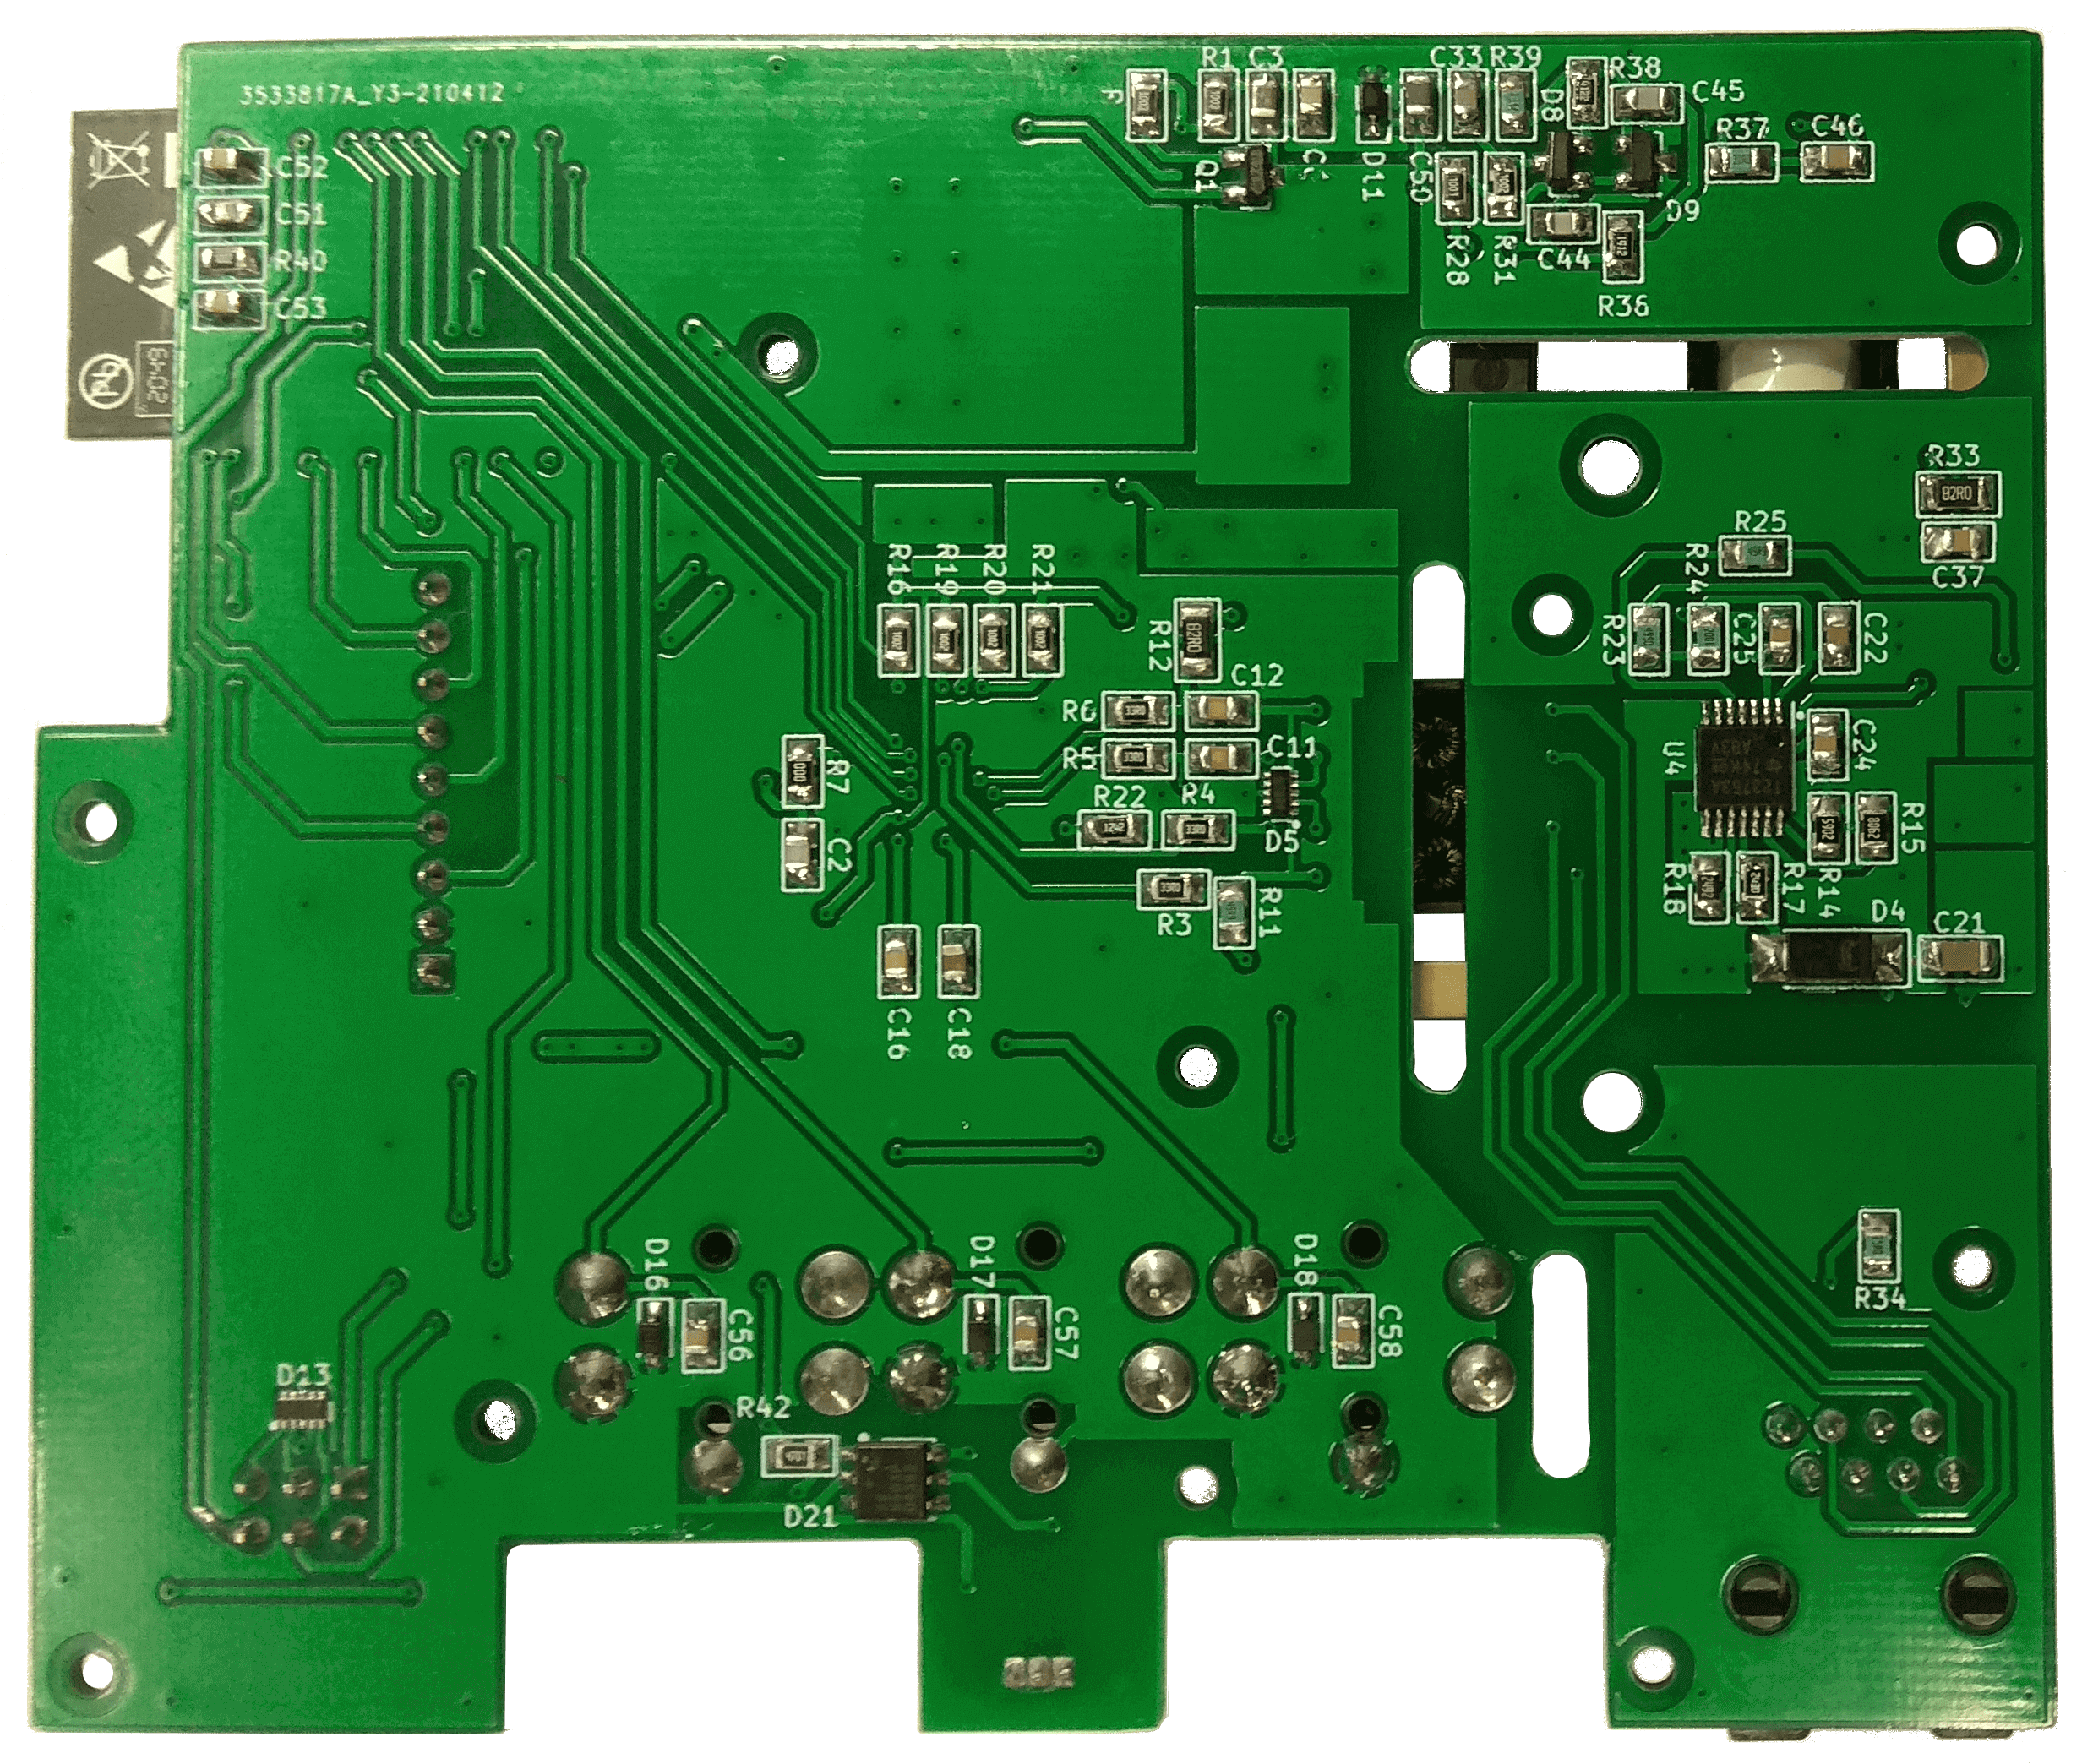
\includegraphics[width=0.88\textwidth]{images/nastenny-snimac-prostorove-teploty-ethernet/dps-nastenny-snimac-prostorove-teploty-ethernet-spodni-cast.png}
    \caption{DPS nástěnného snímače prostorové teploty s Ethernetem, spodní strana.}
    \label{fig:dps-nastenny-snimac-prostorove-teploty-ethernet-spodni-cast}
\end{figure}


\subsection{Varianta s WiFi}
\label{sec:wifi-modul}

Na obrázku \ref{fig:blokove-schema-nastenny-snimac-teploty-wifi} je blokové schéma nástěnného snímače prostorové teploty komunikující pomocí WiFi a je napájen pomocí síťového adaptéru. Oproti verzi z \ref{sec:ethernet-modul} chybí celá část tykající se POE napájení a také obvod W5500 implementující ethernetovou komunikaci. Zbylé části jsou totožné jako v části \ref{sec:ethernet-modul}.

V příloze \ref{app:nastenny-snimac-prostorove-teploty-wifi} je schéma snímací jednotky. Na obrázku \ref{fig:dps-nastenny-snimac-prostorove-teploty-wifi-vrchni-cast} je vrchní část realizované DPS pro snímací jednotku. Dále na obrázku \ref{fig:dps-nastenny-snimac-prostorove-teploty-wifi-vrchni-cast-displej} je DPS s osazeným displejem. Na obrázku \ref{fig:dps-nastenny-snimac-prostorove-teploty-wifi-spodni-cast} je spodní část DPS. Kompletní zařízení včetně umístění do krabičky a popis samotné krabičky je v části \ref{sec:krabicka-pro-nastenny-snimac-prostorove-teploty}.

\begin{figure}[H]
    \centering
    \def\svgwidth{\columnwidth}
    \input{images/svg/blokove-schema-nastenny-snimac-teploty-wifi.pdf_tex}
    \caption[]{Blokové schéma nástěnného snímače prostorové teploty s WiFi.}
    \label{fig:blokove-schema-nastenny-snimac-teploty-wifi}
\end{figure}

\begin{figure}[H]
    \centering
    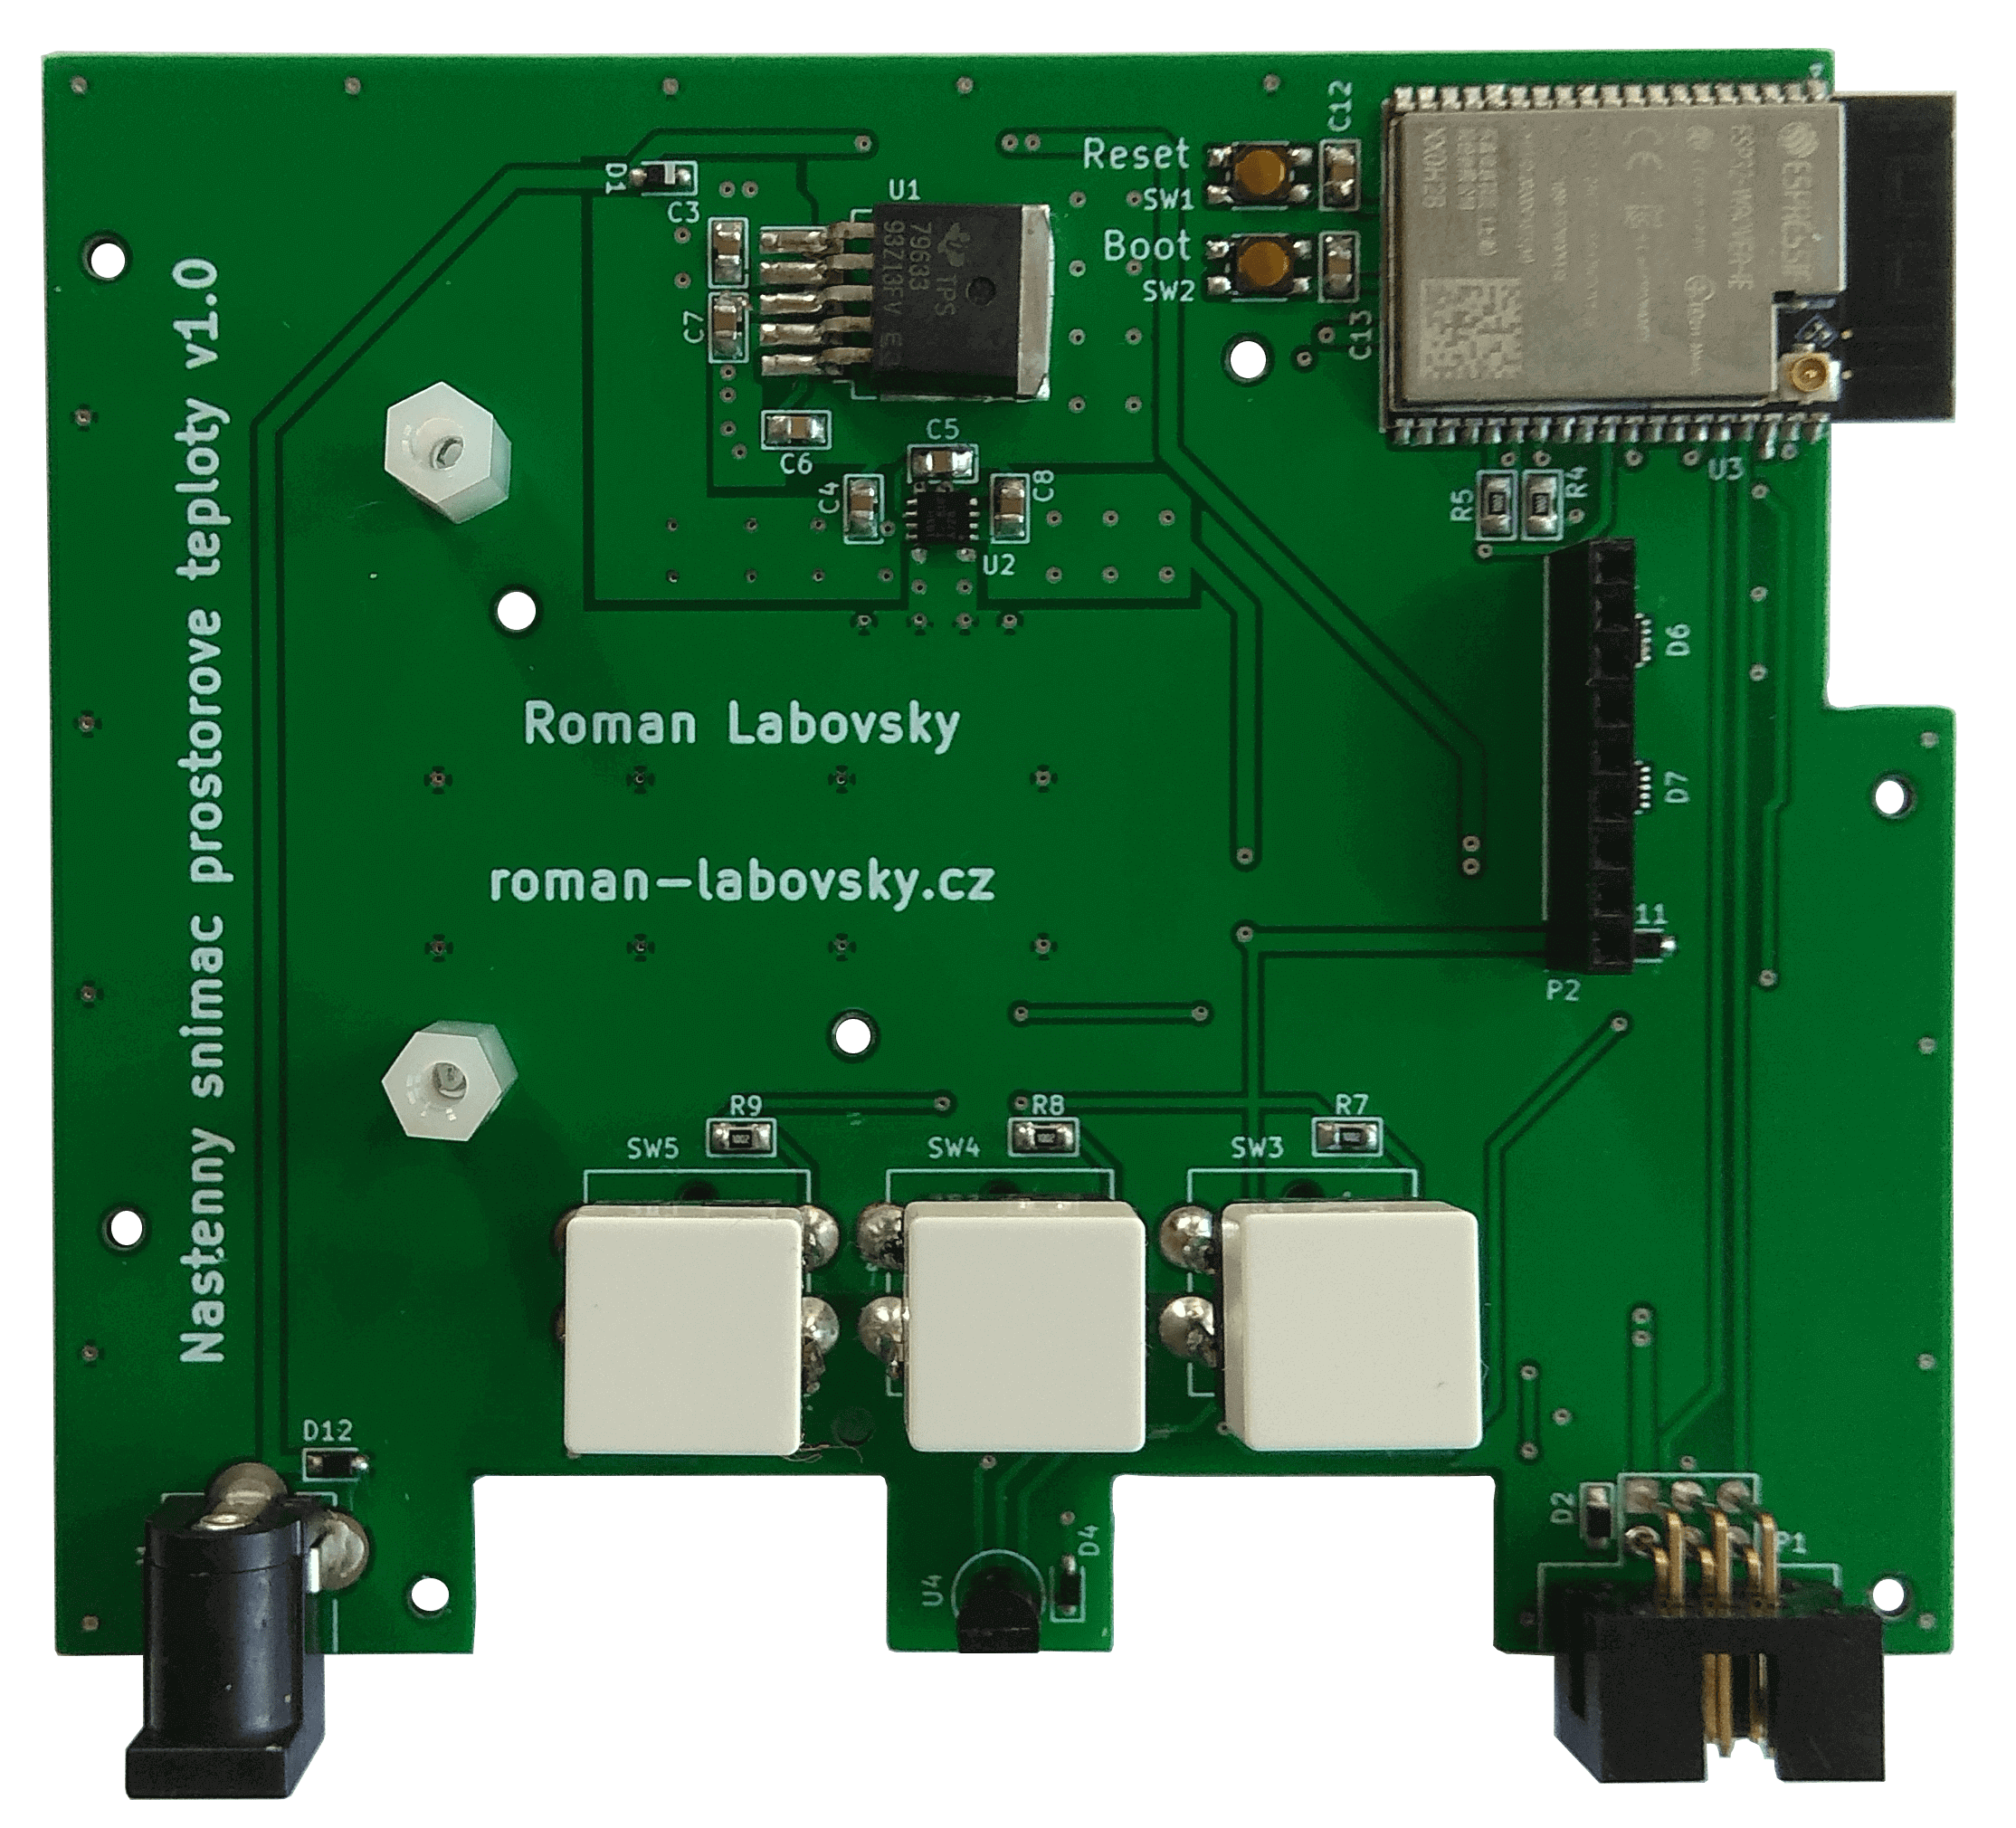
\includegraphics[width=0.85\textwidth]{images/nastenny-snimac-prostorove-teploty-wifi/dps-nastenny-snimac-prostorove-teploty-wifi-vrchni-cast.png}
    \caption{DPS nástěnného snímače prostorové teploty s WiFi, vrchní strana.}
    \label{fig:dps-nastenny-snimac-prostorove-teploty-wifi-vrchni-cast}
\end{figure}

\begin{figure}[H]
    \centering
    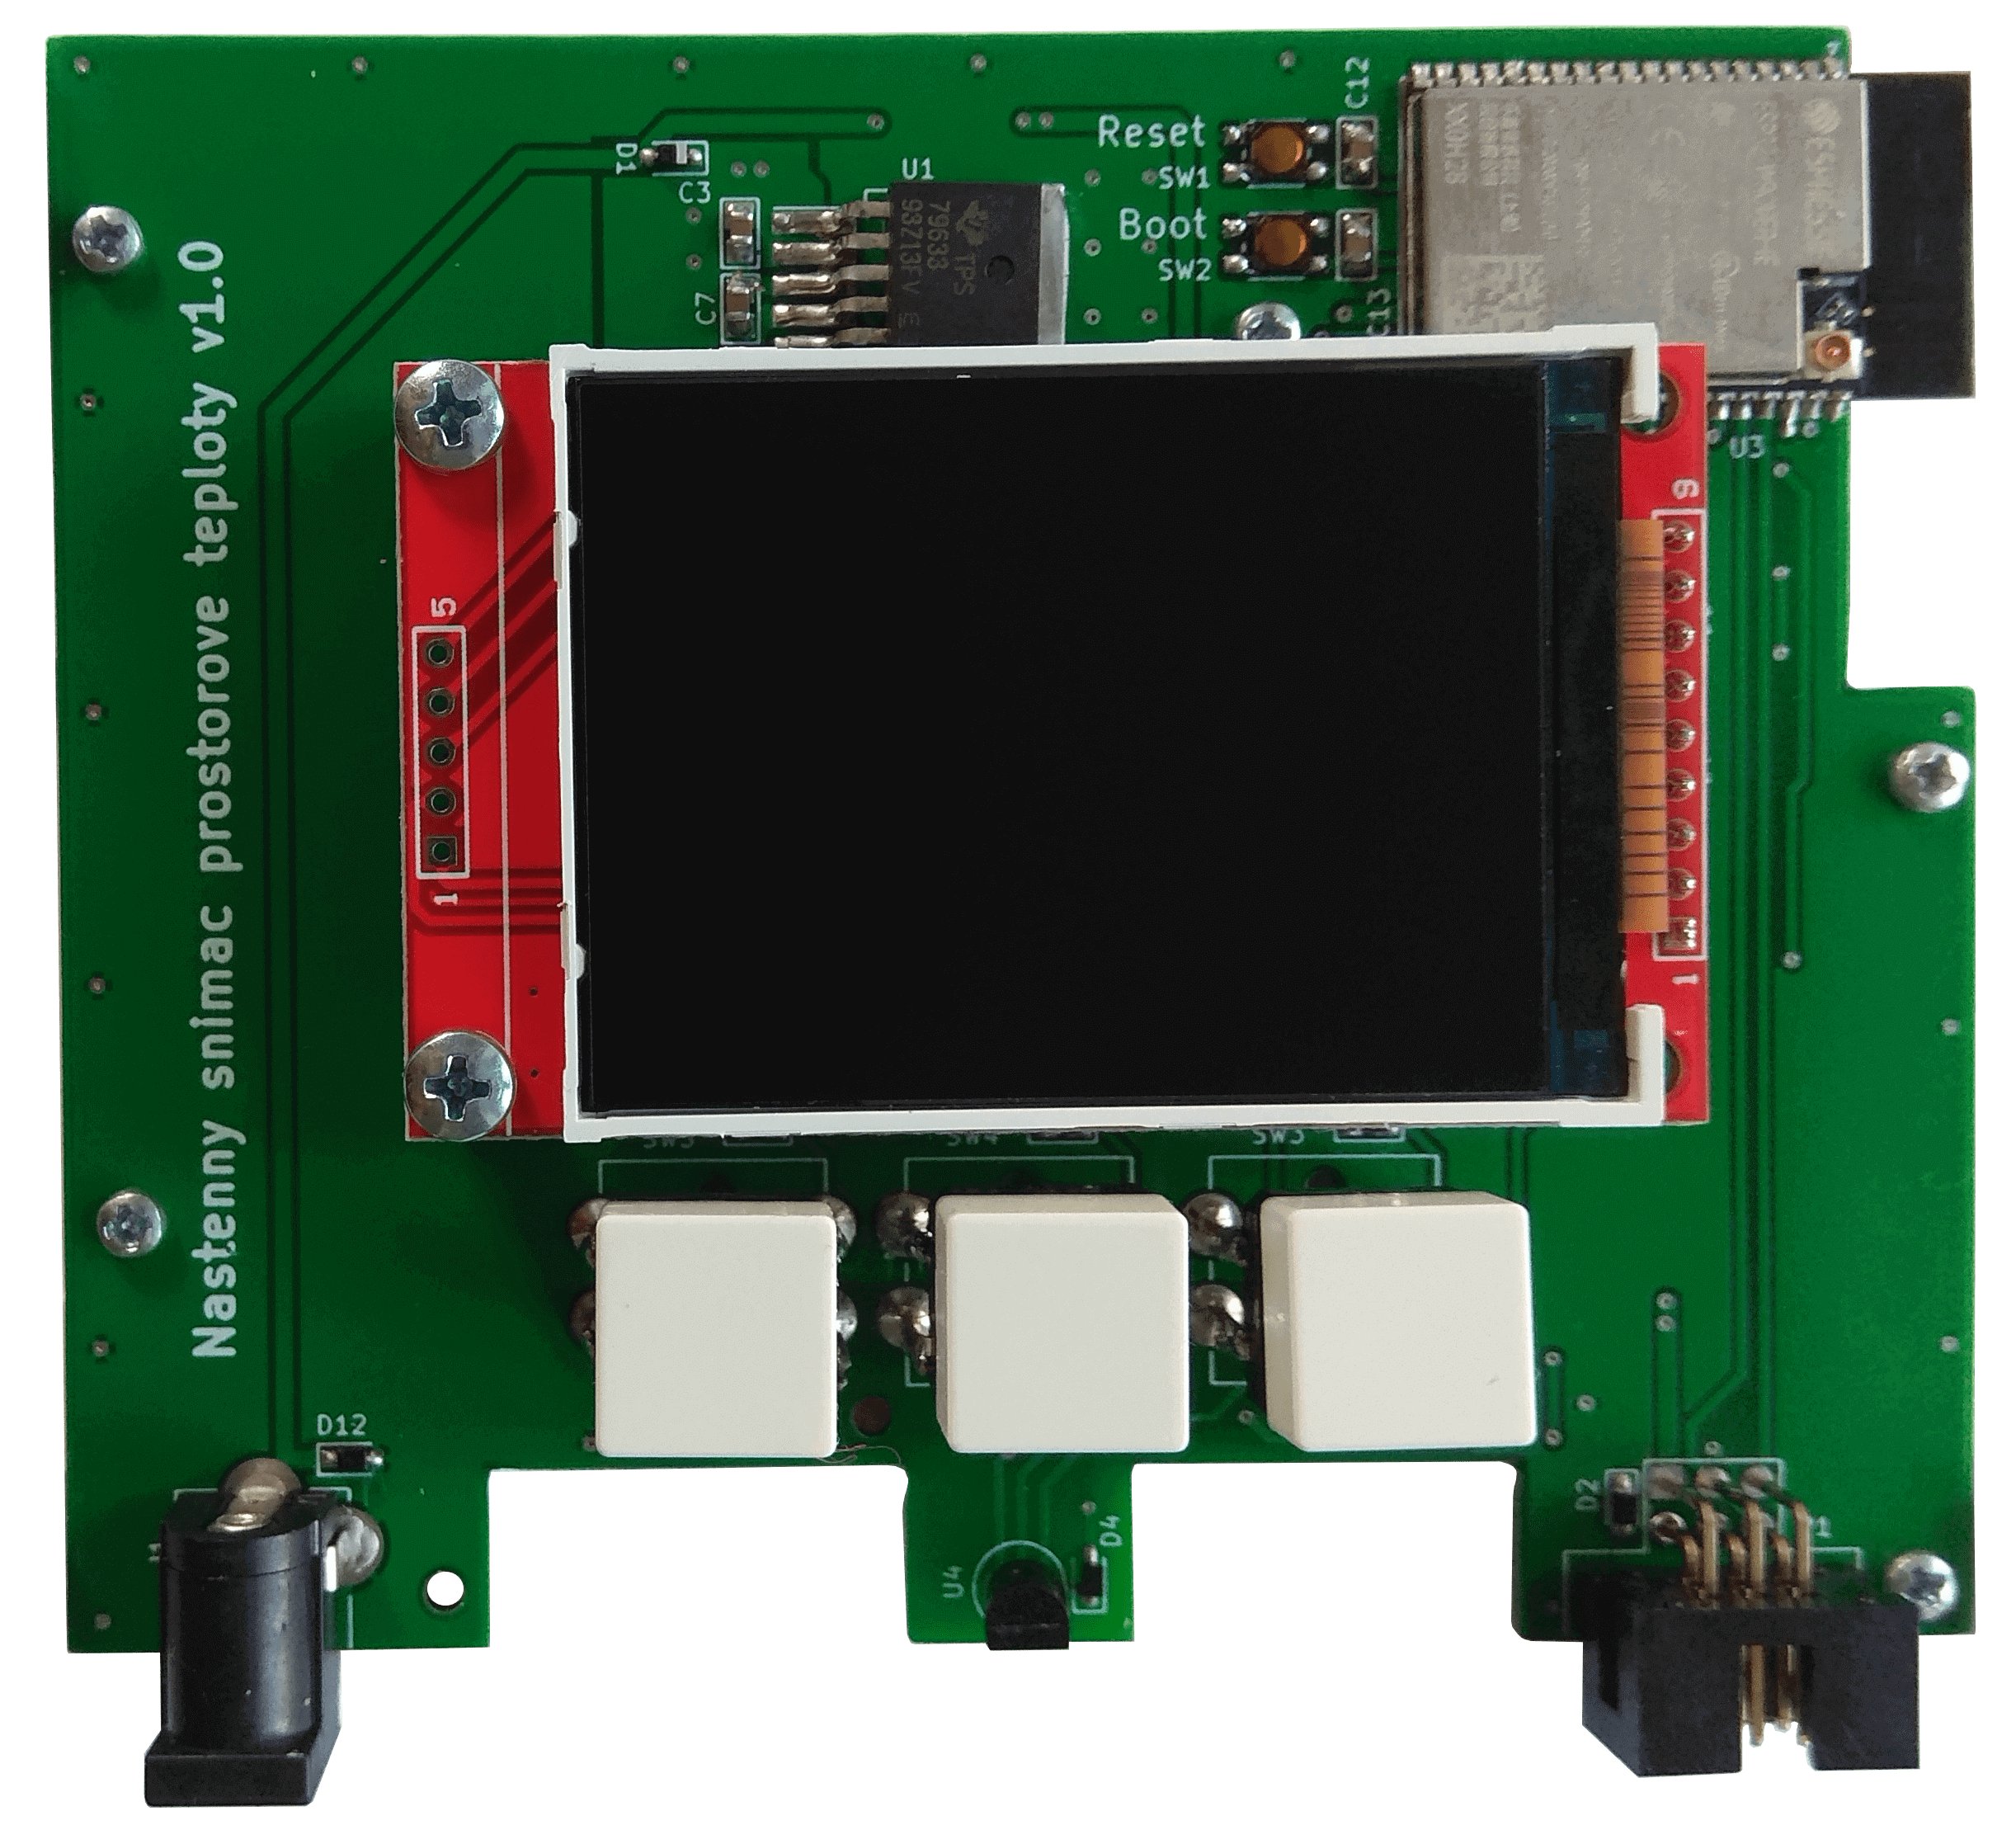
\includegraphics[width=0.85\textwidth]{images/nastenny-snimac-prostorove-teploty-wifi/dps-nastenny-snimac-prostorove-teploty-wifi-vrchni-cast-displej.png}
    \caption{DPS nástěnného snímače prostorové teploty s WiFi a displejem, vrchní strana.}
    \label{fig:dps-nastenny-snimac-prostorove-teploty-wifi-vrchni-cast-displej}
\end{figure}

\begin{figure}[H]
    \centering
    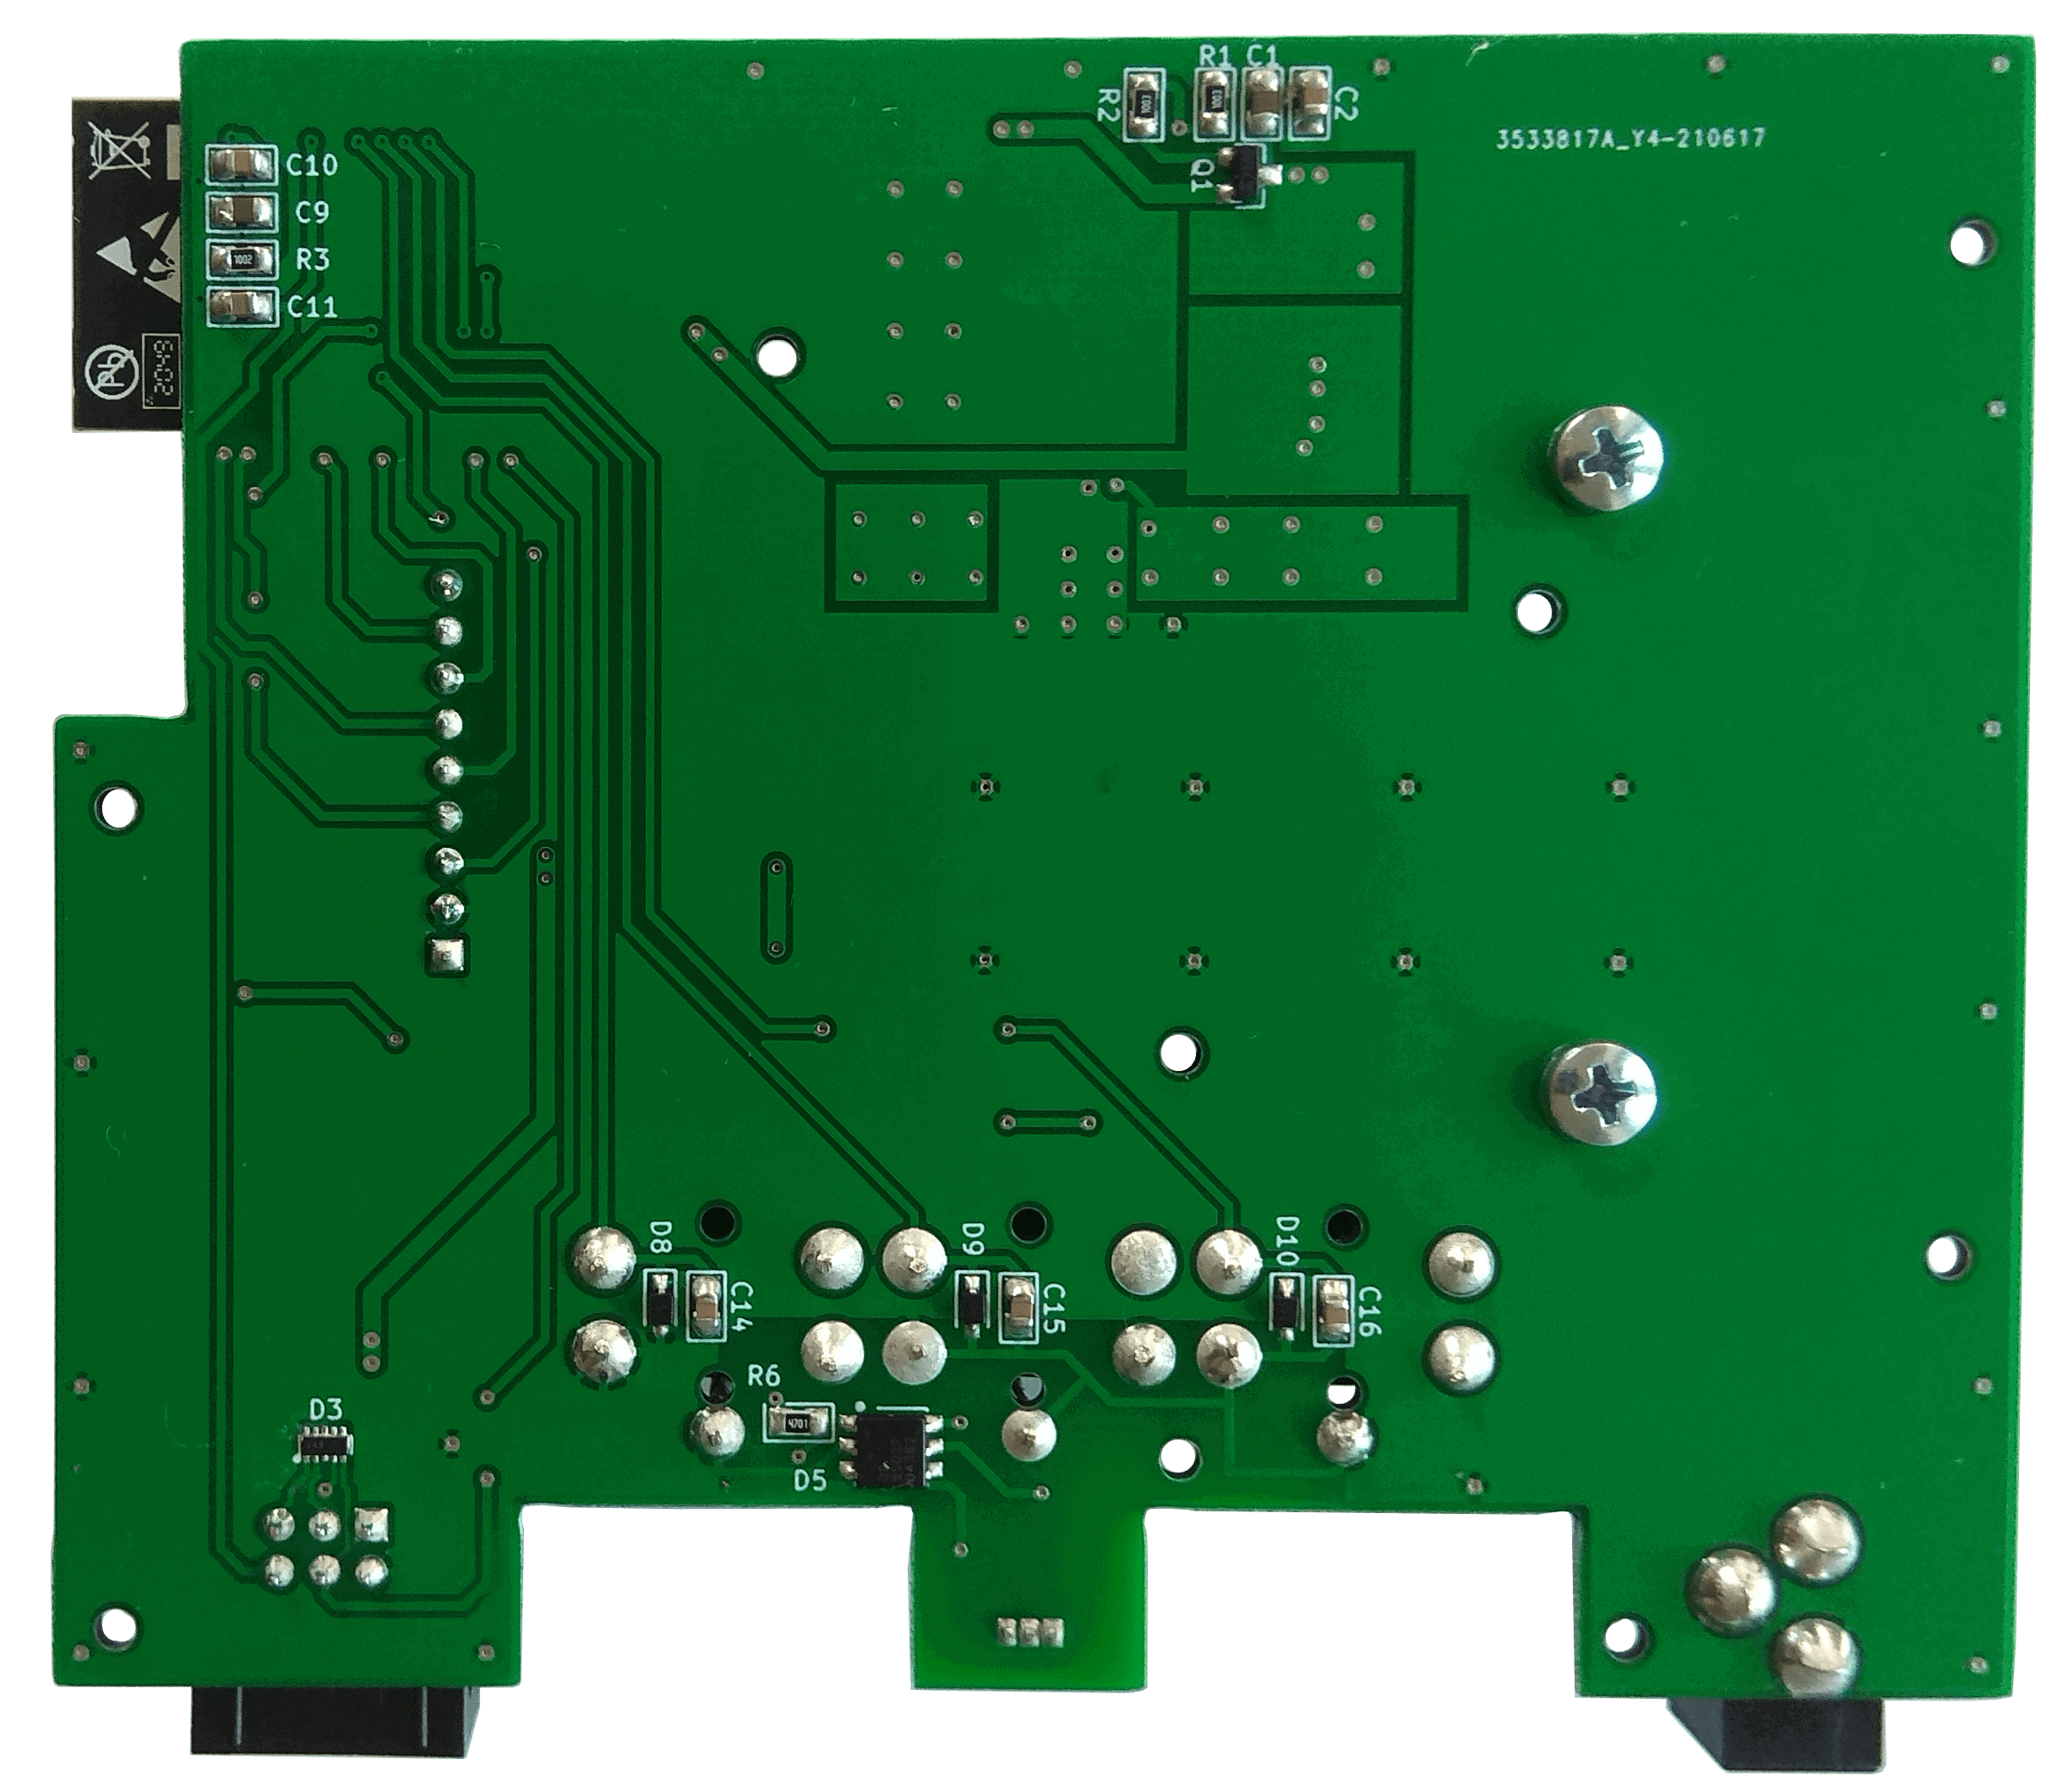
\includegraphics[width=0.89\textwidth]{images/nastenny-snimac-prostorove-teploty-wifi/dps-nastenny-snimac-prostorove-teploty-wifi-spodni-cast.png}
    \caption{DPS nástěnného snímače prostorové teploty s WiFi, spodní strana.}
    \label{fig:dps-nastenny-snimac-prostorove-teploty-wifi-spodni-cast}
\end{figure}

\section{Krabička pro nástěnný snímač prostorové teploty}
\label{sec:krabicka-pro-nastenny-snimac-prostorove-teploty}
Krabička pro \acrshort{nspt} je vytisknuta na 3D tiskárně Prusa i3 MK3s \cite{prusa-i3-mk3s+} (čelní strana je na obrázku \ref{fig:krabicka-nastenny-snimac-prostorove-teploty-predni-strana-displej}). Použitý plast je \acrshort{pet-g} \cite{prusament} (\textit{\acrlong{pet-g}}), bílá barva byla požadovaná uživatelem. Výhody zejména tohoto materiálu jsou houževnatost, pevnost a dobré propojování vrstev při tisku. Návrh modelu byl realizován v~softwaru FreeCAD \cite{freecad}. Samotná příprava modelu pro tisk je v~PrusaSliceru \cite{prusaslicer}. Krabička má rozměry 130~×~99~×~26~mm a skládá ze dvou dílů. Krabička jak pro verzi s Ethernetem, tak i pro WiFi je stejná, liší se jen konektorem pro RJ45 a DC konektorem pro adaptér.

Spodní díl slouží k uchycení DPS, která je umístěná na distančních sloupkách (dochází tak k~lépe odvádění tepla ze součástek). Spodní díl má v horní části průduchy na odvětrávání tepla. Ve spodní části je vymezená oblast s~průduchy pro teplotní senzor, který se nachází nad nimi. Dále je tato oblast ohraničená přepážkou, aby nedocházelo přílišnému míchání vzduchu z prostoru DPS a~teplotního senzoru. Na obvodu se nacházejí sloupky pro uchycení horní části krabičky. Distanční sloupky i sloupky pro horní části obsahují v~otvoru závitovou vložku, dochází tak optimální přidělání dílů za pomocí metrického šroubku (nedochází k pnutí a možnému prasknutí jako v~případě, pokud by se použil samovrtný šroubek). Dále se na spodním dílu nacházejí čtyři díry pro uchycení na zeď, v jejich oblasti je plast ještě zesílen. Na druhé straně spodního dílu jsou distanční sloupky, které slouží k~tomu, aby při přivrtání ke zdi, krabička neležela přímo na zdi, aby docházelo k odvětrávání horní části krabičky a k proudění vzduchu ve spodní části v oblasti teplotního senzoru.

Horní část krabičky obsahuje otvory pro displej a tlačítka. Na čelní straně se nacházejí uprostřed průduchy pro teplotní senzor, dále uvnitř této oblasti je vytvořená přepážka, která dosedá na spodní část přepážky spodního dílů, tato vzduchová kapsa je tedy oddělená od zbytku krabičky, aby teplotní senzor nebyl ovlivněn moc teplotou samotné krabičky. Dále se na čelní straně nacházejí průchody pro konektor RJ45 pro variantu s Ethernetem nebo průchod pro DC napájecí konektor, dále průchod pro programovací konektor. Horní část je přichycena ke spodní čtyřmi šroubky, jejichž hlavičky jsou utopené a~nepřečnívají na povrchu.

Jednotlivé díly jsou zobrazeny v příloze \ref{app:krabicka-pro-nastenny-snimac-prostorove-teploty}, dále jsou zde fotografie části krabičky s umístěnou DPS. Krabička je poměrně robustní, spodní tlouštka stěny je 2 mm, obvodové stěny jsou též 3 mm silné a čelní strana má 2 mm. Samotné uchycení na stěnu je velmi stabilní. U verze s Ethernetem je chyba v návrhu v DPS, spočívající nedostatečném vysunutí konektorů z DPS, což je vidět, že konektory nejsou zarovnané s čelní stranou krabičky, nicméně na funkčnost používaní konektorů to nemá vliv. Ve verzi s WiFi je tato chyba opravena. Hmatníky na tlačítka byly zakoupeny.
 
\begin{figure}[H]
    \centering
    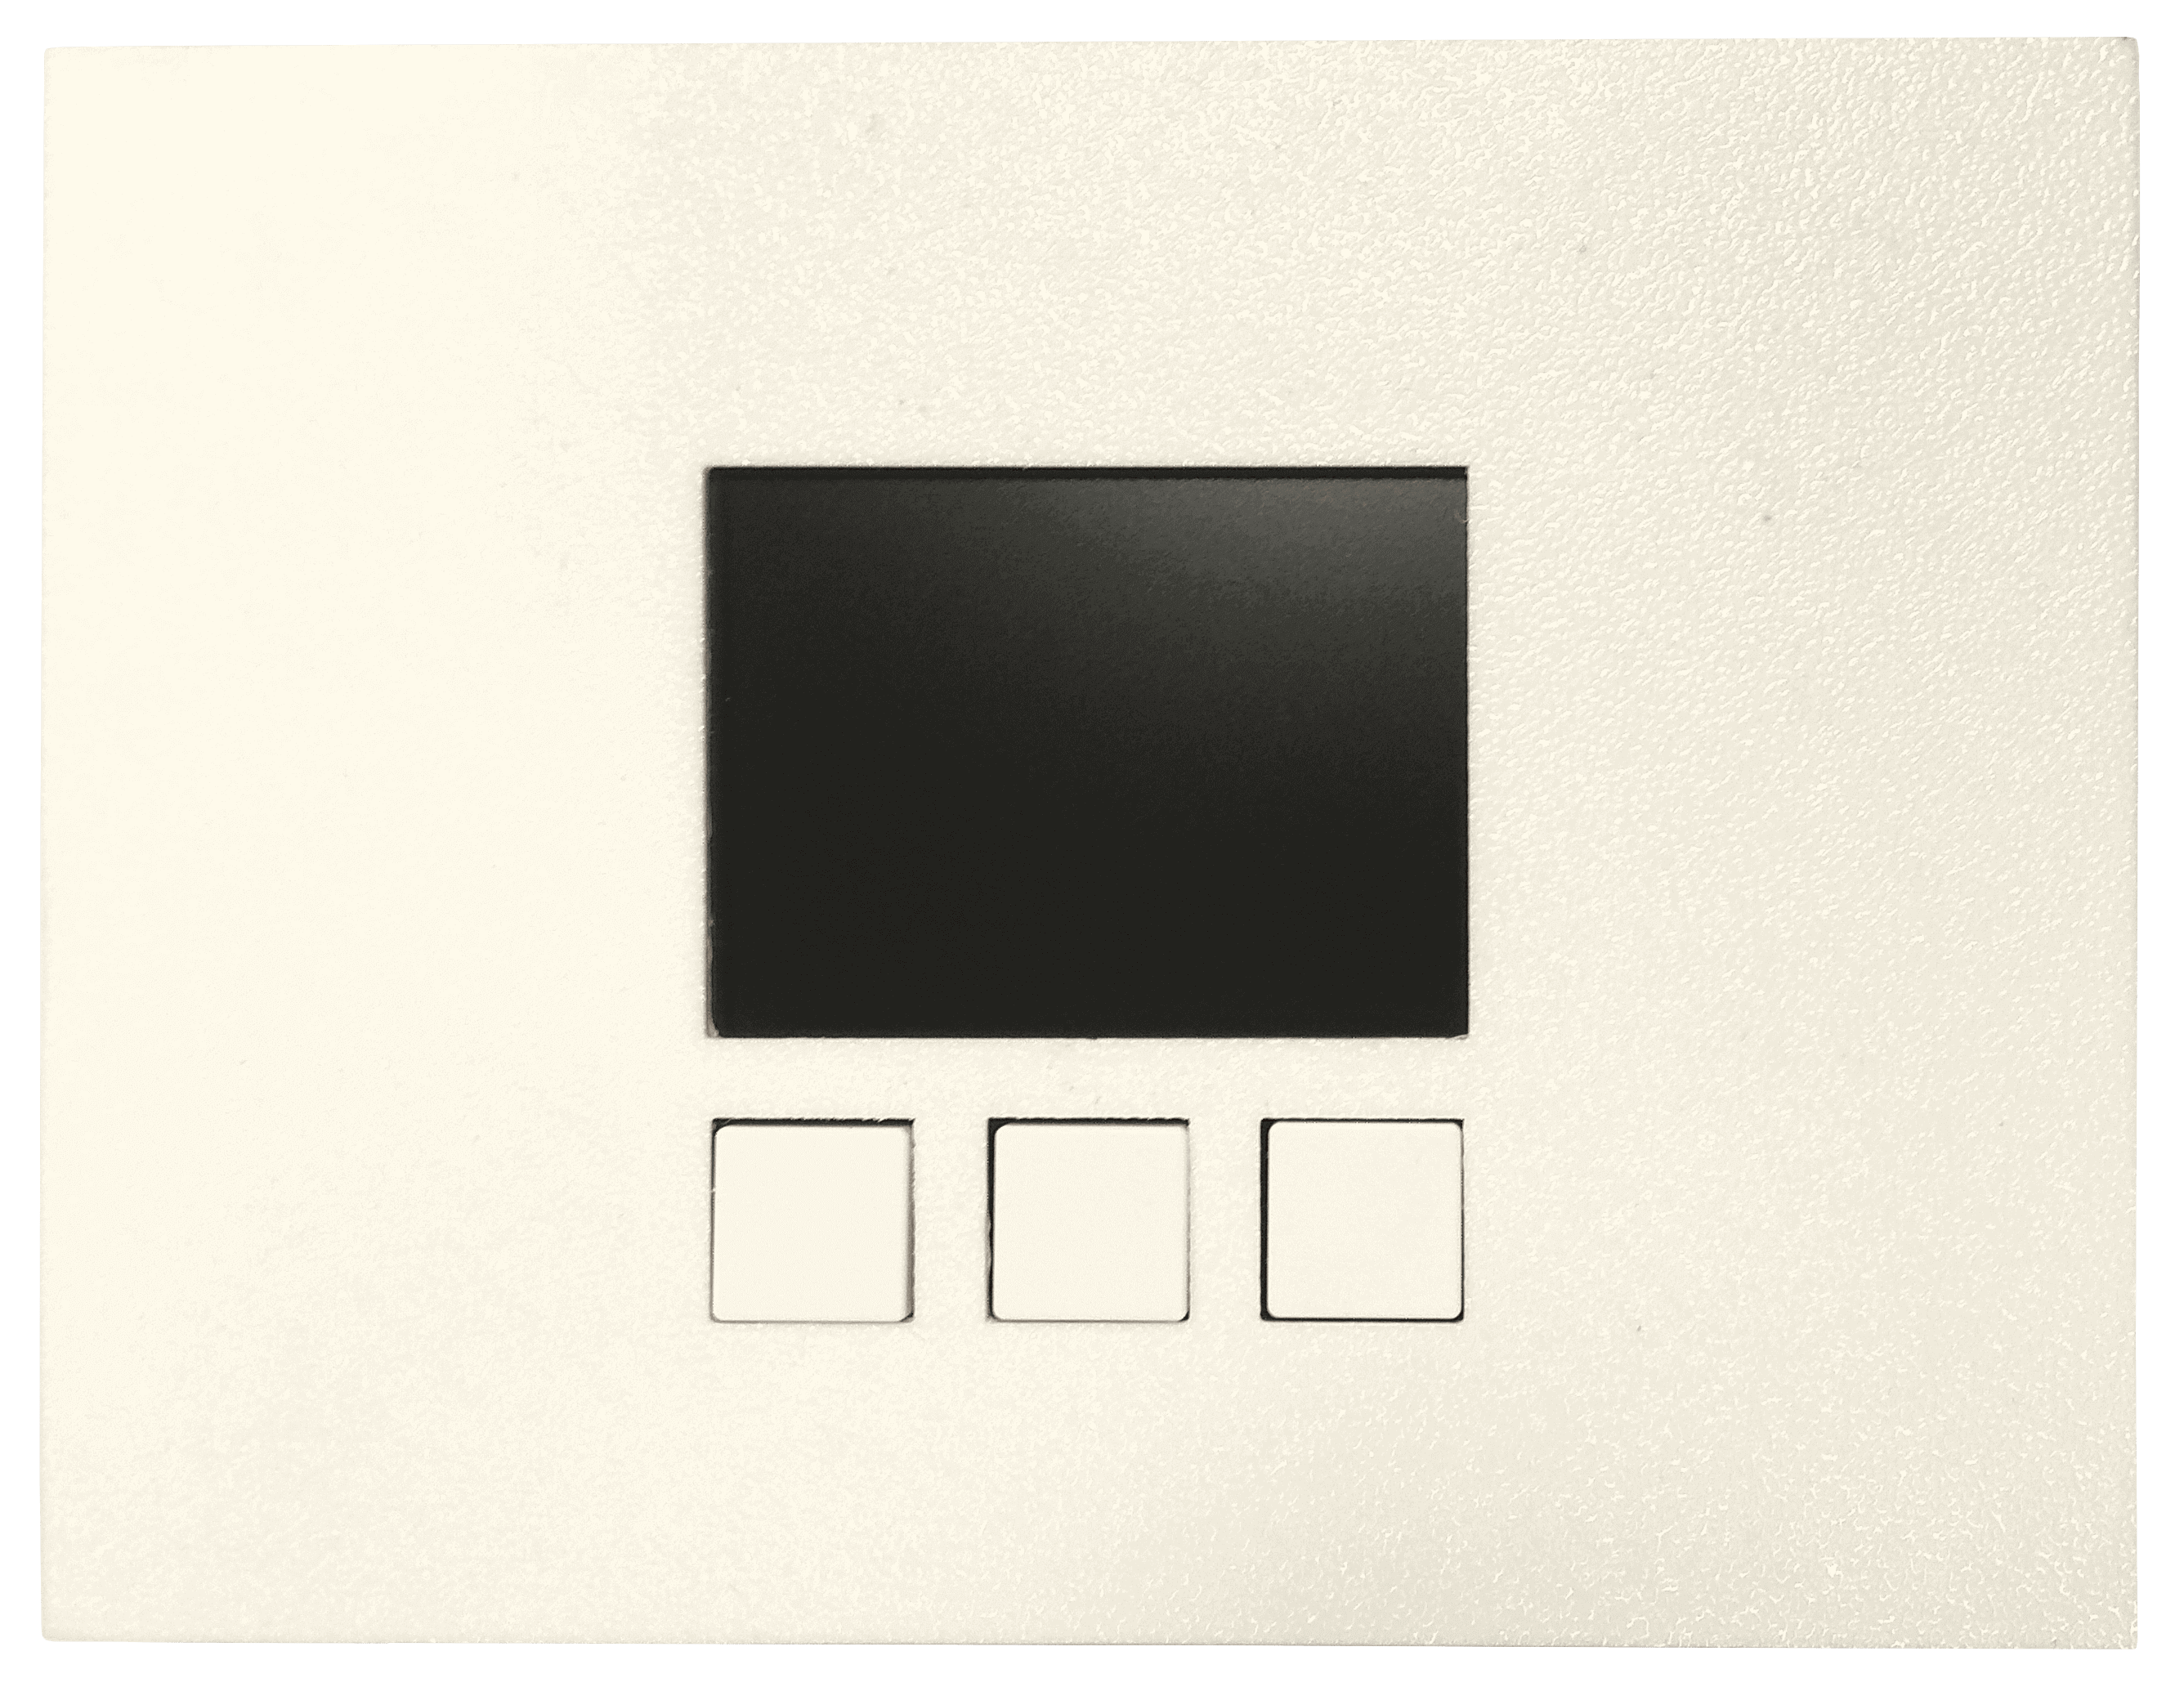
\includegraphics[width=0.89\textwidth]{images/krabicka-nastenny-snimac-prostorove-teploty/krabicka-nastenny-snimac-prostorove-teploty-predni-strana-displej.png}
   \caption{Čelní strana krabičky.}
    \label{fig:krabicka-nastenny-snimac-prostorove-teploty-predni-strana-displej}
\end{figure}

\section{Převodník USB-UART CP2102N}
\label{sec:prevodnik-usb-uart-cp2102n}
Pro programování \acrshort{nspt}, přesněji modulu ESP32 Wrover-IE je použit převodní USB-UART CP2102N \cite{cp2102n-miniek} od firmy Silocon Labs. Byl zvolen modul CP2102N MINEK (obrázek \ref{fig:prevodnik-cp2102n-modul-vrchni-cast}). Modul je doplněn o zapojení tranzistoru pro automatický reset a~automatický boot modulu (obrázek \ref{fig:prevodnik-cp2102n-modul-spodni-cast}). Z modulu se využívají signály \acrshort{dtr} (\textit{\acrlong{dtr}}) a \acrshort{rts} (\textit{\acrlong{rts}}). Pokud je potřeba vstoupit do bootloaderu pro nahrání nového firmwaru, je nutné podržet boot a~následně stisknout reset, zařízení je tak připraveno nahrát nový firmware. V případě využití signálu DTR a RTS se tato operace dělá automaticky, nicméně z~pravdivostní tabulky \ref{tab:pravdivostni-tabulka-pro-automaticky-boot} není vidět stav pro EN = 0, IO0 = 0, tento stav je zajištěn pomocí kondenzátoru o velikosti 1\textmu  F mezi EN vstup a~GND. Tímto kondenzátorem se zajistí zpoždění při přechodu z log. 0 na log. 1 na vstupu EN, zároveň v~tomto zpoždění je vstup IO0 v log. 0 a je možné vstoupit do bootloaderu. Z modulu jsou do konektoru vyvedeny 5 V, GND, RXD, TXD, EN a IO0. Komunikace mezi CP2102N a modulem ESP32 pak probíhá po vodičích RXD a TXD. Schéma zapojení pro automatický bootloader s~využitím modulu CP2102N MINEK je v příloze \ref{app:schemata-ostatni}.

\begin{center}
\begin{table}[H]
\begin{tabular}{ |c|c||c|c| }  
 \hline
 \thead{DTR} & \thead{RTS} & \thead{EN} & \thead{IO0}\\
 \hline
 1 & 1 & 1 & 1 \\ 
 0 & 0 & 1 & 1 \\ 
 1 & 0 & 0 & 1 \\ 
 0 & 1 & 1 & 0 \\ 
 \hline
\end{tabular}
 \caption{Pravdivostní tabulka pro automatický boot modulu ESP32.}
 \label{tab:pravdivostni-tabulka-pro-automaticky-boot}
\end{table}
\end{center}


%\begin{figure}[H]
%    \centering
%    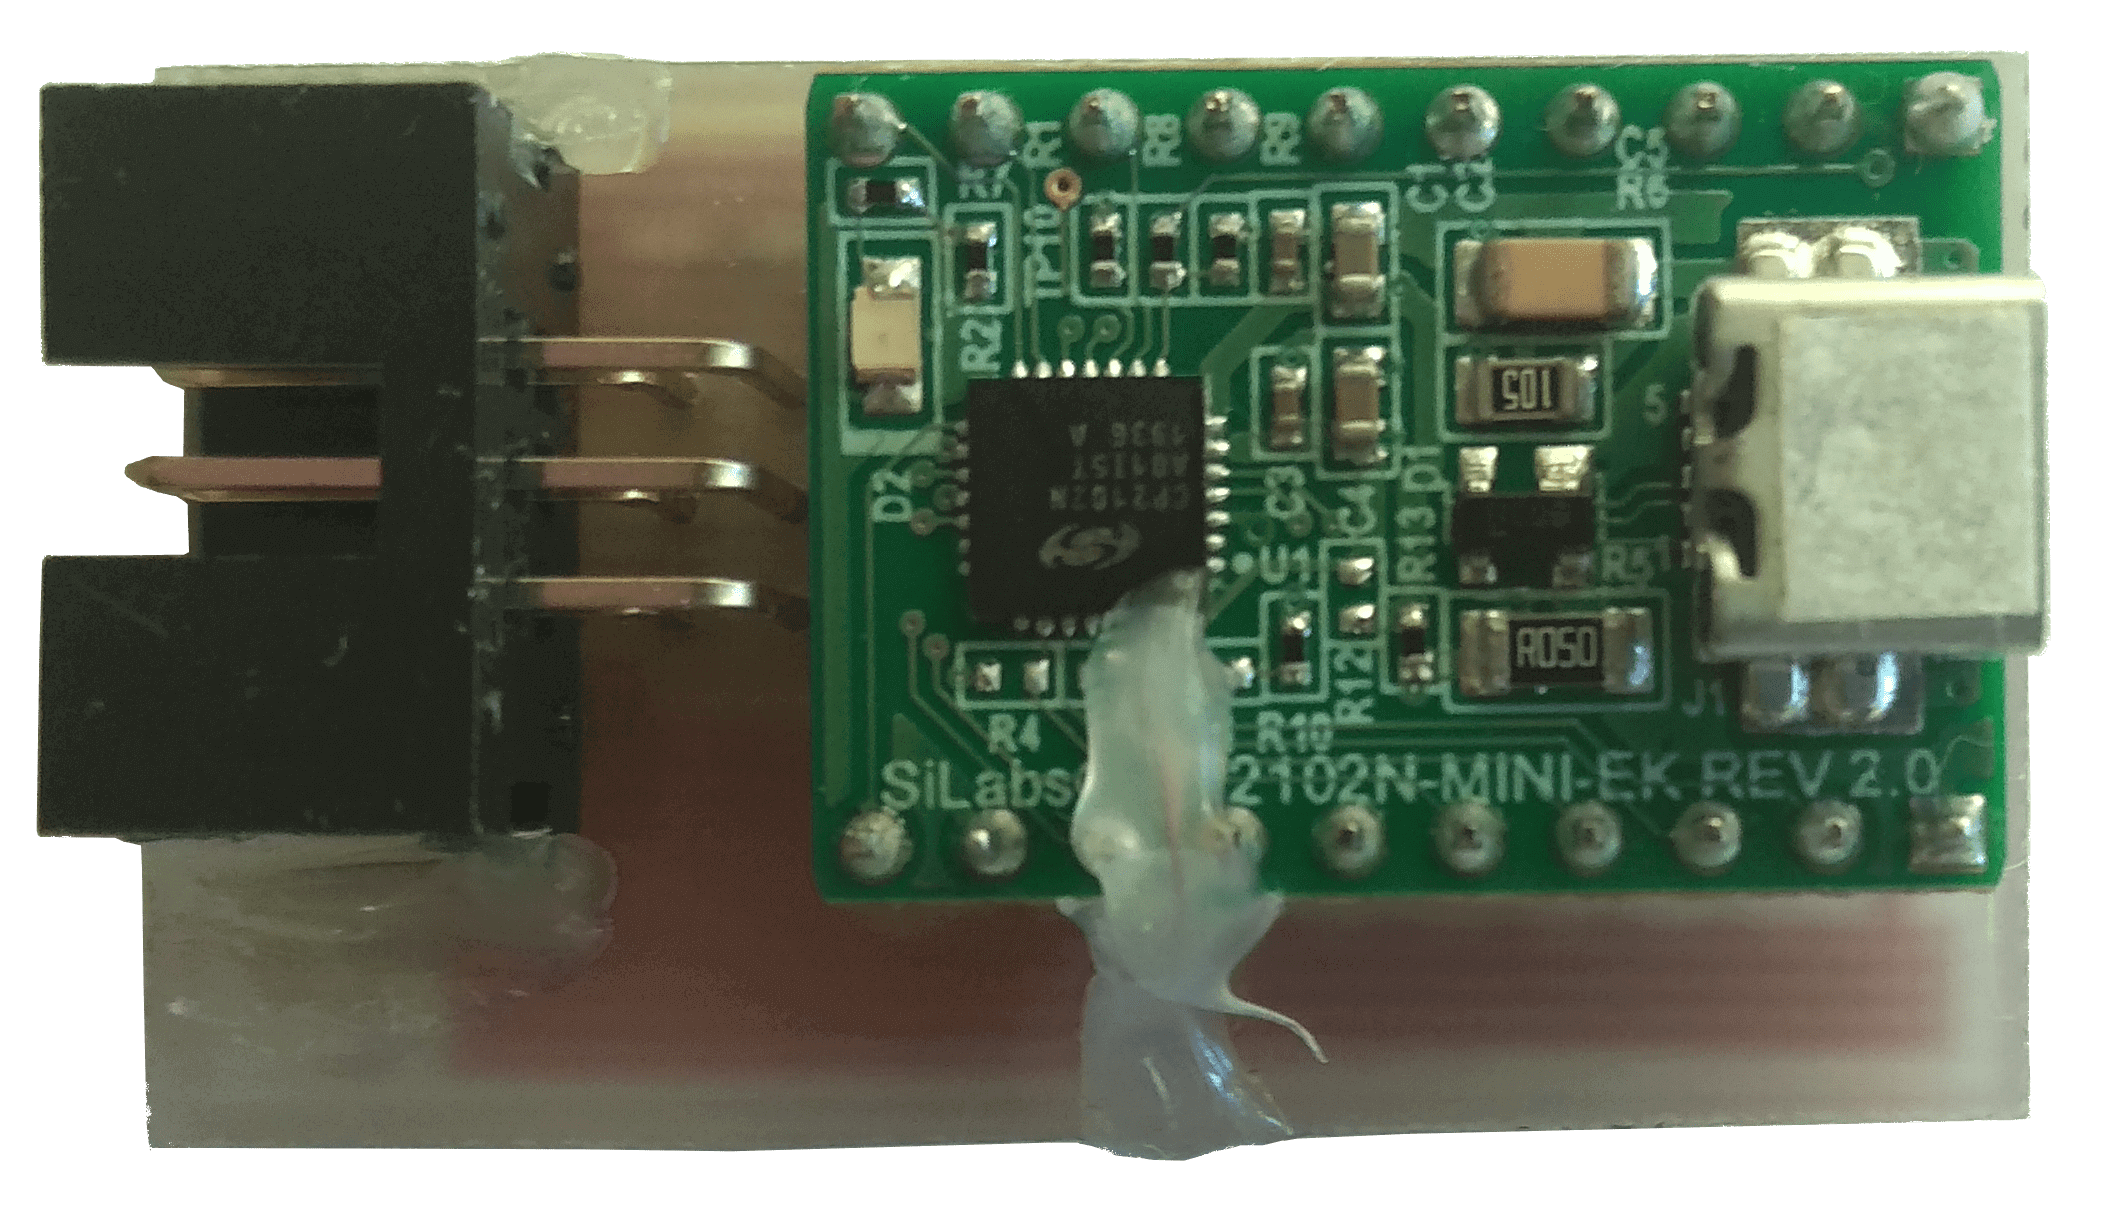
\includegraphics[width=0.5\textwidth]{images/prevodnik-usb-uart-cp2102n/prevodnik-cp2102n-modul-vrchni-cast.png}
%    \caption[Vrchní část modulu převodníku USB-UART.]{Vrchní část modulu převodníku USB-UART CP2102N MINEK s~výstupním konektorem pro programování zařízení.}
%    \label{fig:prevodnik-cp2102n-modul-vrchni-cast}
%\end{figure}


%\begin{figure}[H]
%    \centering
%    \includegraphics[width=0.5\textwidth]{images/prevodnik-usb-uart-cp2102n/prevodnik-cp2102n-modul-spodni-cast.png}
%    \caption[Spodní část modulu převodníku USB-UART.]{Spodní část modulu převodníku USB-UART s doplněnými tranzistory pro signály DTR a RTS pro automatický bootloader.}
%    \label{fig:prevodnik-cp2102n-modul-spodni-cast}
%\end{figure}



\begin{figure}[H]
\centering
\begin{subfigure}{.5\textwidth}
    \centering
    \includegraphics[width=\textwidth]{images/prevodnik-usb-uart-cp2102n/prevodnik-cp2102n-modul-vrchni-cast.png}
    \caption[Vrchní část modulu převodníku USB-UART.]{Vrchní část modulu převodníku USB-UART CP2102N MINEK s~výstupním konektorem pro programování zařízení.}
    \label{fig:prevodnik-cp2102n-modul-vrchni-cast}
\end{subfigure}%
\begin{subfigure}{.5\textwidth}
    \centering
    \includegraphics[width=\textwidth]{images/prevodnik-usb-uart-cp2102n/prevodnik-cp2102n-modul-spodni-cast.png}
    \caption[Spodní část modulu převodníku USB-UART.]{Spodní část modulu převodníku USB-UART s~doplněnými tranzistory pro signály DTR a RTS pro automatický bootloader.}
    \label{fig:prevodnik-cp2102n-modul-spodni-cast}
\end{subfigure}
\caption{Převodníku USB-UART CP2102N MINEK.}
\label{fig:prevodnik-cp2102n}
\end{figure}


